\section{Estudio de Calidad de Imagen}

En esta sección se estudiaron configuraciones que afectan la calidad de imagen resultante. Para el estudio de diferencia entre imágenes se utilizó el software PerceptualDiff basado en el trabajo de Hector Yee y otros en 2001 \cite{Yee:2001:SSV:383745.383748}, este programa utiliza un modelo computacional imitando al ojo humano para generar la diferencia perceptual entre dos imágenes.

\subsection{Composición Final de Imagen}
\label{subsec:final}
Todas las imágenes en esta sección fueron renderizadas con una resolución de pantalla de $1920x1080$, con una resolución para la representación de vóxeles de $512^3$ y con una longitud de marcha del cono de $0.5$. La representación de vóxeles solo contiene iluminación directa.

\begin{figure}[H]
	\centering
	\begin{subfigure}[t]{.49\linewidth}
		\centering
		\captionsetup{justification=centering}
		\caption*{Directa}
		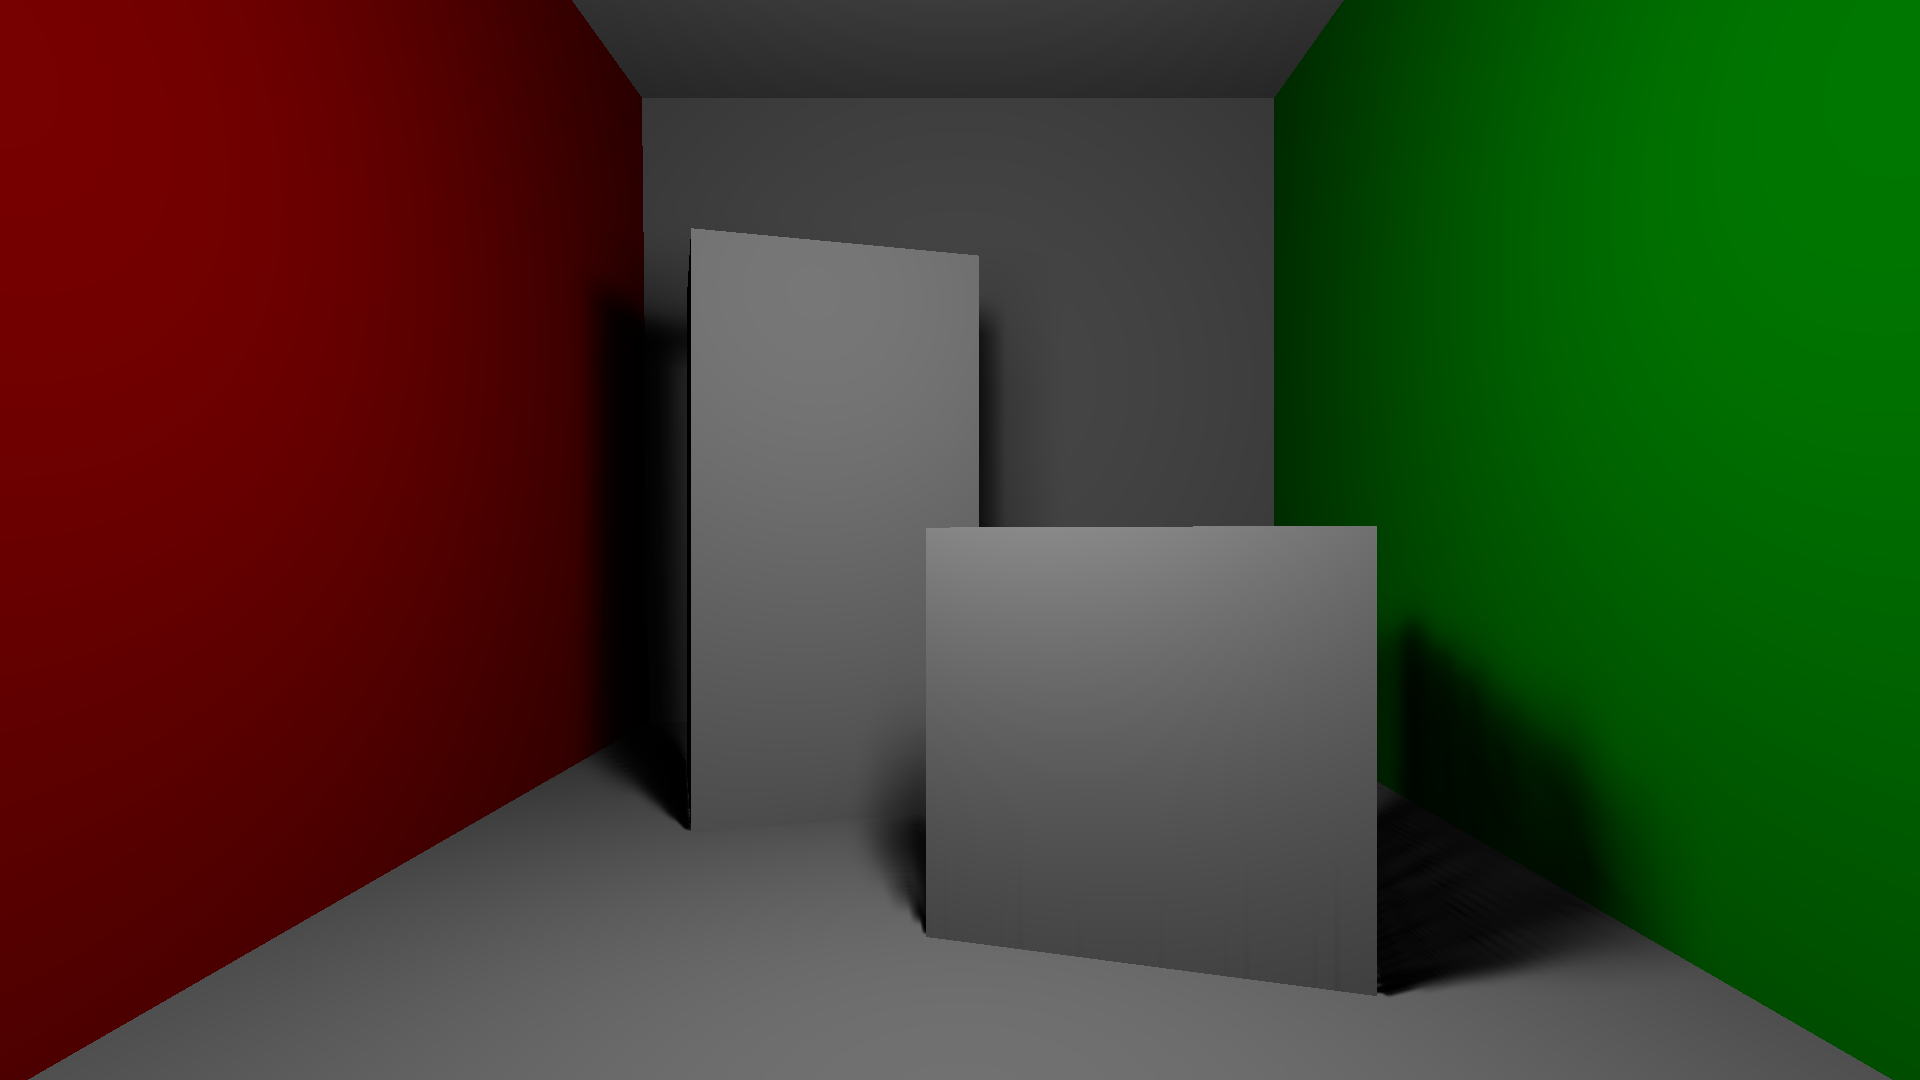
\includegraphics[width=\linewidth]{media/finals/cornell_direct.png}
	\end{subfigure}%
	\hspace{0.01\textwidth}
	\begin{subfigure}[t]{.49\linewidth}
		\centering
		\caption*{Indirecta}
		\captionsetup{justification=centering}
		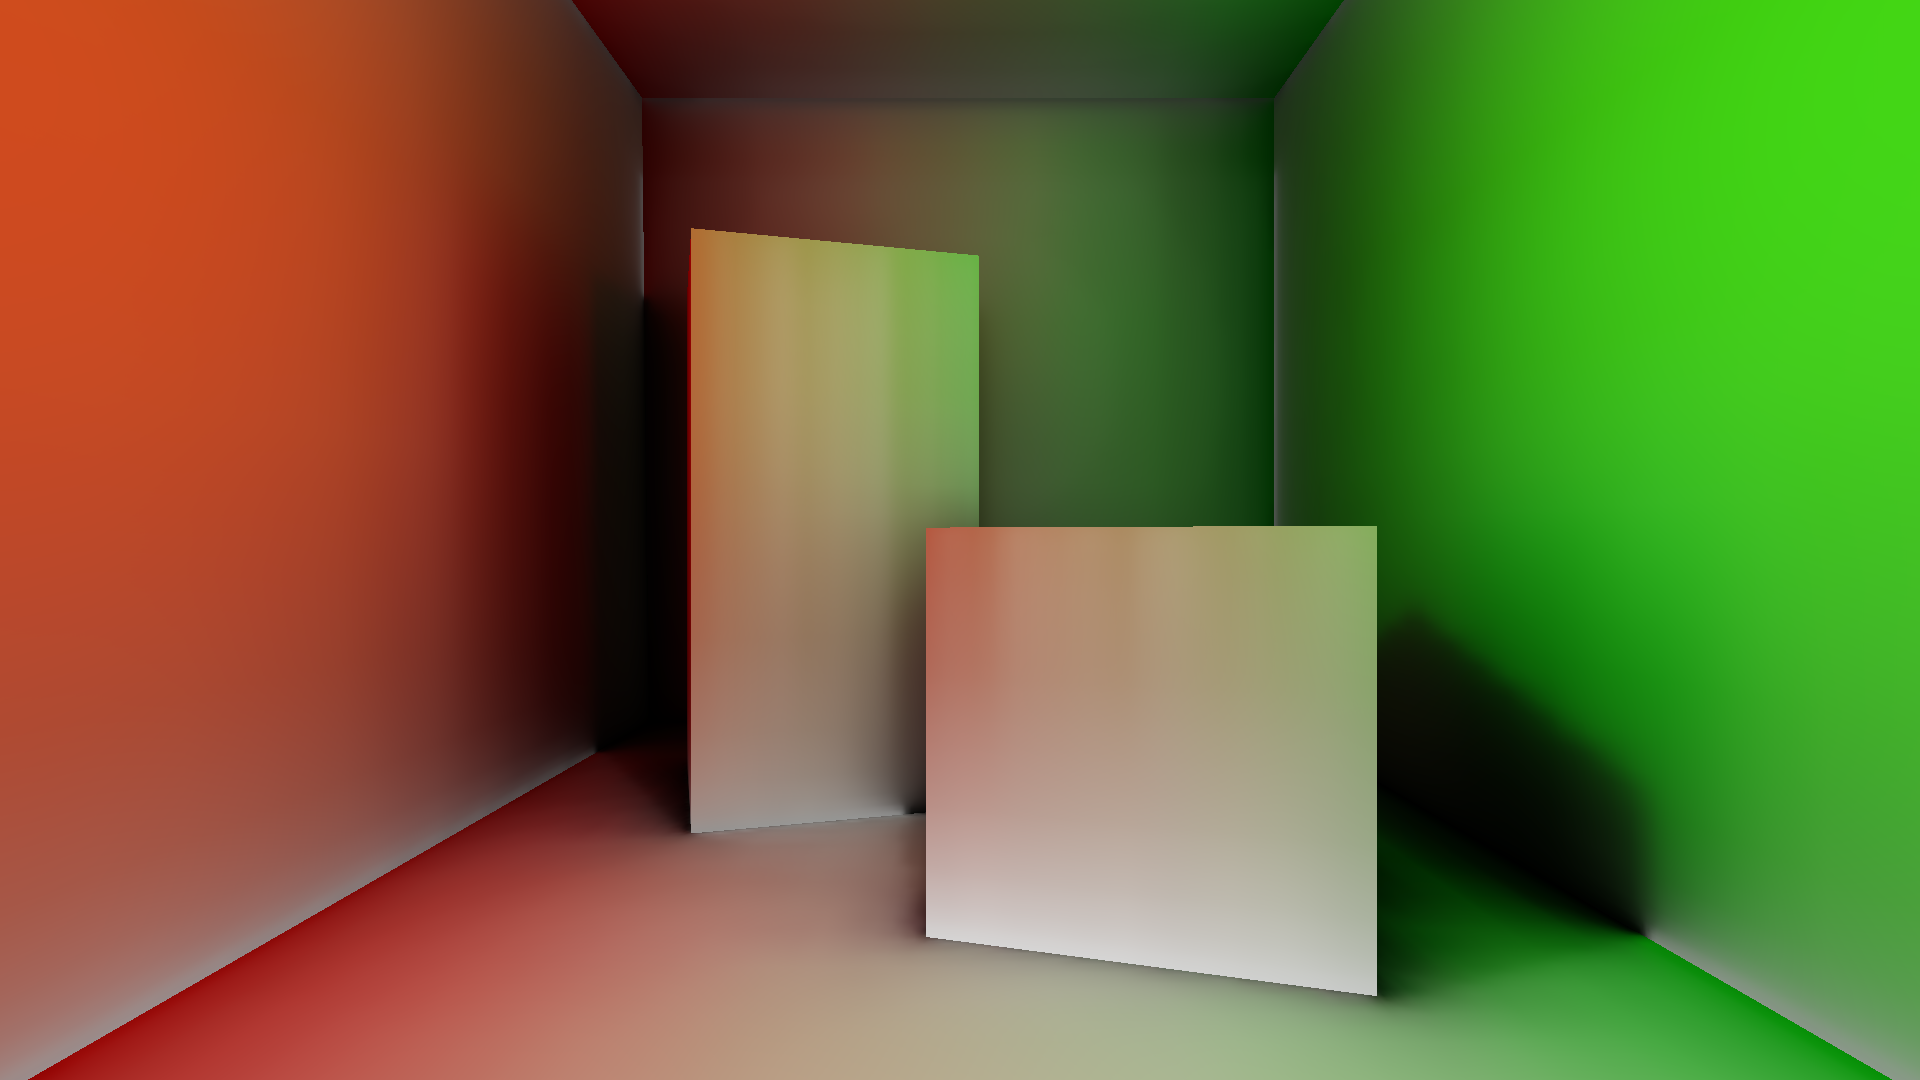
\includegraphics[width=\linewidth]{media/finals/cornell_indirect.png}
	\end{subfigure}%
	\par\smallskip
	\begin{subfigure}[t]{.49\linewidth}
		\centering
		\captionsetup{justification=centering}
		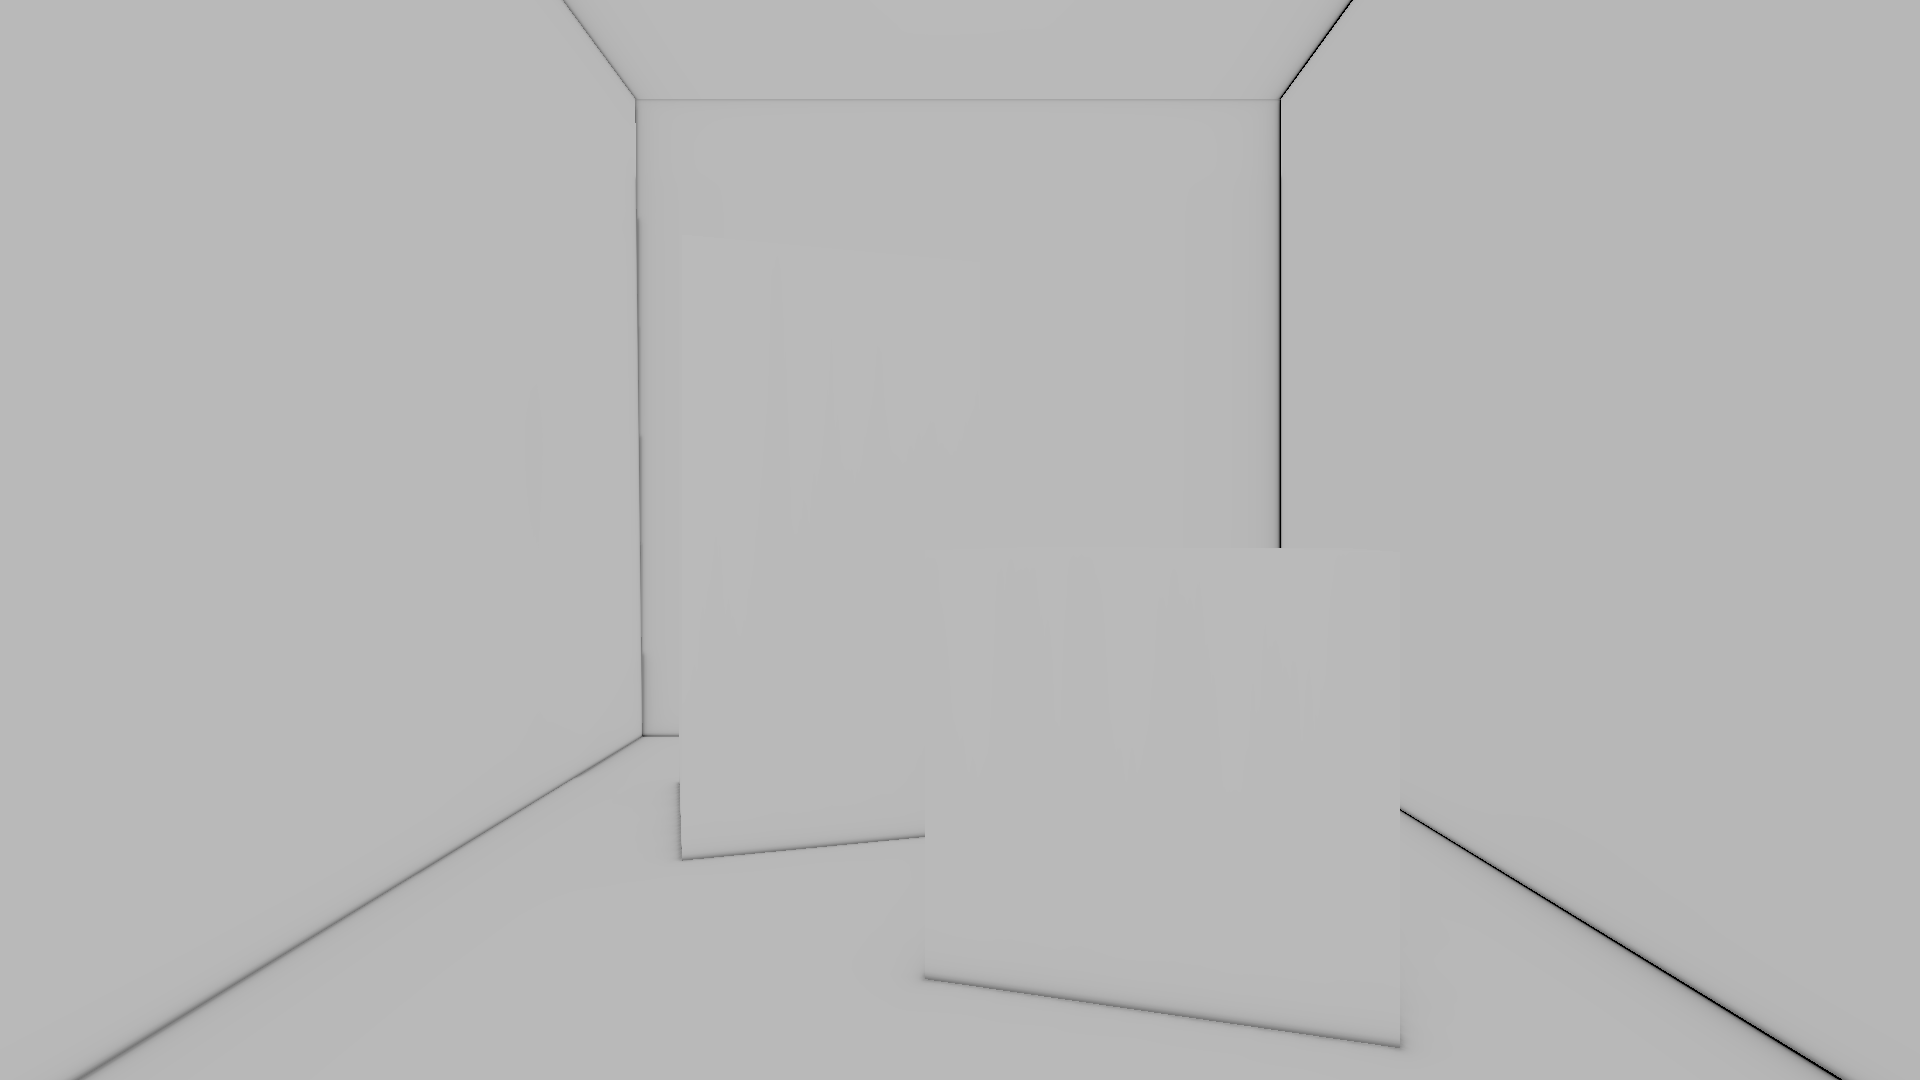
\includegraphics[width=\linewidth]{media/finals/cornell_ao.png}
		\caption*{Oclusión Ambiental}
	\end{subfigure}%
	\hspace{0.01\textwidth}
	\begin{subfigure}[t]{.49\linewidth}
		\centering
		\captionsetup{justification=centering}
		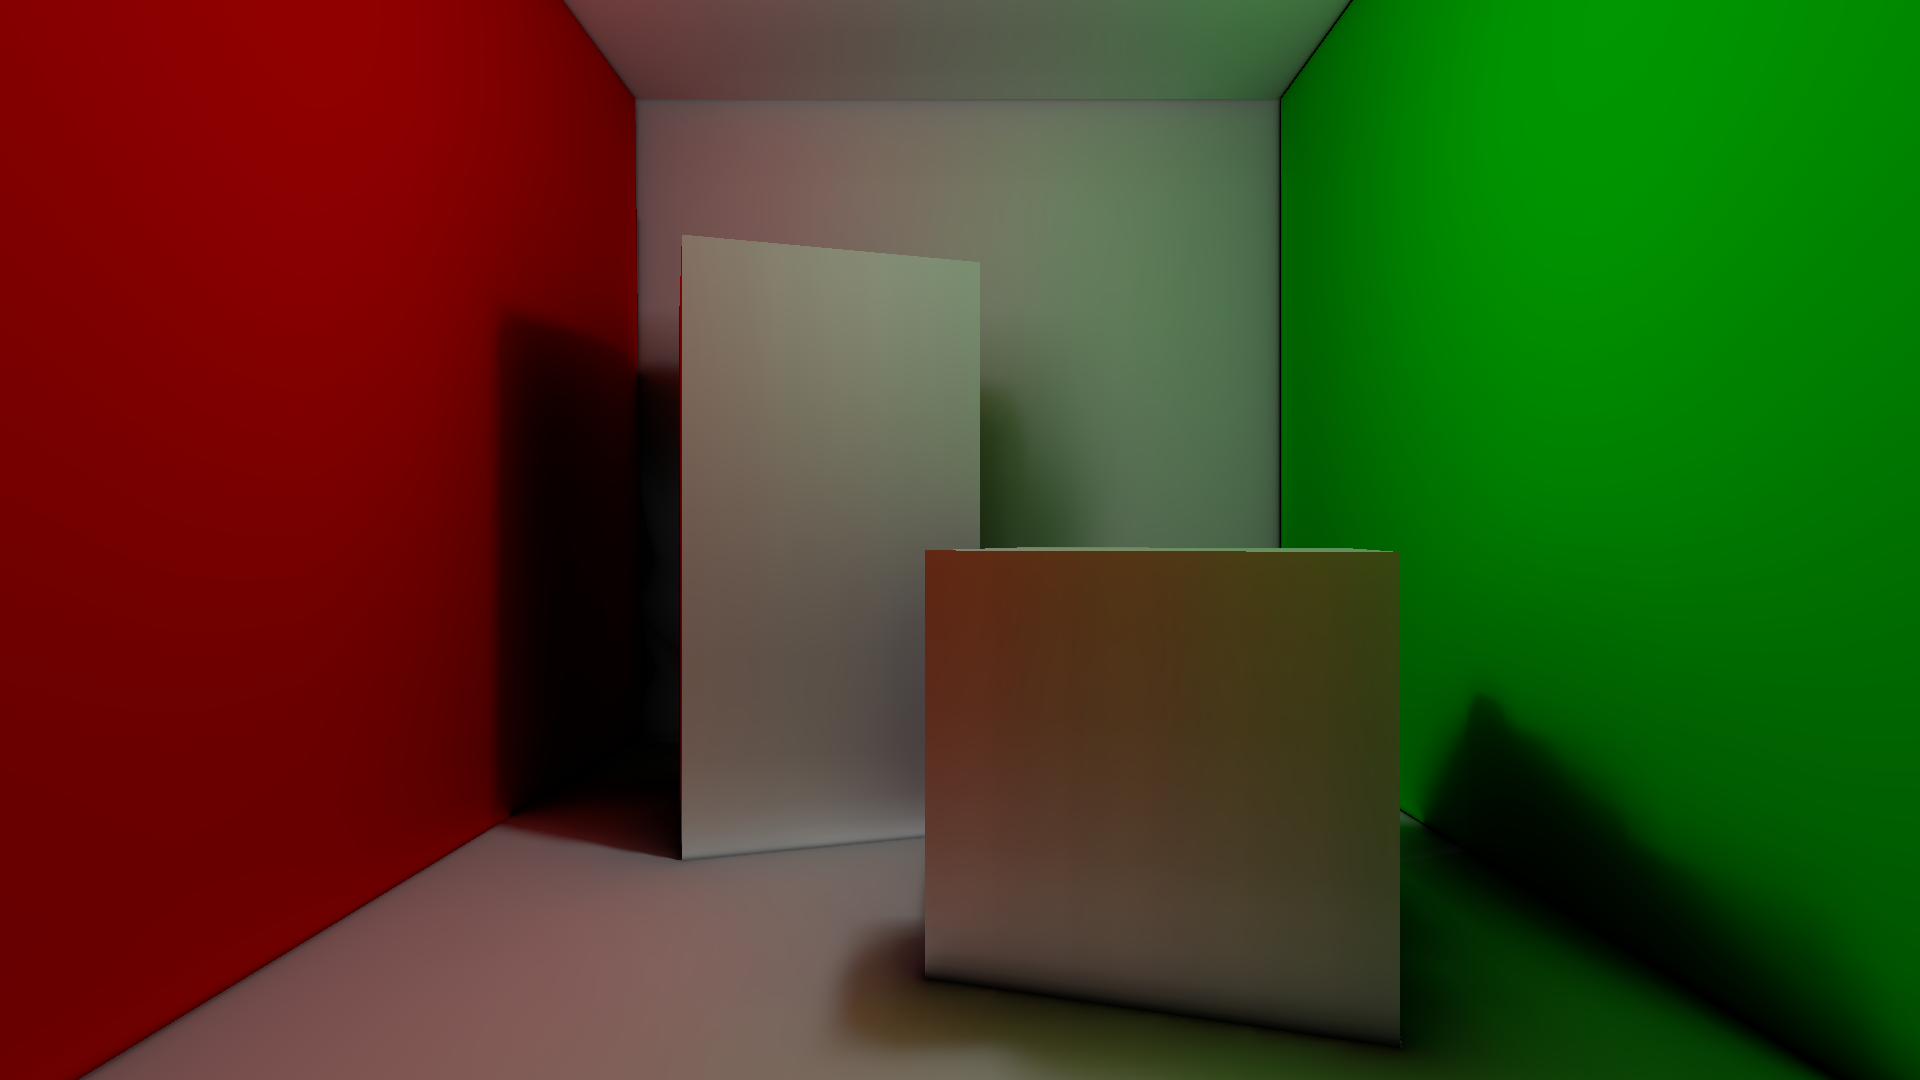
\includegraphics[width=\linewidth]{media/finals/cornell_gi.png}
		\caption*{Resultado: Directa, Indirecta y Oclusión Ambiental}
	\end{subfigure}%
	\caption{Composición para la escena Cornell Box.}
	\label{fig:cornell_final}
\end{figure}
\begin{figure}[H]
	\centering
	\begin{subfigure}[t]{.49\linewidth}
		\centering
		\captionsetup{justification=centering}
		% \caption*{Directa}
		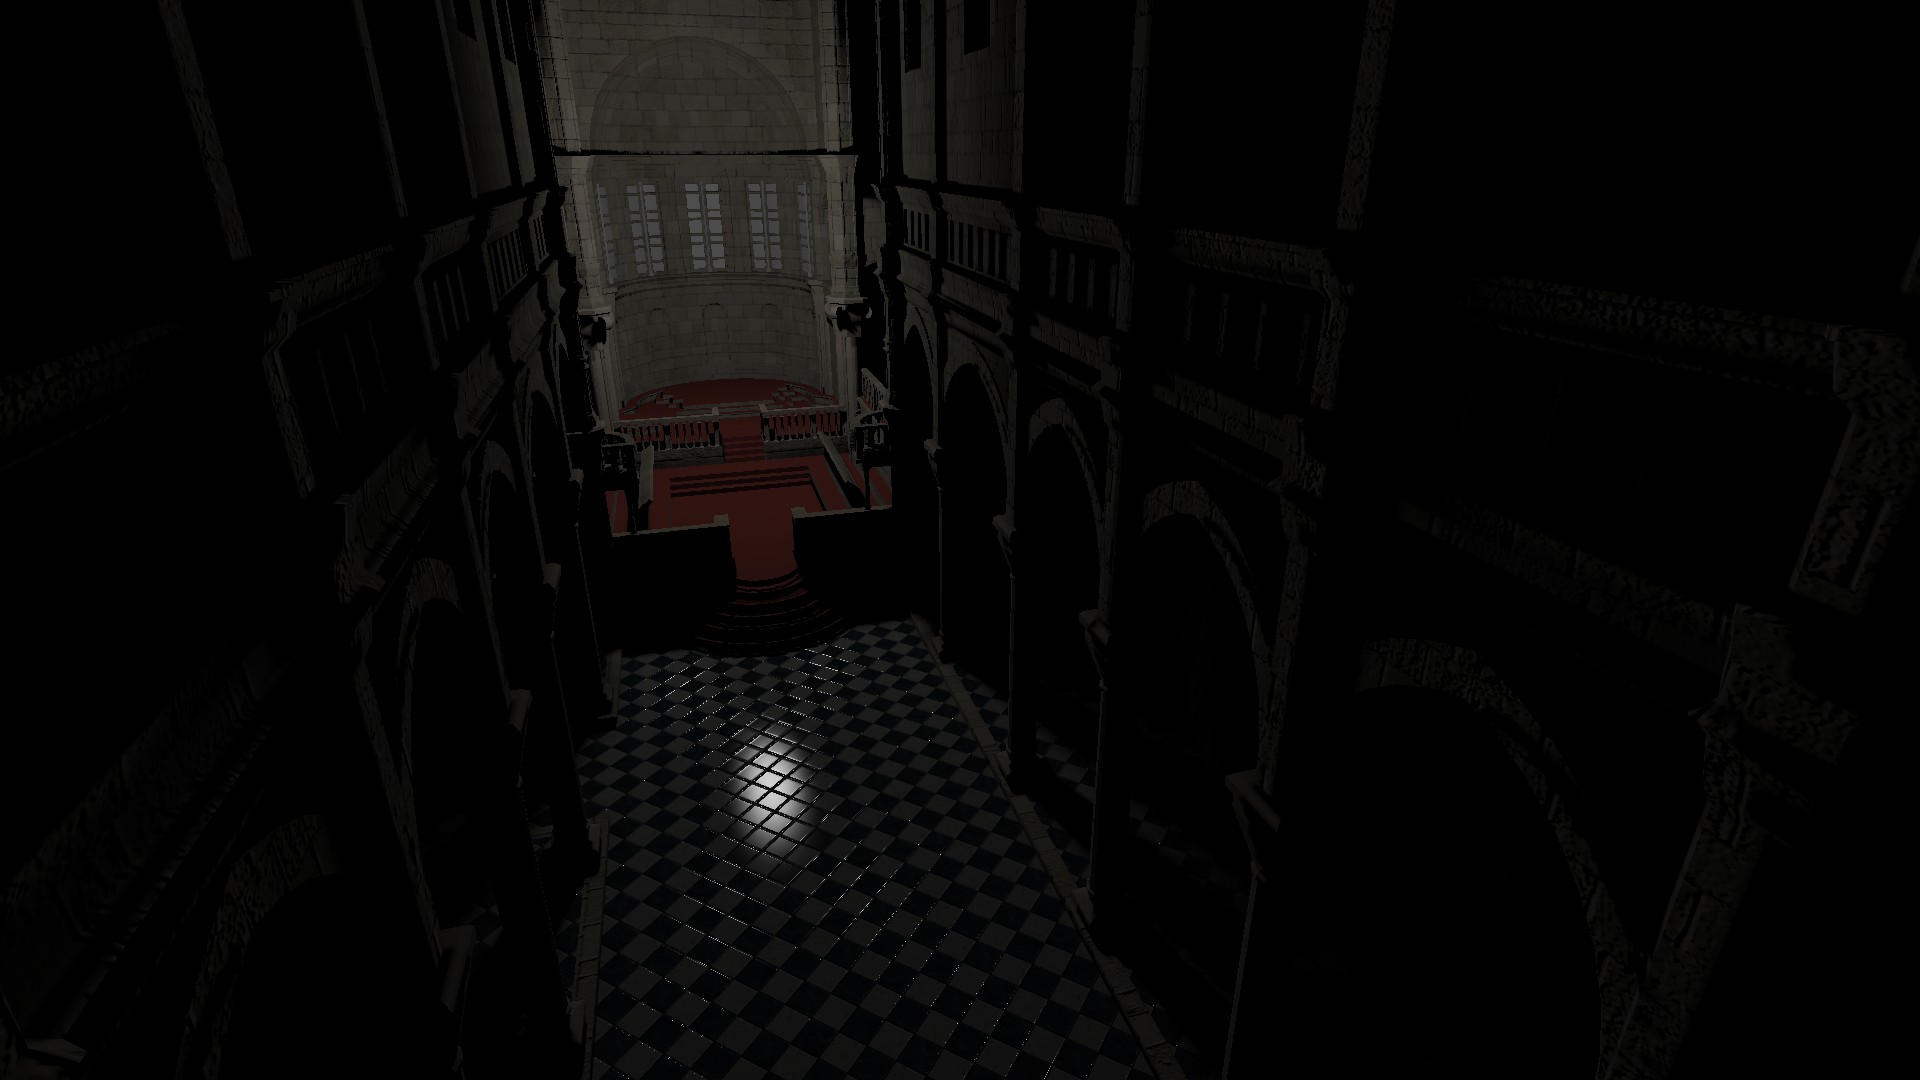
\includegraphics[width=\linewidth]{media/finals/sibenik_direct.png}
	\end{subfigure}%
	\hspace{0.01\textwidth}
	\begin{subfigure}[t]{.49\linewidth}
		\centering
		% \caption*{Indirecta}
		\captionsetup{justification=centering}
		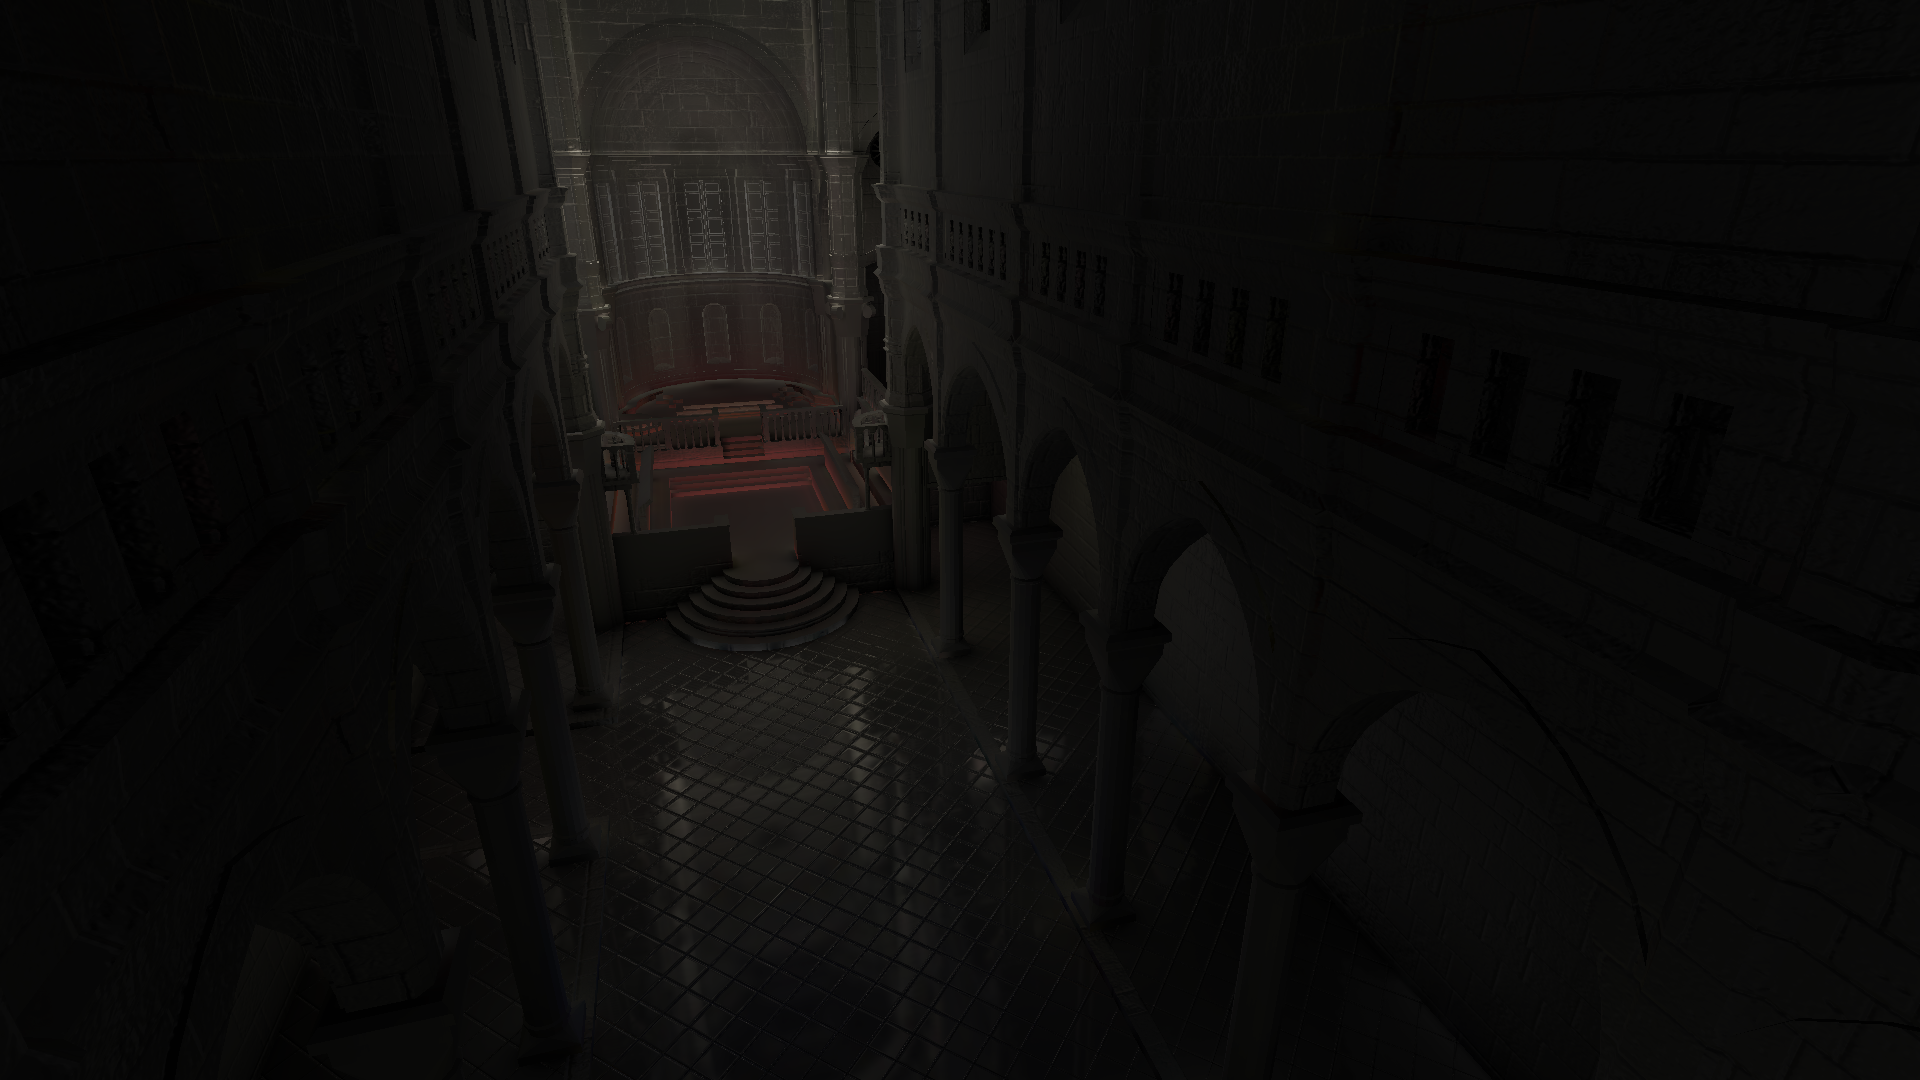
\includegraphics[width=\linewidth]{media/finals/sibenik_indirect.png}
	\end{subfigure}%
	\par\smallskip
	\begin{subfigure}[t]{.49\linewidth}
		\centering
		% \caption*{Oclusión Ambiental}
		\captionsetup{justification=centering}
		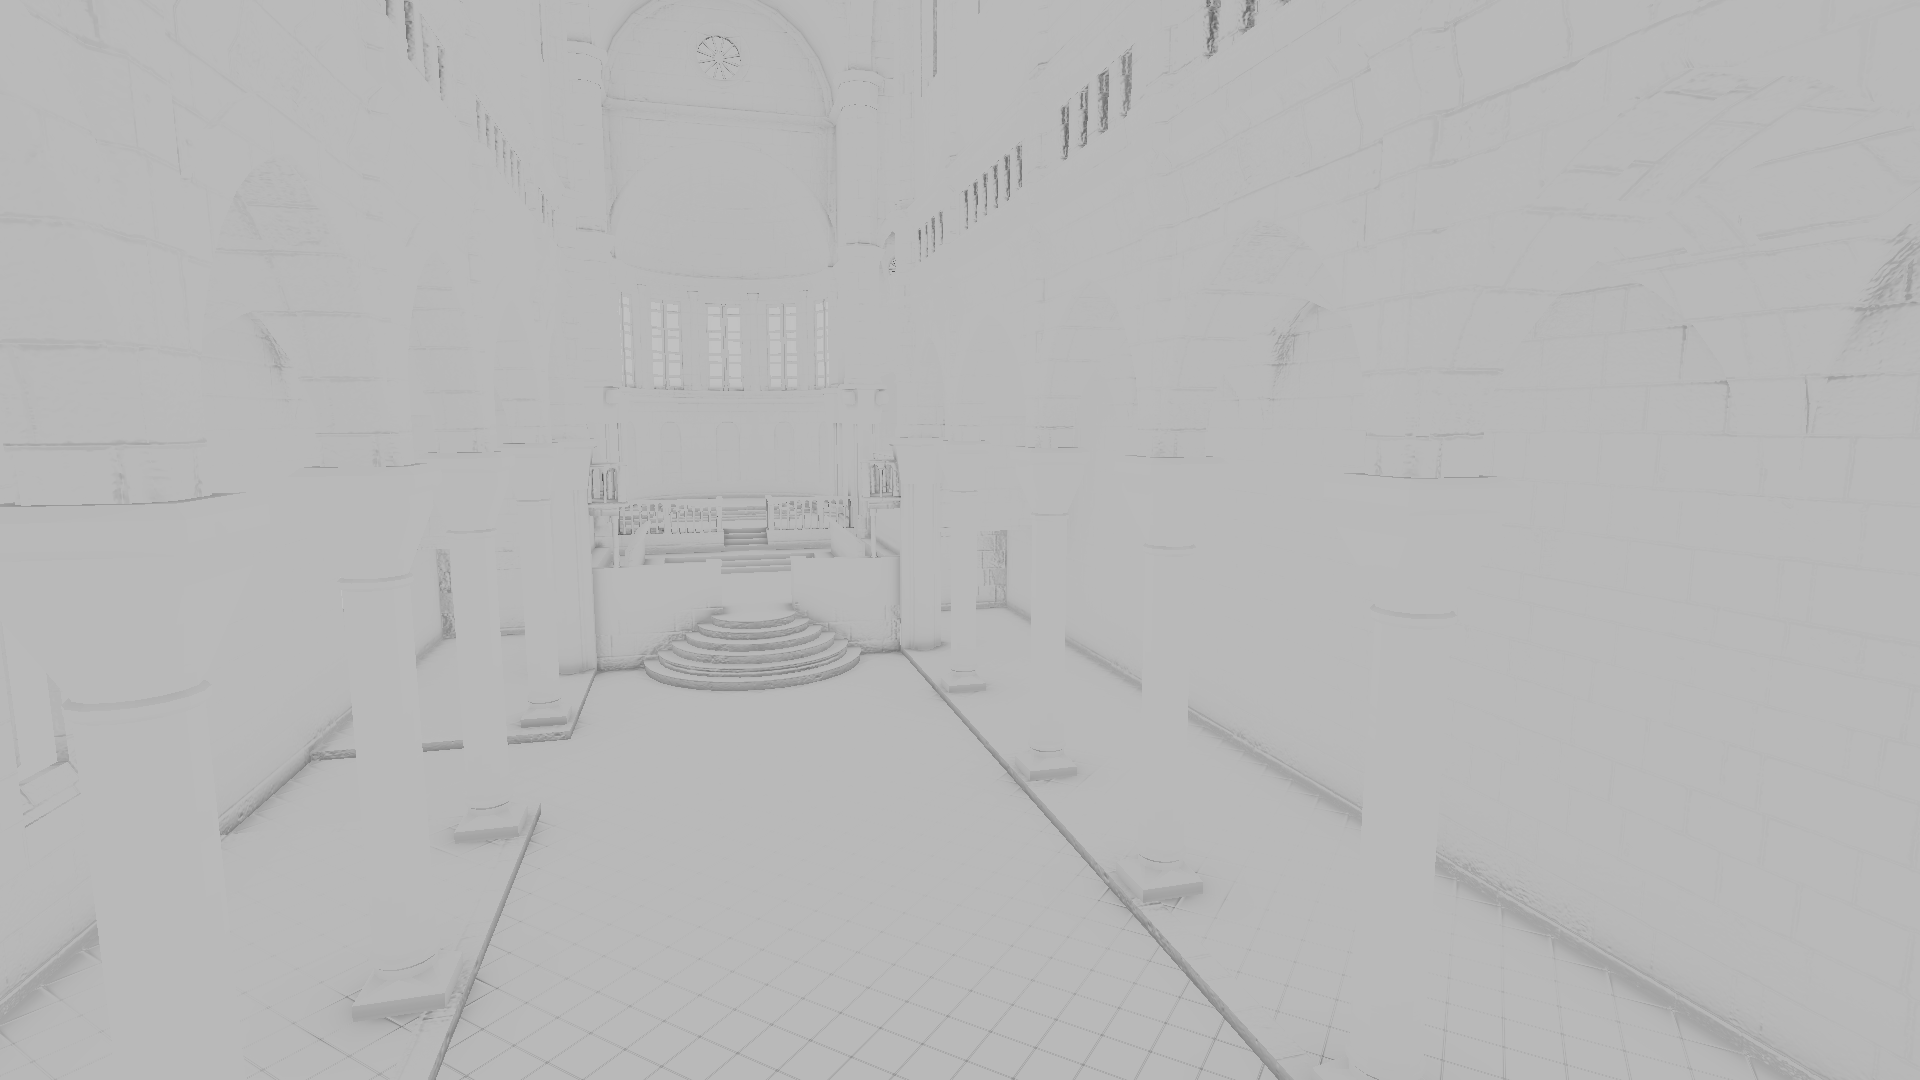
\includegraphics[width=\linewidth]{media/finals/sibenik_ao.png}
	\end{subfigure}%
	\hspace{0.01\textwidth}
	\begin{subfigure}[t]{.49\linewidth}
		\centering
		% \caption*{Directa + Indirecta + Oclusión Ambiental}
		\captionsetup{justification=centering}
		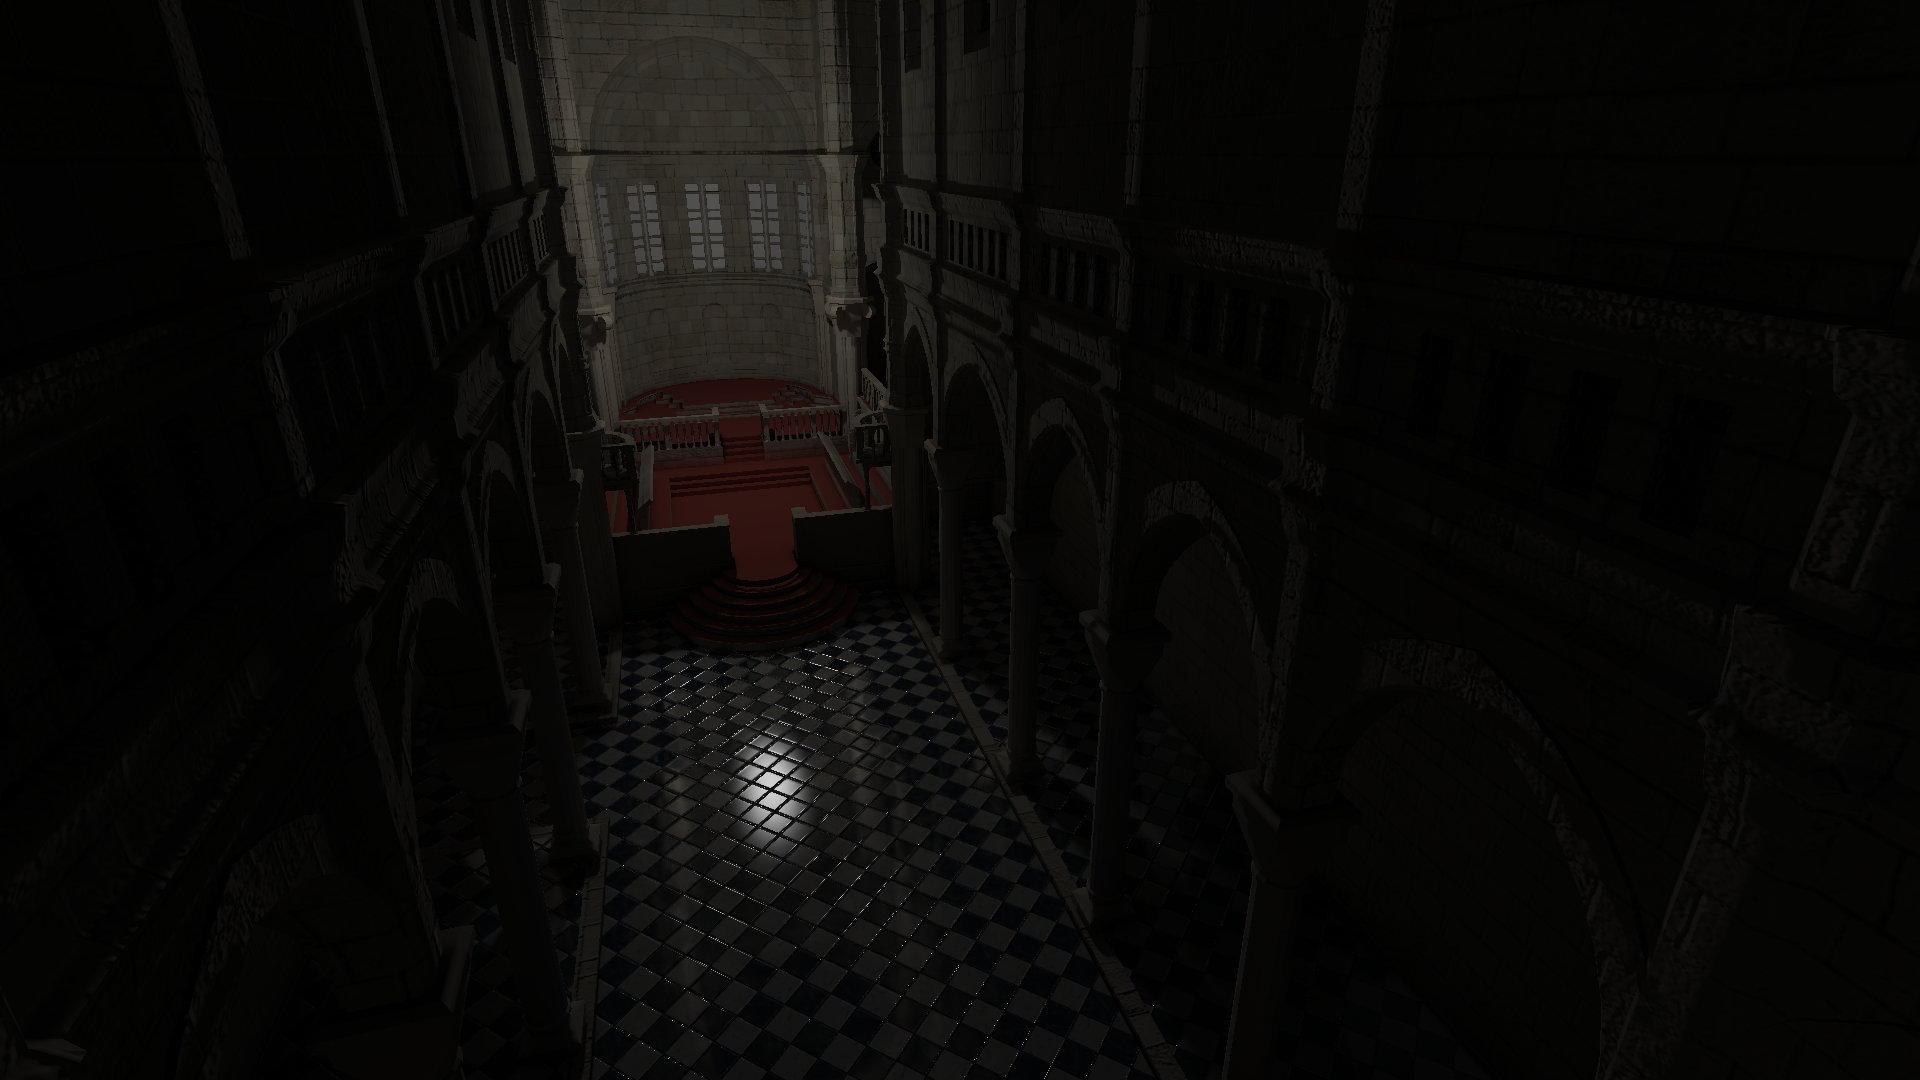
\includegraphics[width=\linewidth]{media/finals/sibenik_gi.png}
	\end{subfigure}%
	\caption{Composición para la escena Sibenik.}
	\label{fig:sibenik_final}
\end{figure}
\begin{figure}[H]
	\centering
	\begin{subfigure}[t]{.49\linewidth}
		\centering
		\captionsetup{justification=centering}
		% \caption*{Directa}
		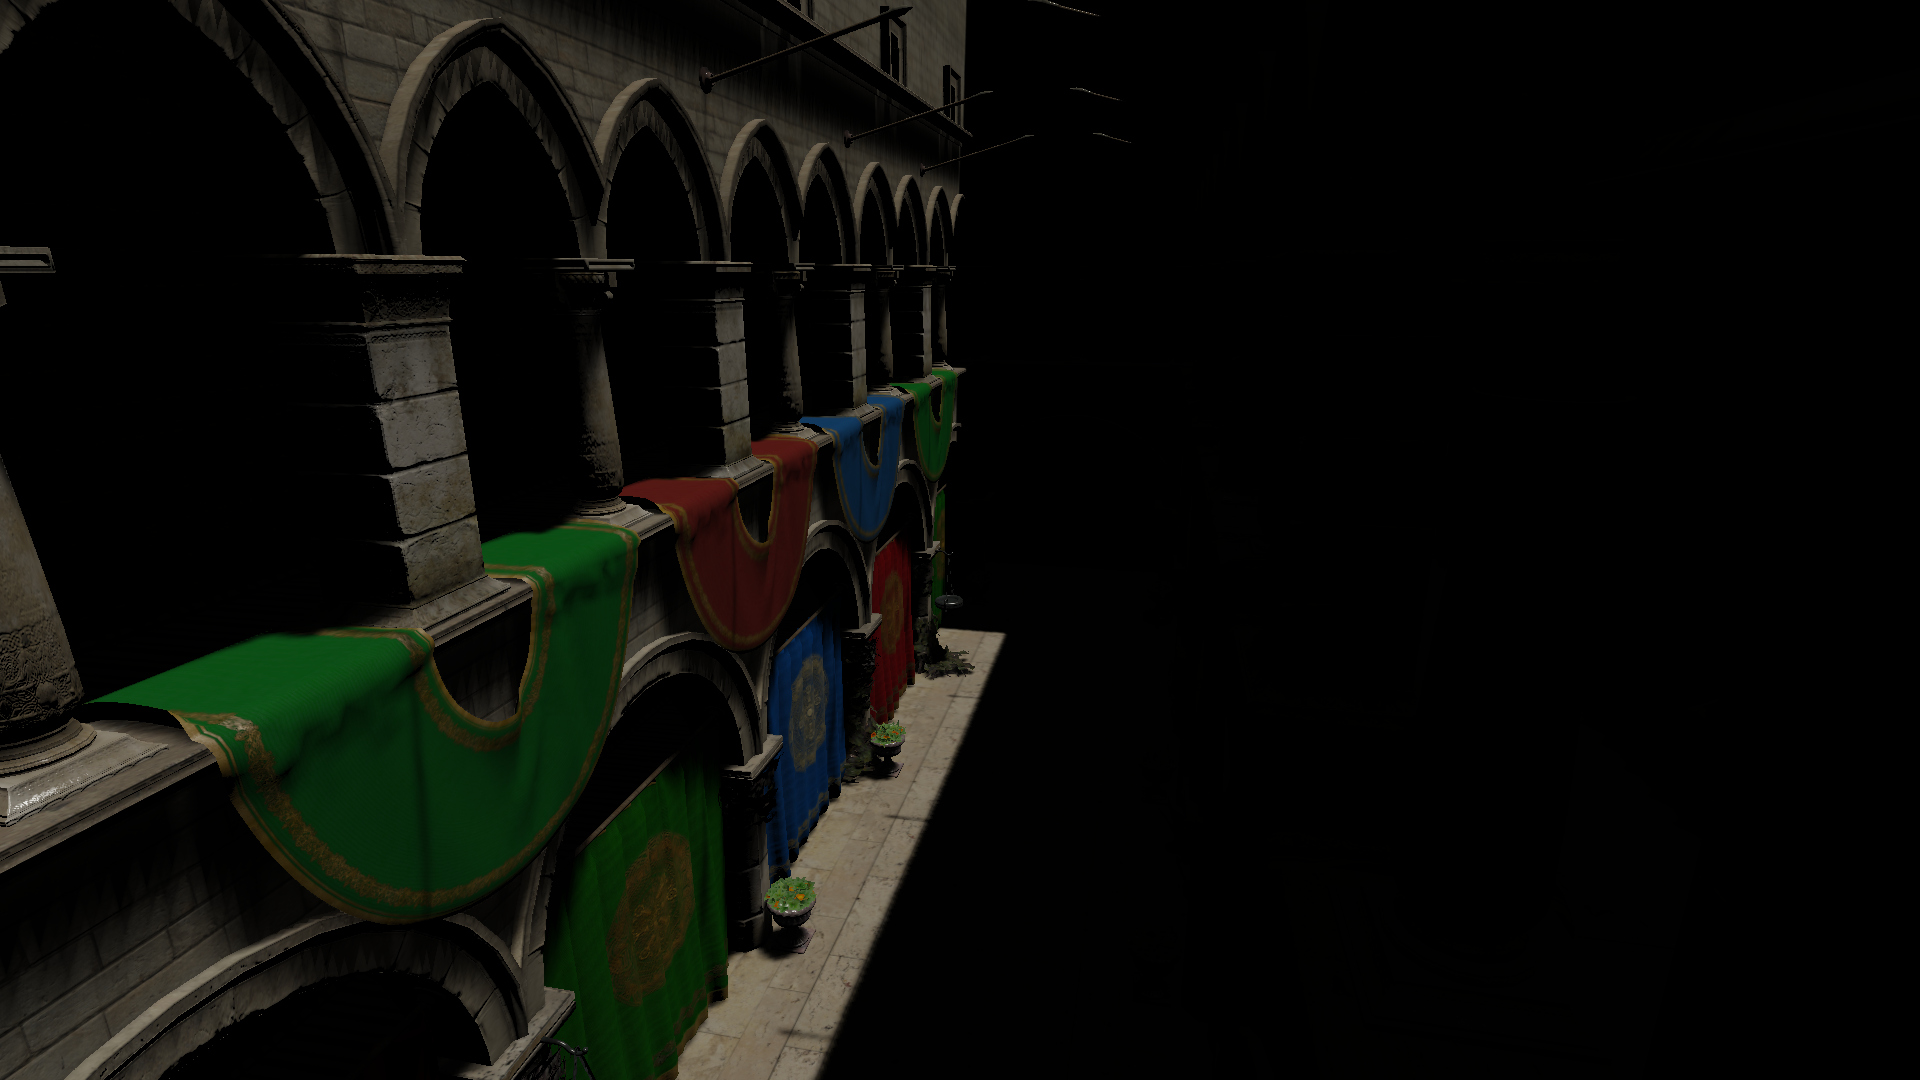
\includegraphics[width=\linewidth]{media/finals/sponza_direct.png}
	\end{subfigure}%
	\hspace{0.01\textwidth}
	\begin{subfigure}[t]{.49\linewidth}
		\centering
		% \caption*{Indirecta}
		\captionsetup{justification=centering}
		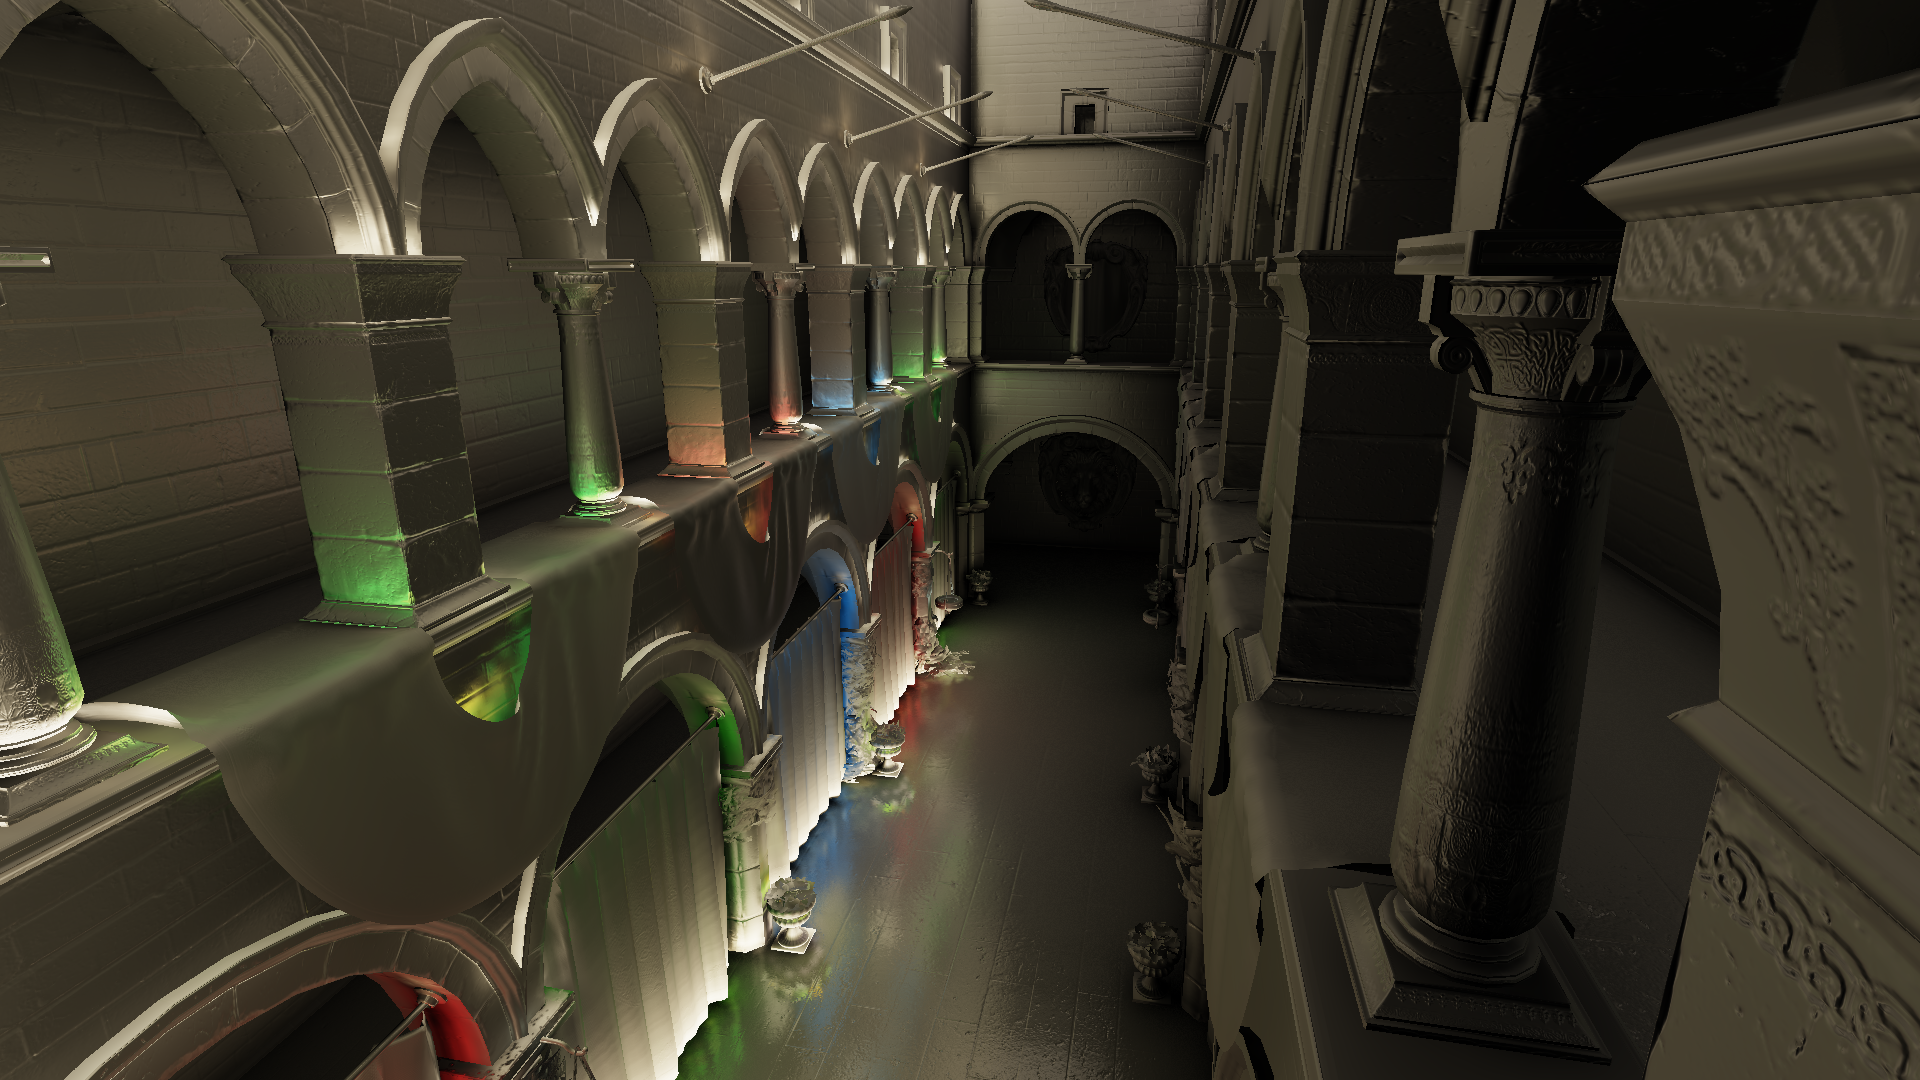
\includegraphics[width=\linewidth]{media/finals/sponza_indirect.png}
	\end{subfigure}%
	\par\smallskip
	\begin{subfigure}[t]{.49\linewidth}
		\centering
		% \caption*{Oclusión Ambiental}
		\captionsetup{justification=centering}
		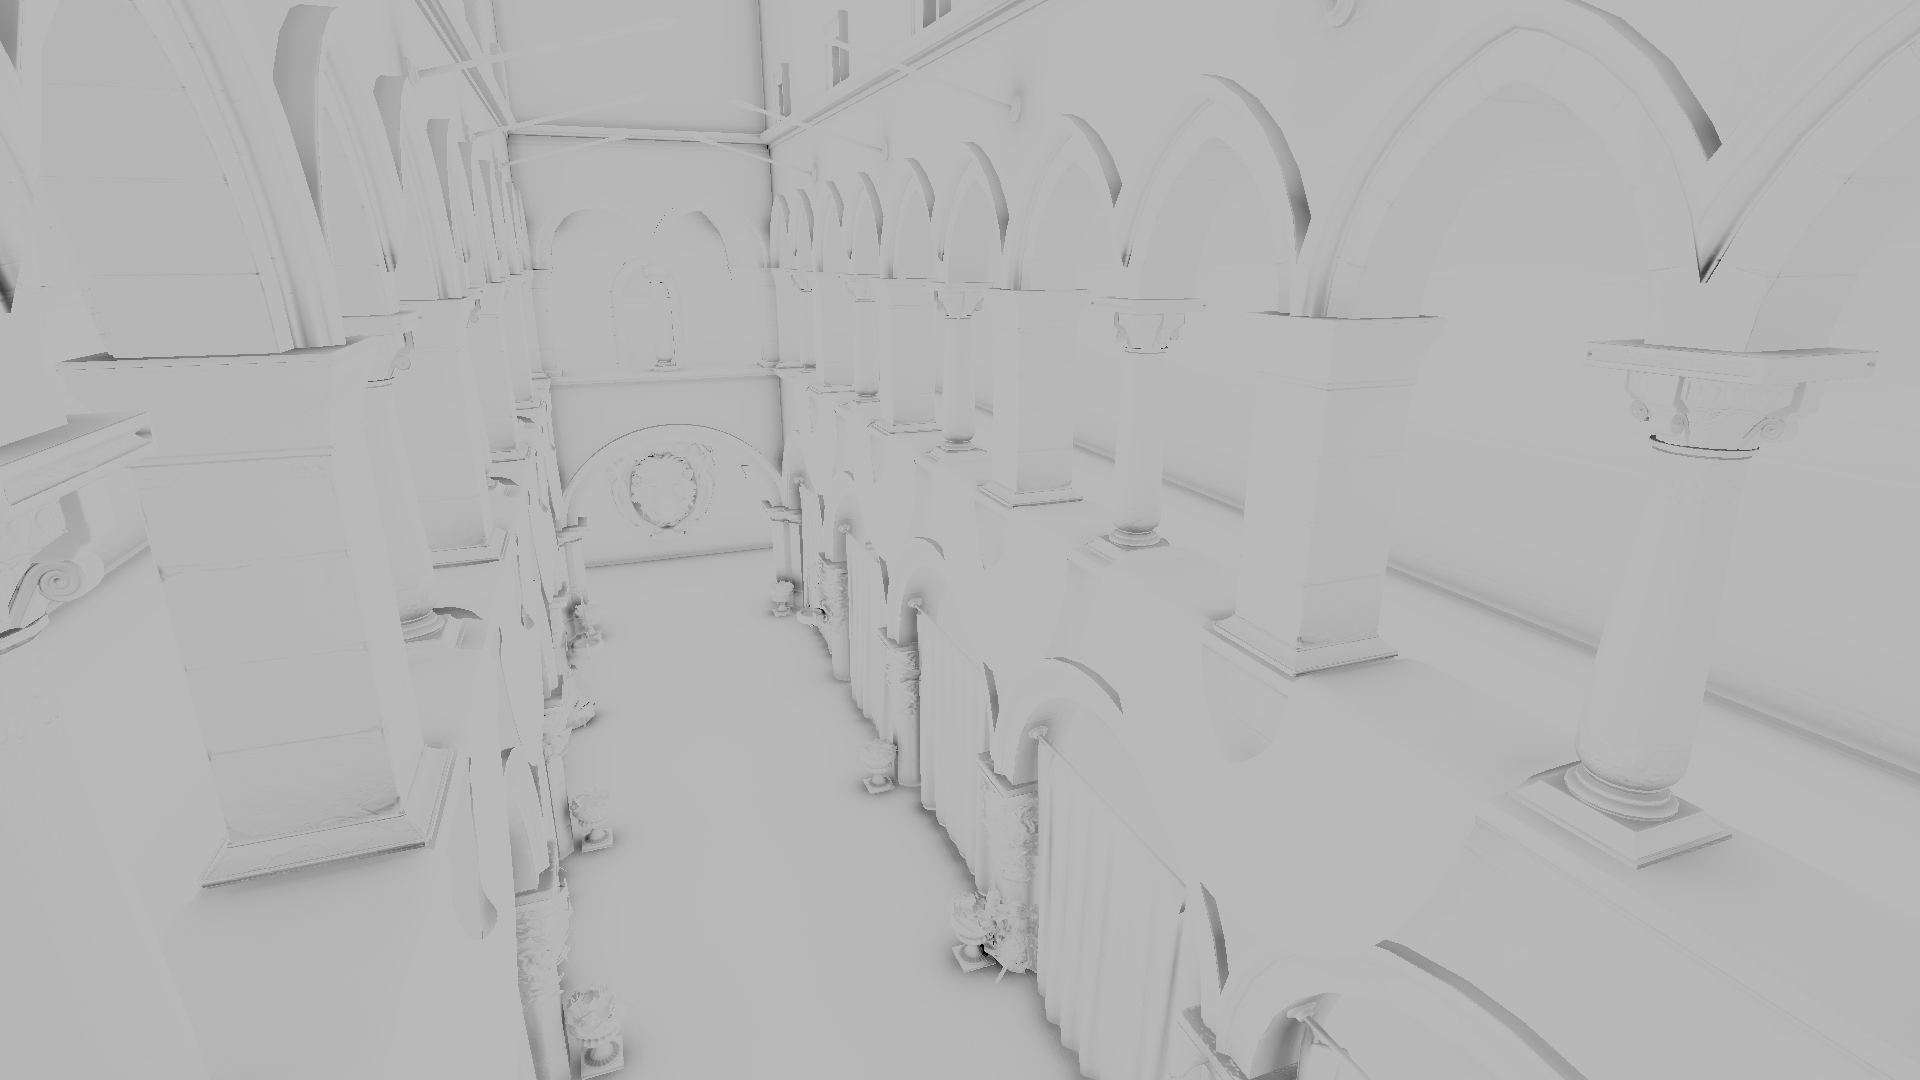
\includegraphics[width=\linewidth]{media/finals/sponza_ao.png}
	\end{subfigure}%
	\hspace{0.01\textwidth}
	\begin{subfigure}[t]{.49\linewidth}
		\centering
		% \caption*{Directa + Indirecta + Oclusión Ambiental}
		\captionsetup{justification=centering}
		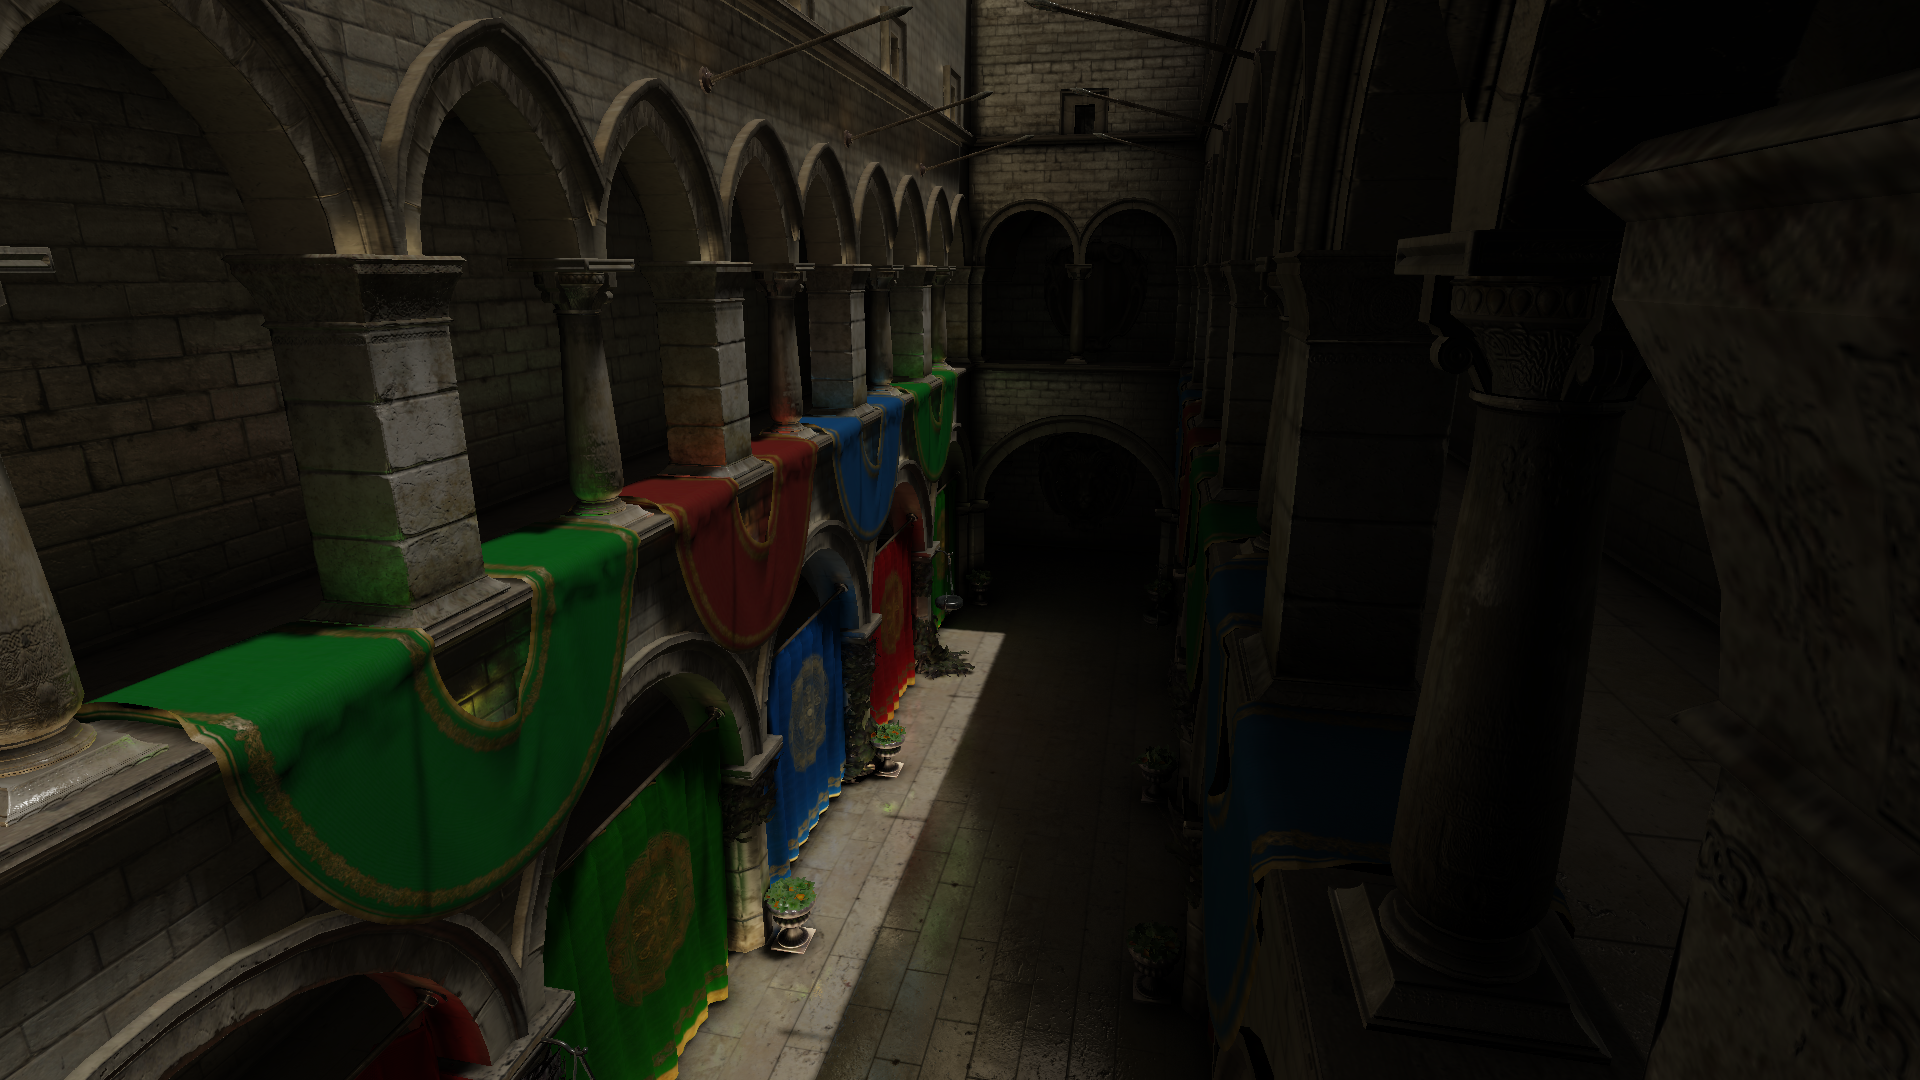
\includegraphics[width=\linewidth]{media/finals/sponza_gi.png}
	\end{subfigure}%
	\caption{Composición para la escena Sponza.}
	\label{fig:sponza_final}
\end{figure}
\begin{figure}[H]
	\centering
	\begin{subfigure}[t]{.49\linewidth}
		\centering
		\captionsetup{justification=centering}
		% \caption*{Directa}
		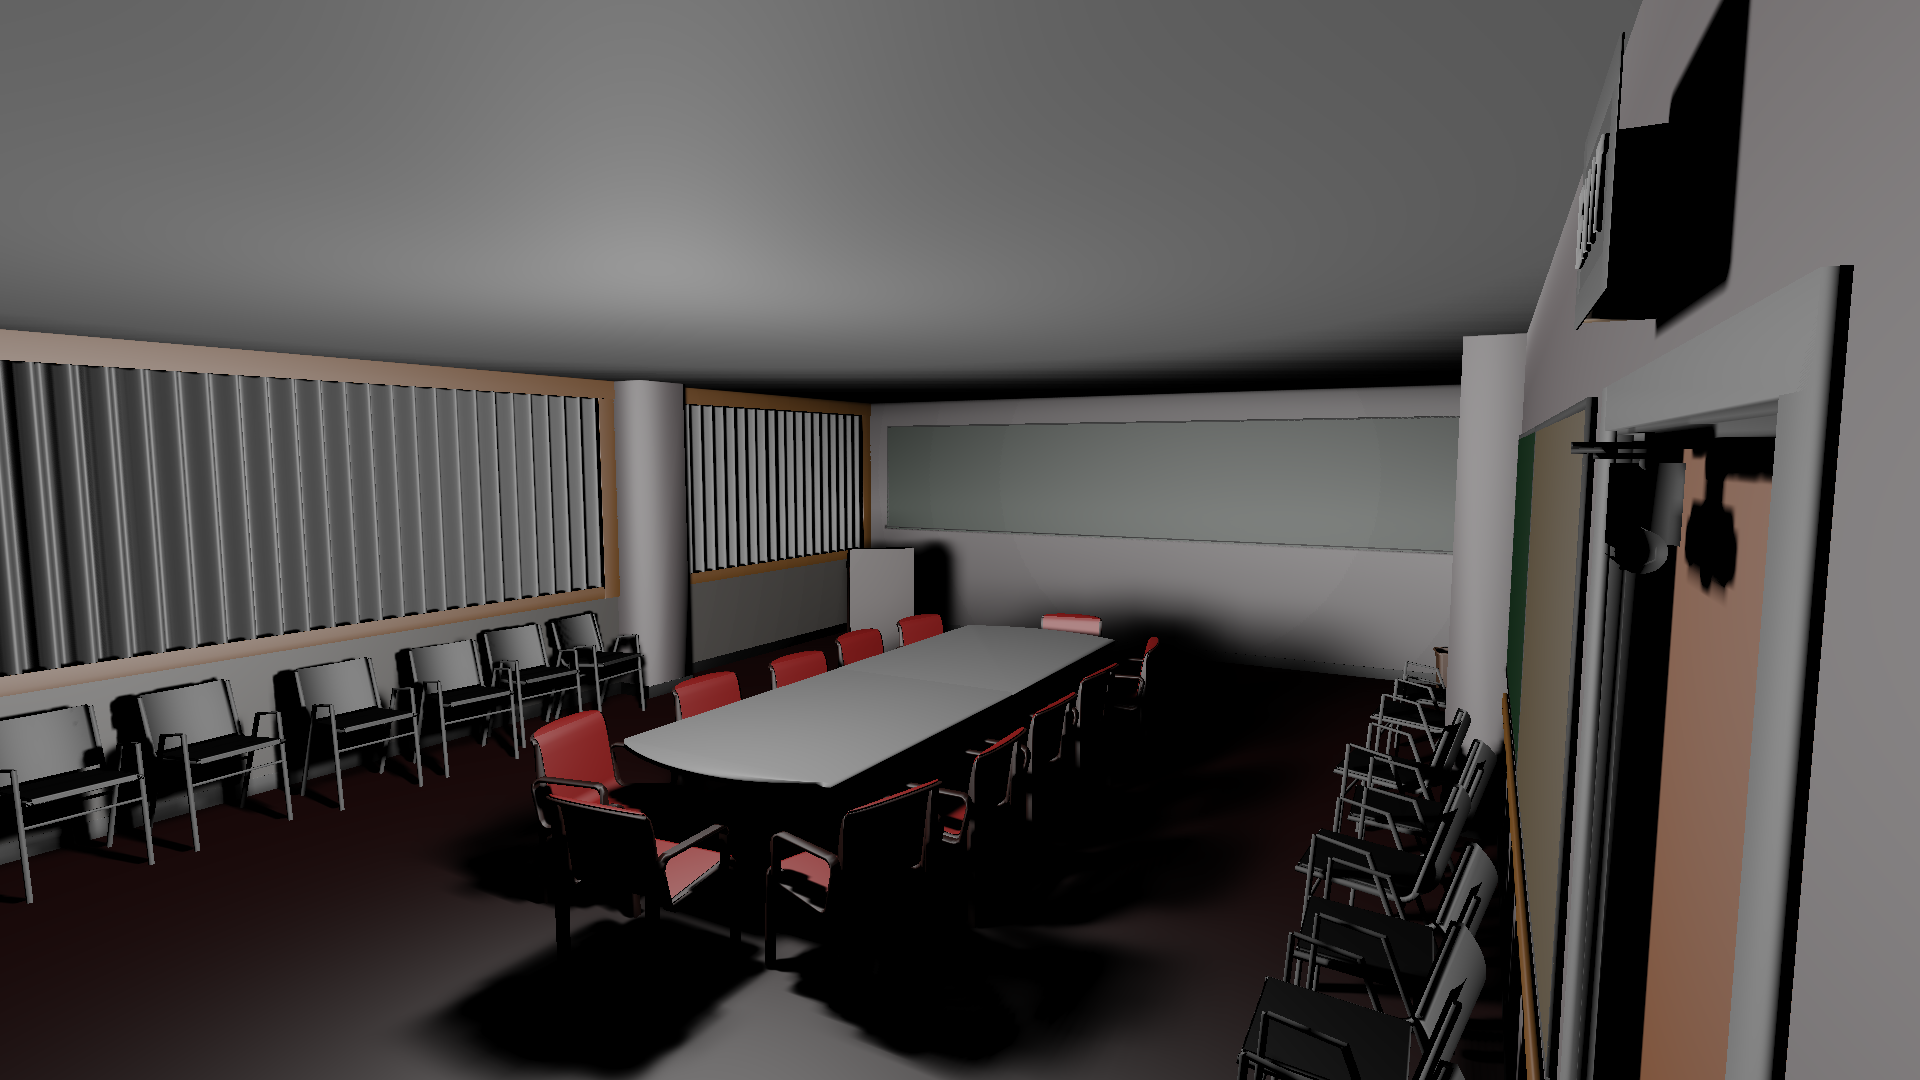
\includegraphics[width=\linewidth]{media/finals/conf_direct.png}
	\end{subfigure}%
	\hspace{0.01\textwidth}
	\begin{subfigure}[t]{.49\linewidth}
		\centering
		% \caption*{Indirecta}
		\captionsetup{justification=centering}
		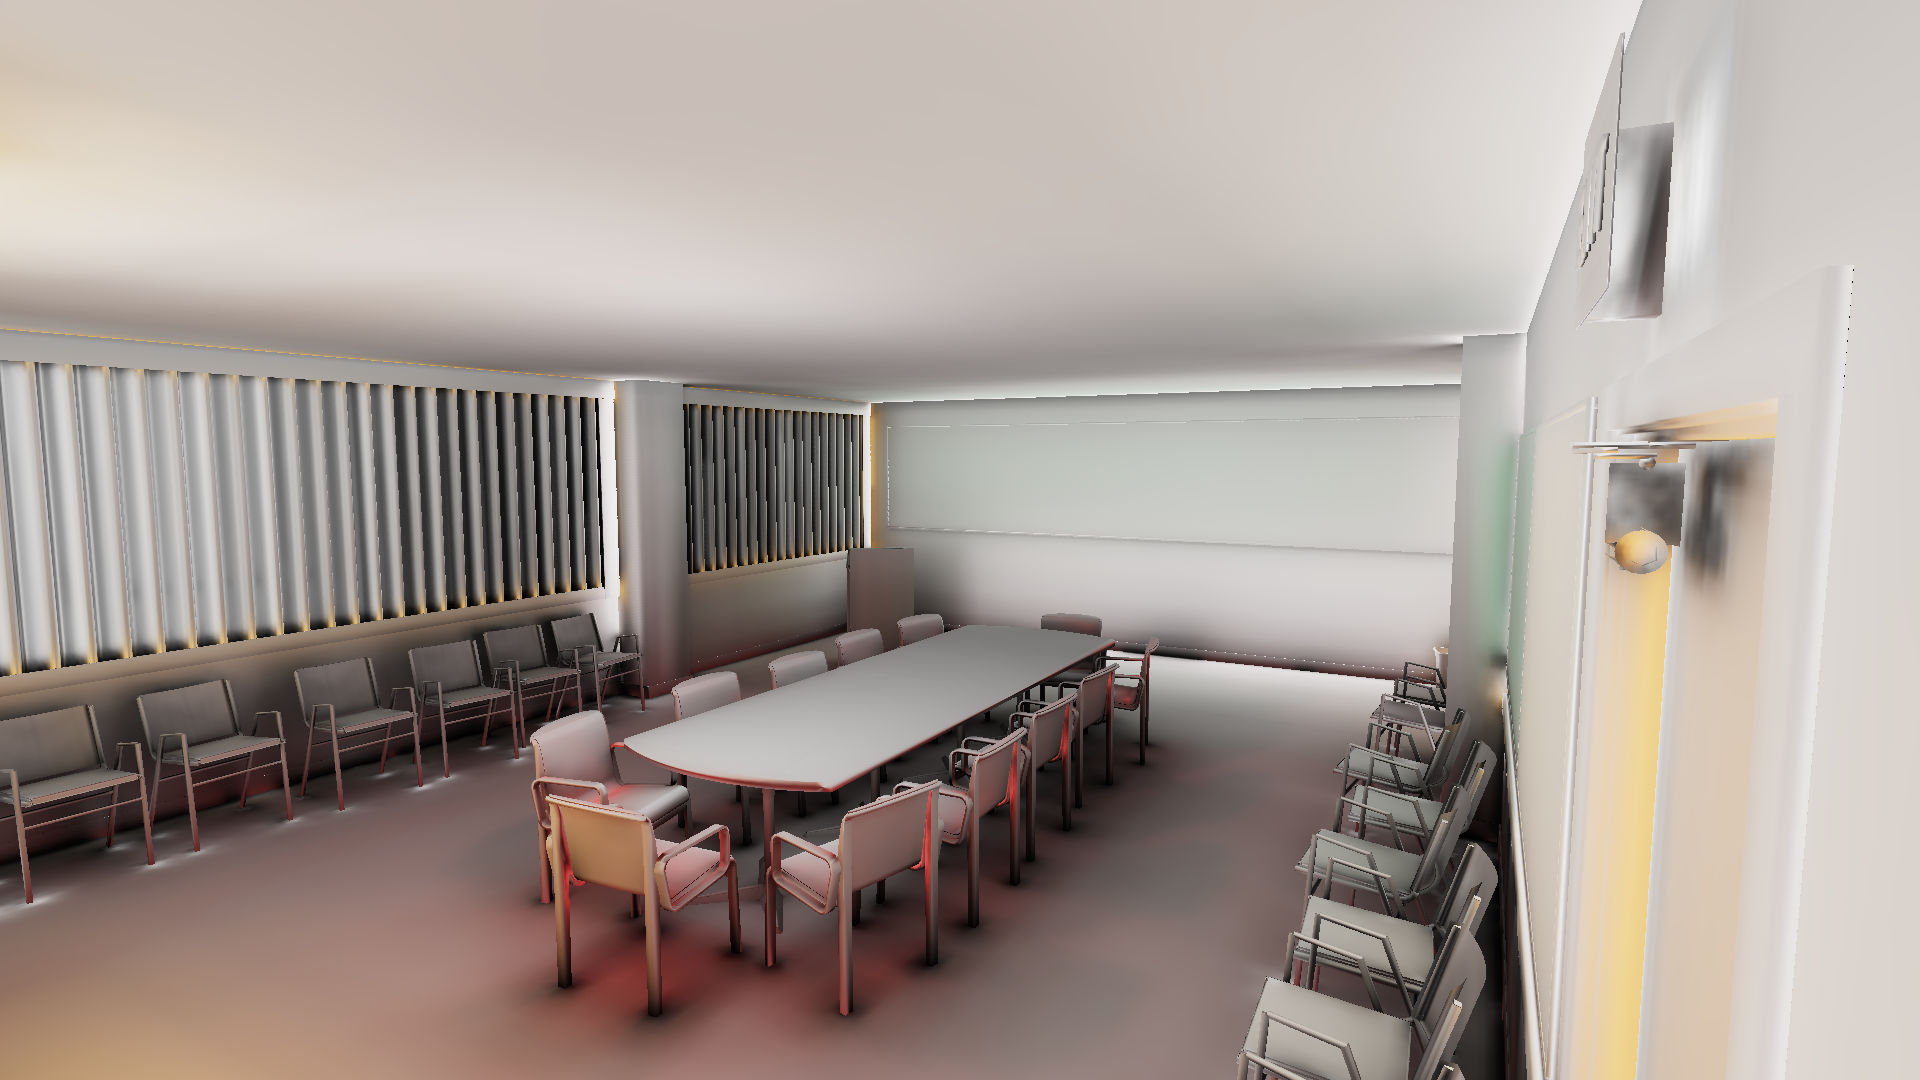
\includegraphics[width=\linewidth]{media/finals/conf_indirect.png}
	\end{subfigure}%
	\par\smallskip
	\begin{subfigure}[t]{.49\linewidth}
		\centering
		% \caption*{Oclusión Ambiental}
		\captionsetup{justification=centering}
		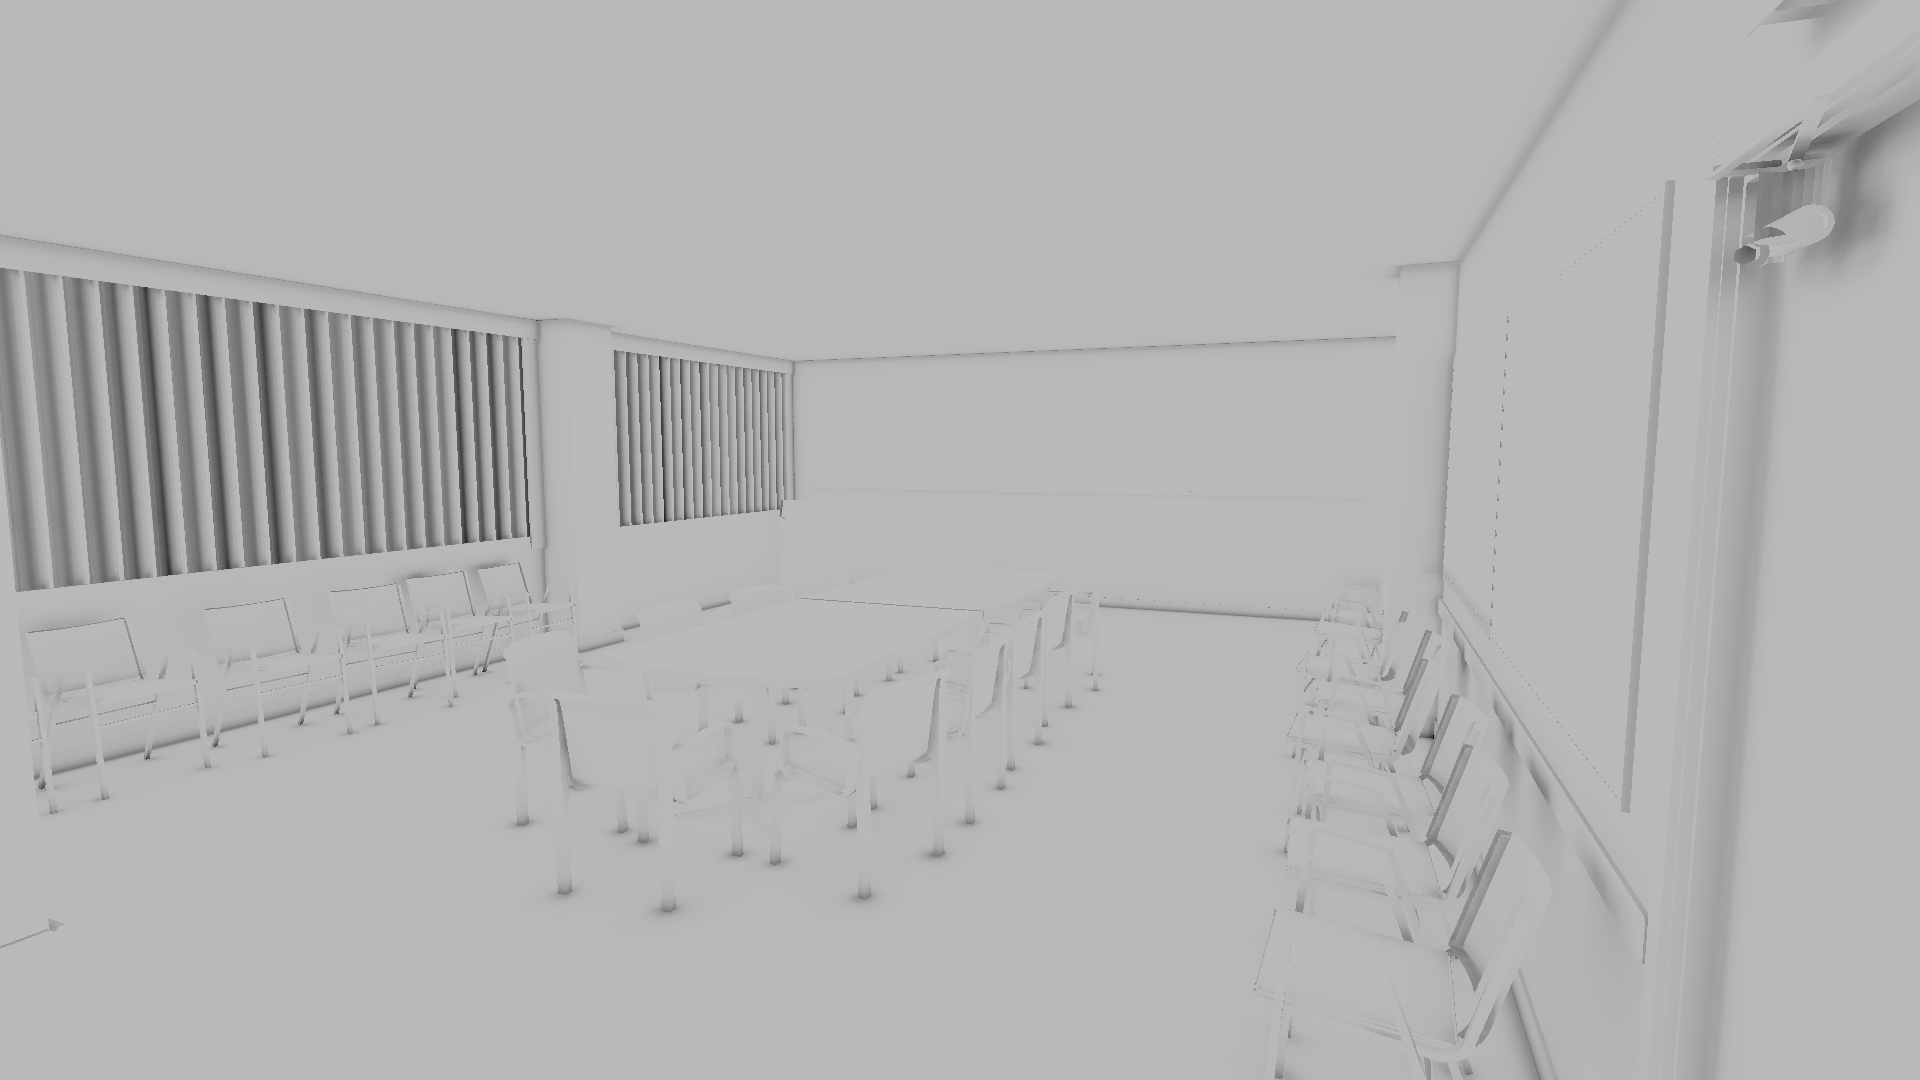
\includegraphics[width=\linewidth]{media/finals/conf_ao.png}
	\end{subfigure}%
	\hspace{0.01\textwidth}
	\begin{subfigure}[t]{.49\linewidth}
		\centering
		% \caption*{Directa + Indirecta + Oclusión Ambiental}
		\captionsetup{justification=centering}
		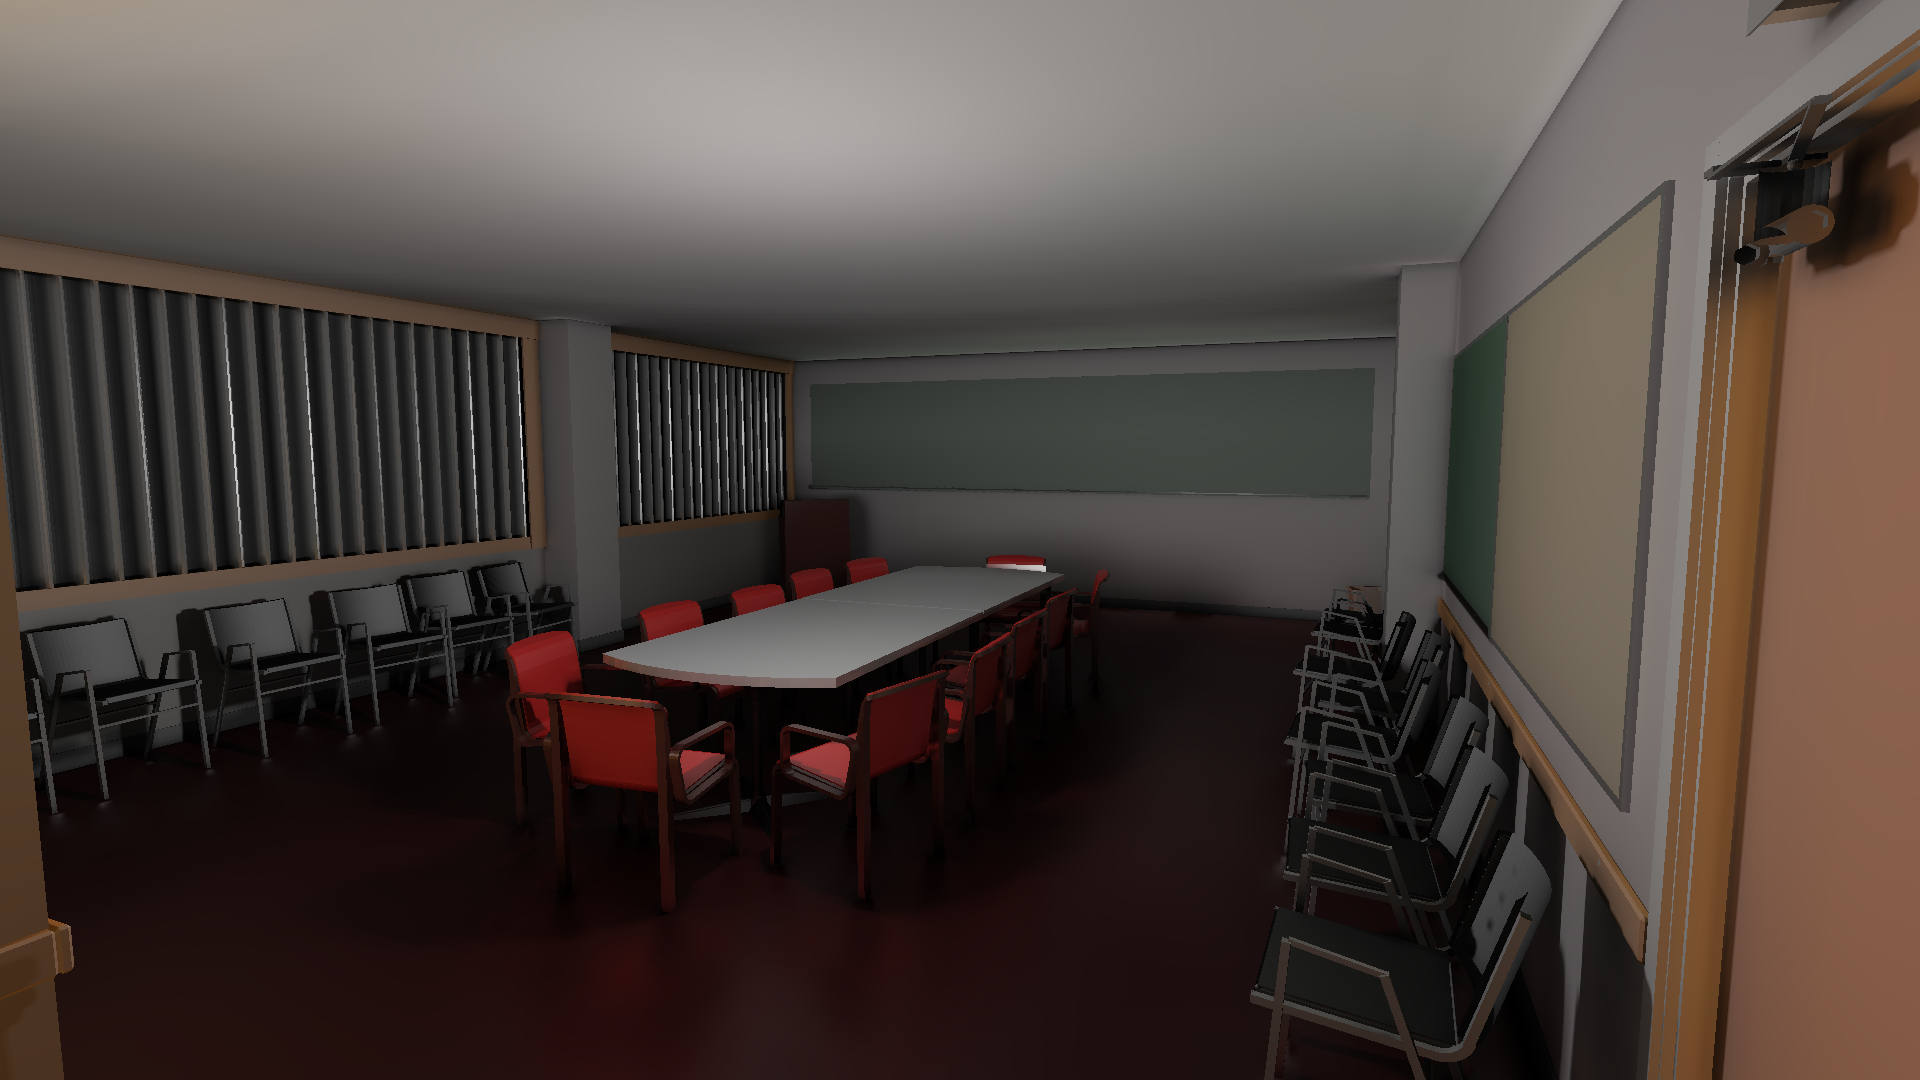
\includegraphics[width=\linewidth]{media/finals/conf_gi.png}
	\end{subfigure}%
	\caption{Composición para la escena Conference.}
	\label{fig:conf_final}
\end{figure}

\subsubsection{Iluminación Global de Vóxeles.}

En esta sección se demuestra la diferencia de imagen final al agregar iluminación global a la representación con vóxeles. La inclusión de iluminación global sobre los vóxeles nos permite aproximar el segundo rebote de luz. La diferencia entre imágenes fue procesada utilizando PerceptualDiff, los píxeles azules describen donde se encuentran las áreas con mayor diferencia al ojo humano.

\begin{figure}[H]
	\centering
	\begin{subfigure}[b]{.49\linewidth}
		\centering
		\captionsetup{justification=centering}
		\caption*{Directa, Indirecta y Oclusión Ambiental}
		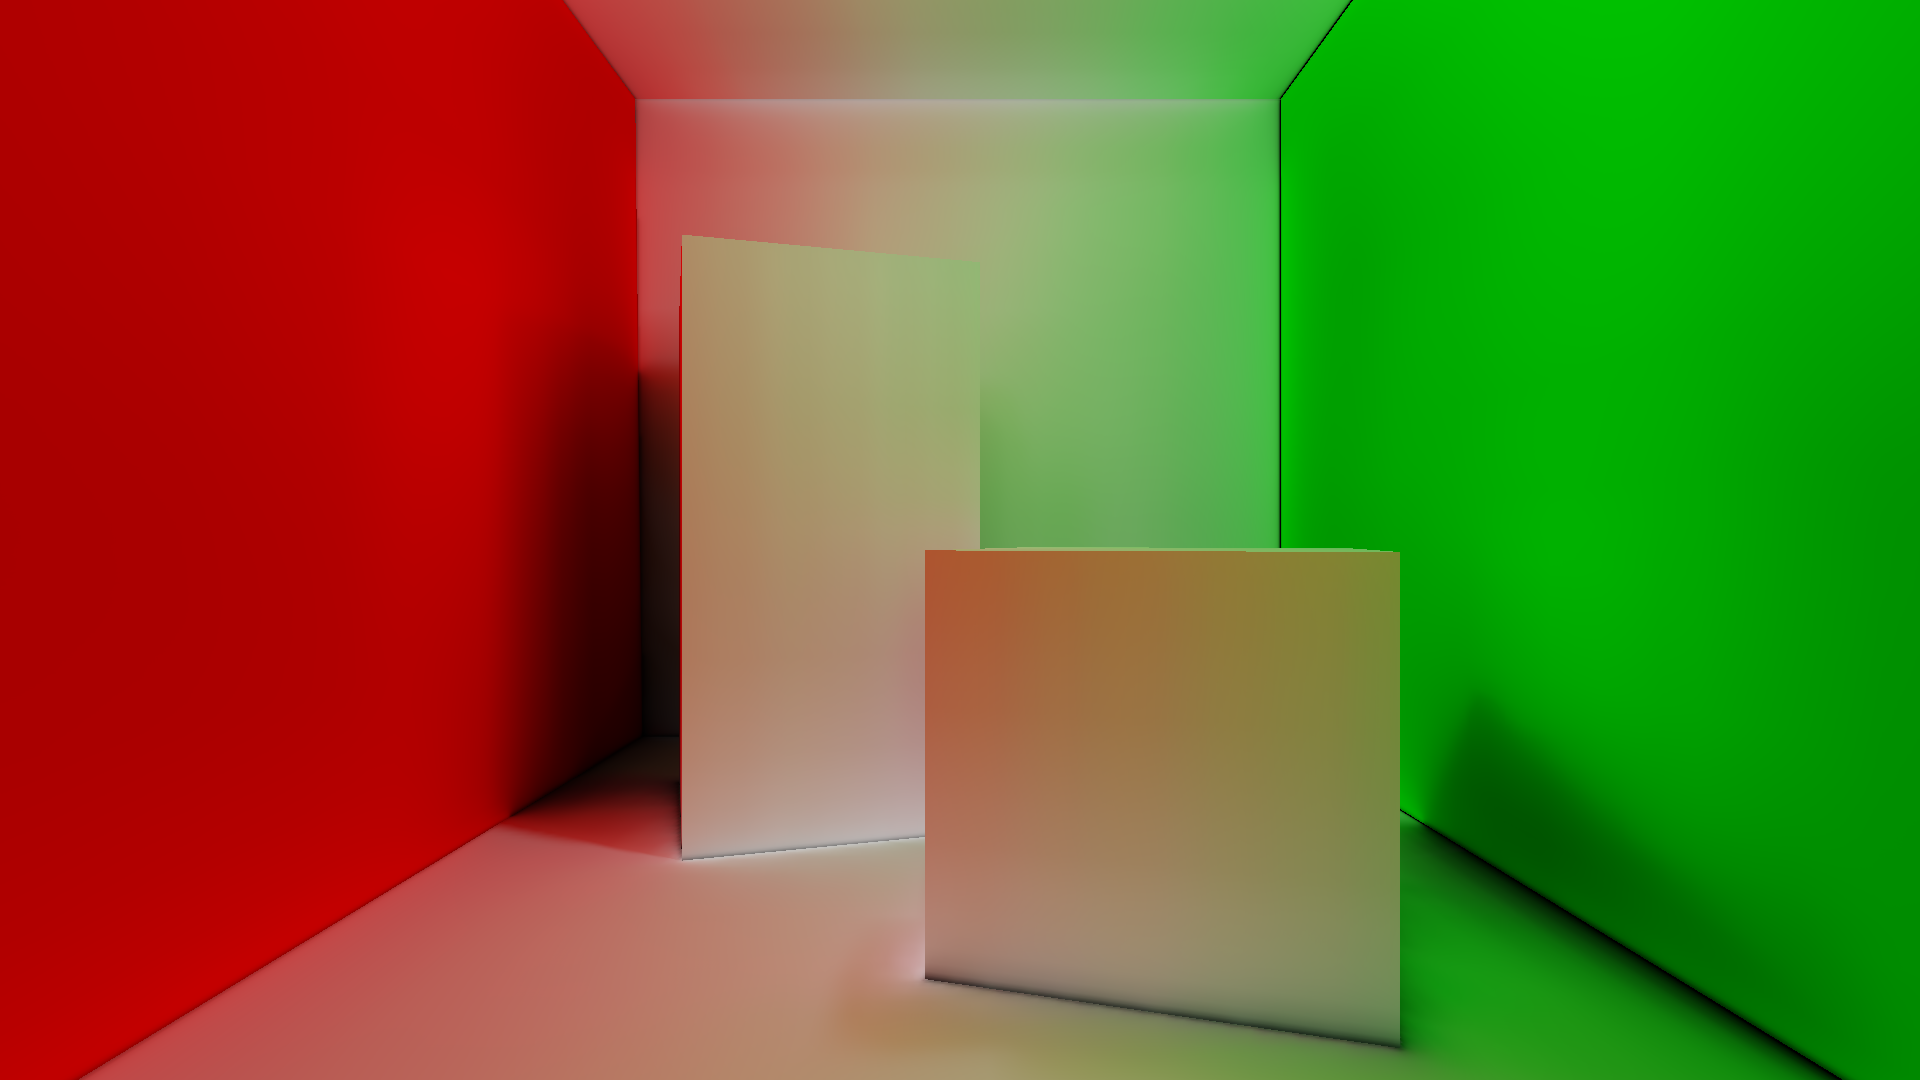
\includegraphics[width=\linewidth]{media/finals/cornell_vgi.png}
	\end{subfigure}%
	\hspace{0.01\textwidth}
	\begin{subfigure}[b]{.49\linewidth}
		\centering
		\captionsetup{justification=centering}
		\caption*{Diferencia Perceptual}
		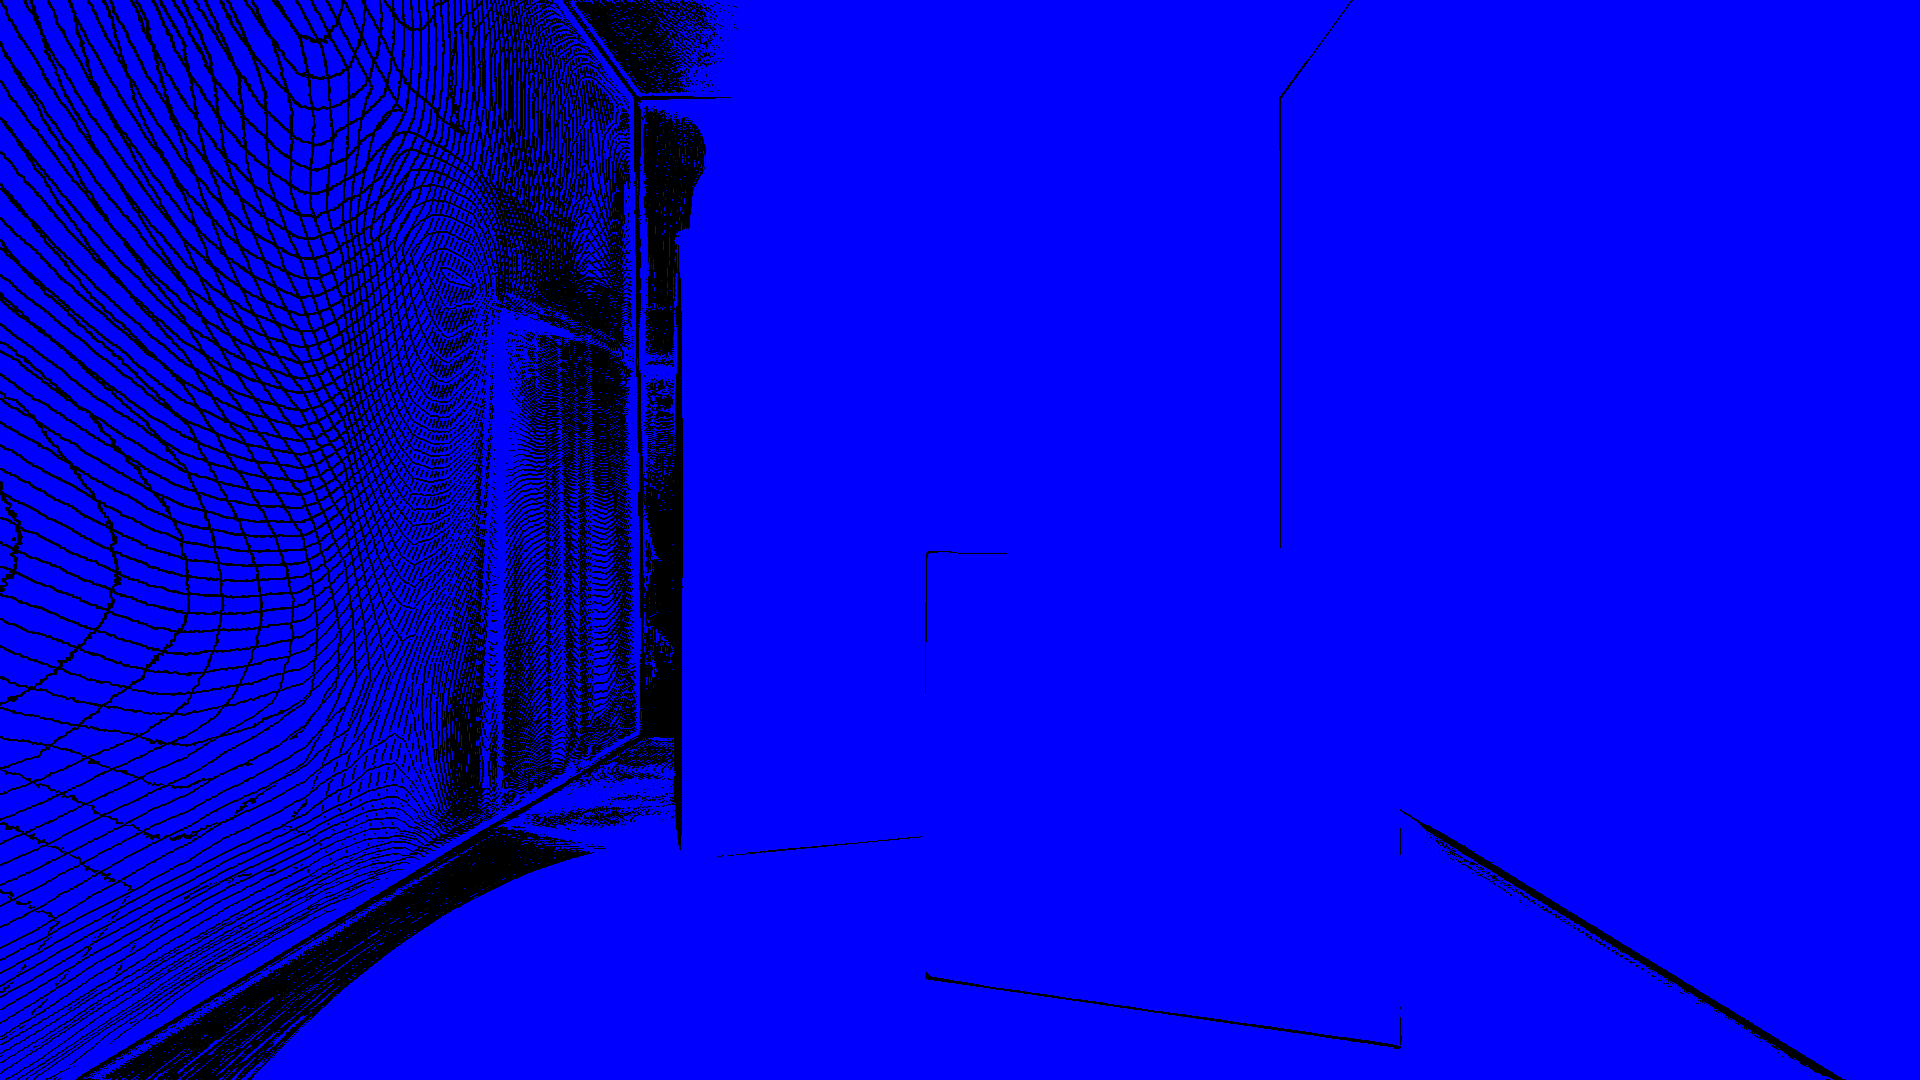
\includegraphics[width=\linewidth]{media/finals/cornell_vgi_diff.png}
	\end{subfigure}%
	\caption{Diferencia perceptual con respecto a la imagen \ref{fig:cornell_final} al habilitar iluminación global de vóxeles.}
	\label{fig:cornell_vgi_diff}
\end{figure}
\begin{figure}[H]
	\centering
	\begin{subfigure}[b]{.49\linewidth}
		\centering
		\captionsetup{justification=centering}
		%\caption*{Sombreado e Iluminación Global de Vóxeles}
		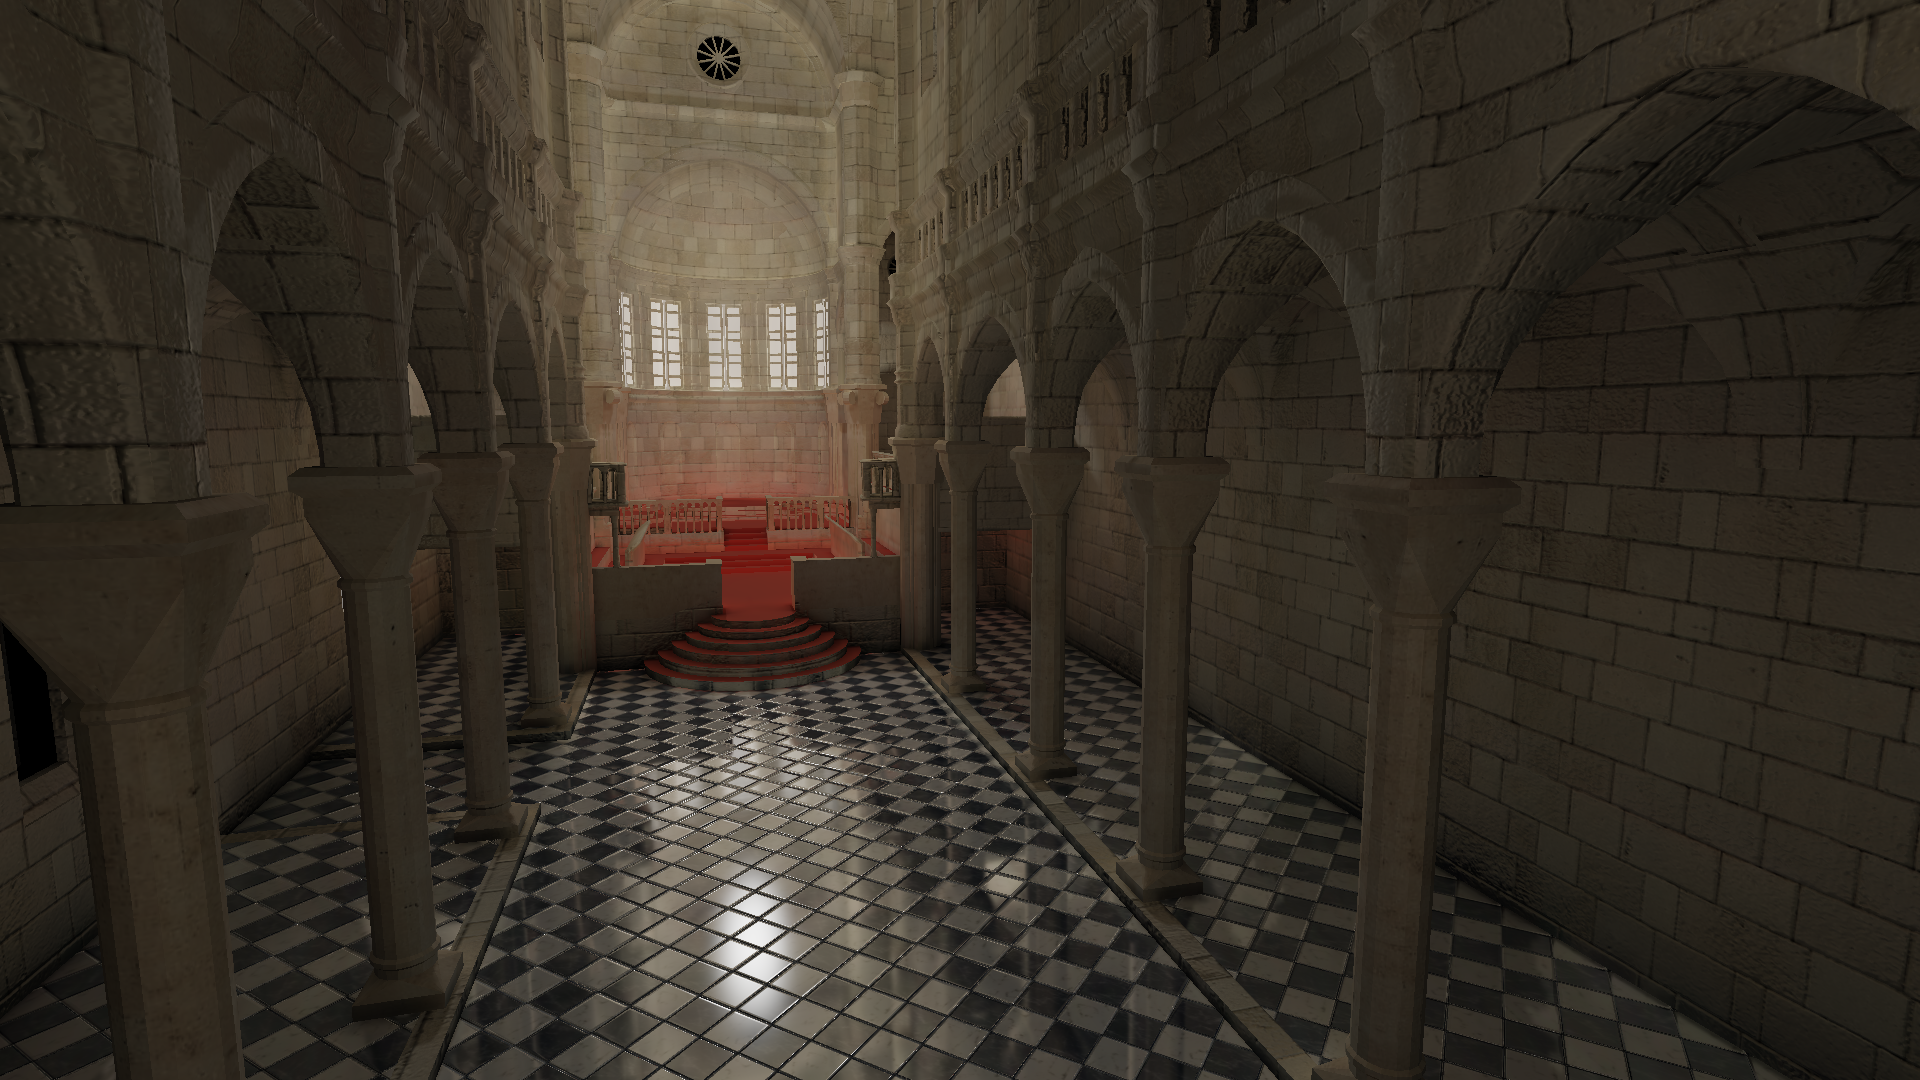
\includegraphics[width=\linewidth]{media/finals/sibenik_vgi.png}
	\end{subfigure}%
	\hspace{0.01\textwidth}
	\begin{subfigure}[b]{.49\linewidth}
		\centering
		\captionsetup{justification=centering}
		%\caption*{Diferencia Perceptual}
		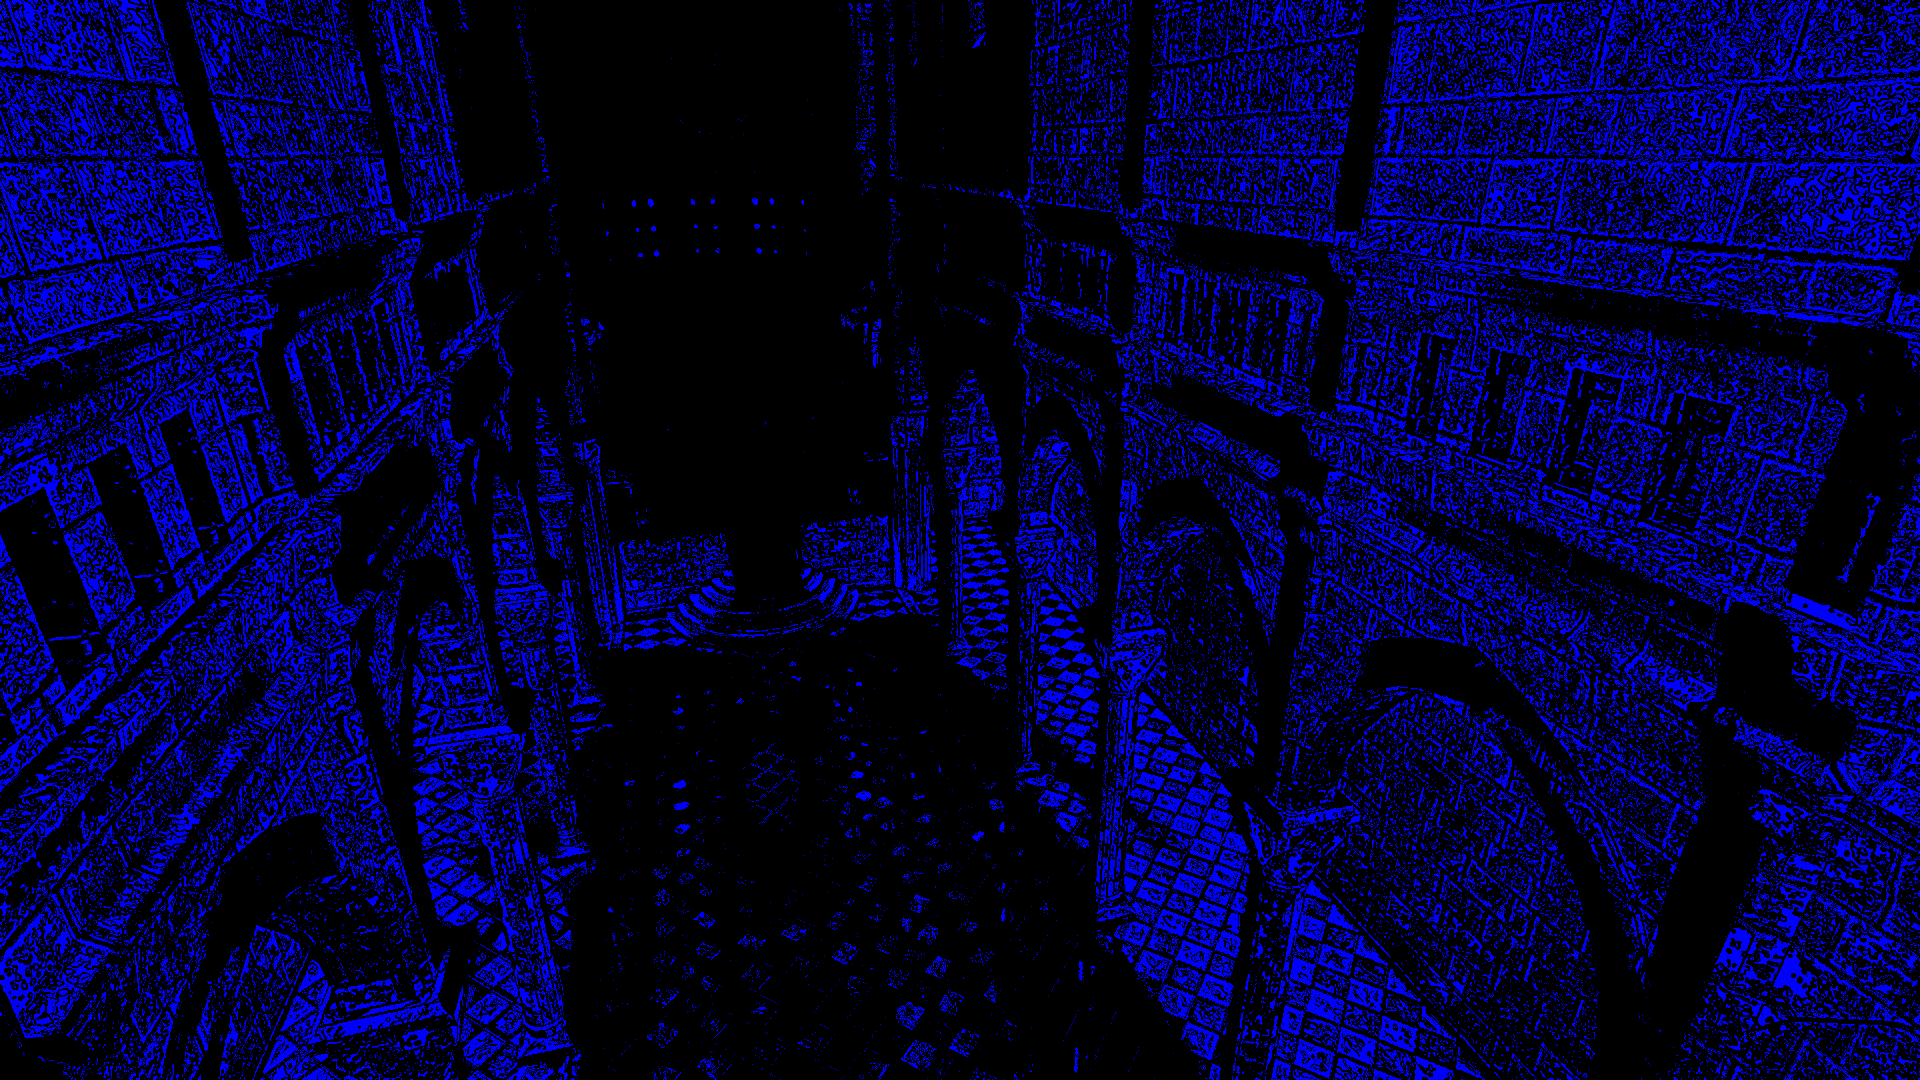
\includegraphics[width=\linewidth]{media/finals/sibenik_vgi_diff.png}
	\end{subfigure}%
	\caption{Diferencia perceptual con respecto a la imagen \ref{fig:sibenik_final} al habilitar iluminación global de vóxeles.}
	\label{fig:sibenik_vgi_diff}
\end{figure}
\begin{figure}[H]
	\centering
	\begin{subfigure}[b]{.49\linewidth}
		\centering
		\captionsetup{justification=centering}
		%\caption*{Sombreado e Iluminación Global de Vóxeles}
		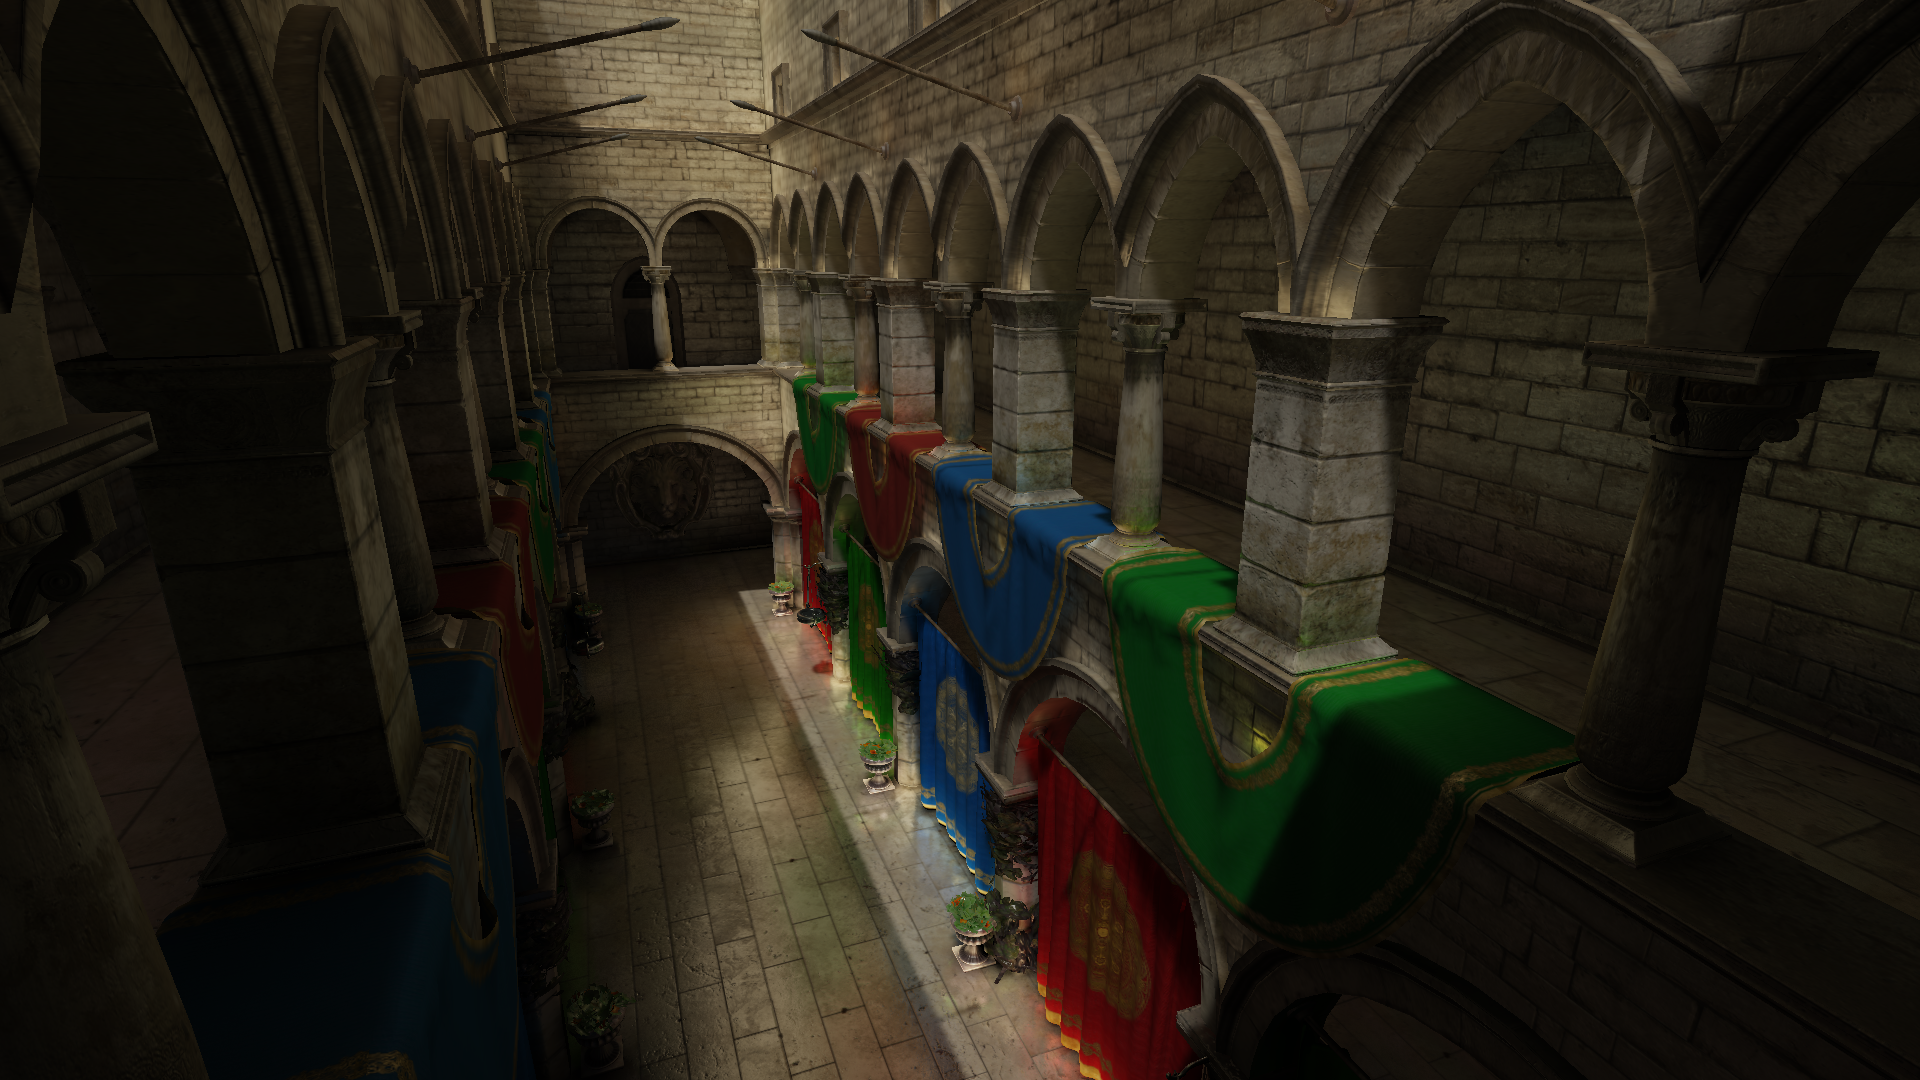
\includegraphics[width=\linewidth]{media/finals/sponza_vgi.png}
	\end{subfigure}%
	\hspace{0.01\textwidth}
	\begin{subfigure}[b]{.49\linewidth}
		\centering
		\captionsetup{justification=centering}
		%\caption*{Diferencia Perceptual}
		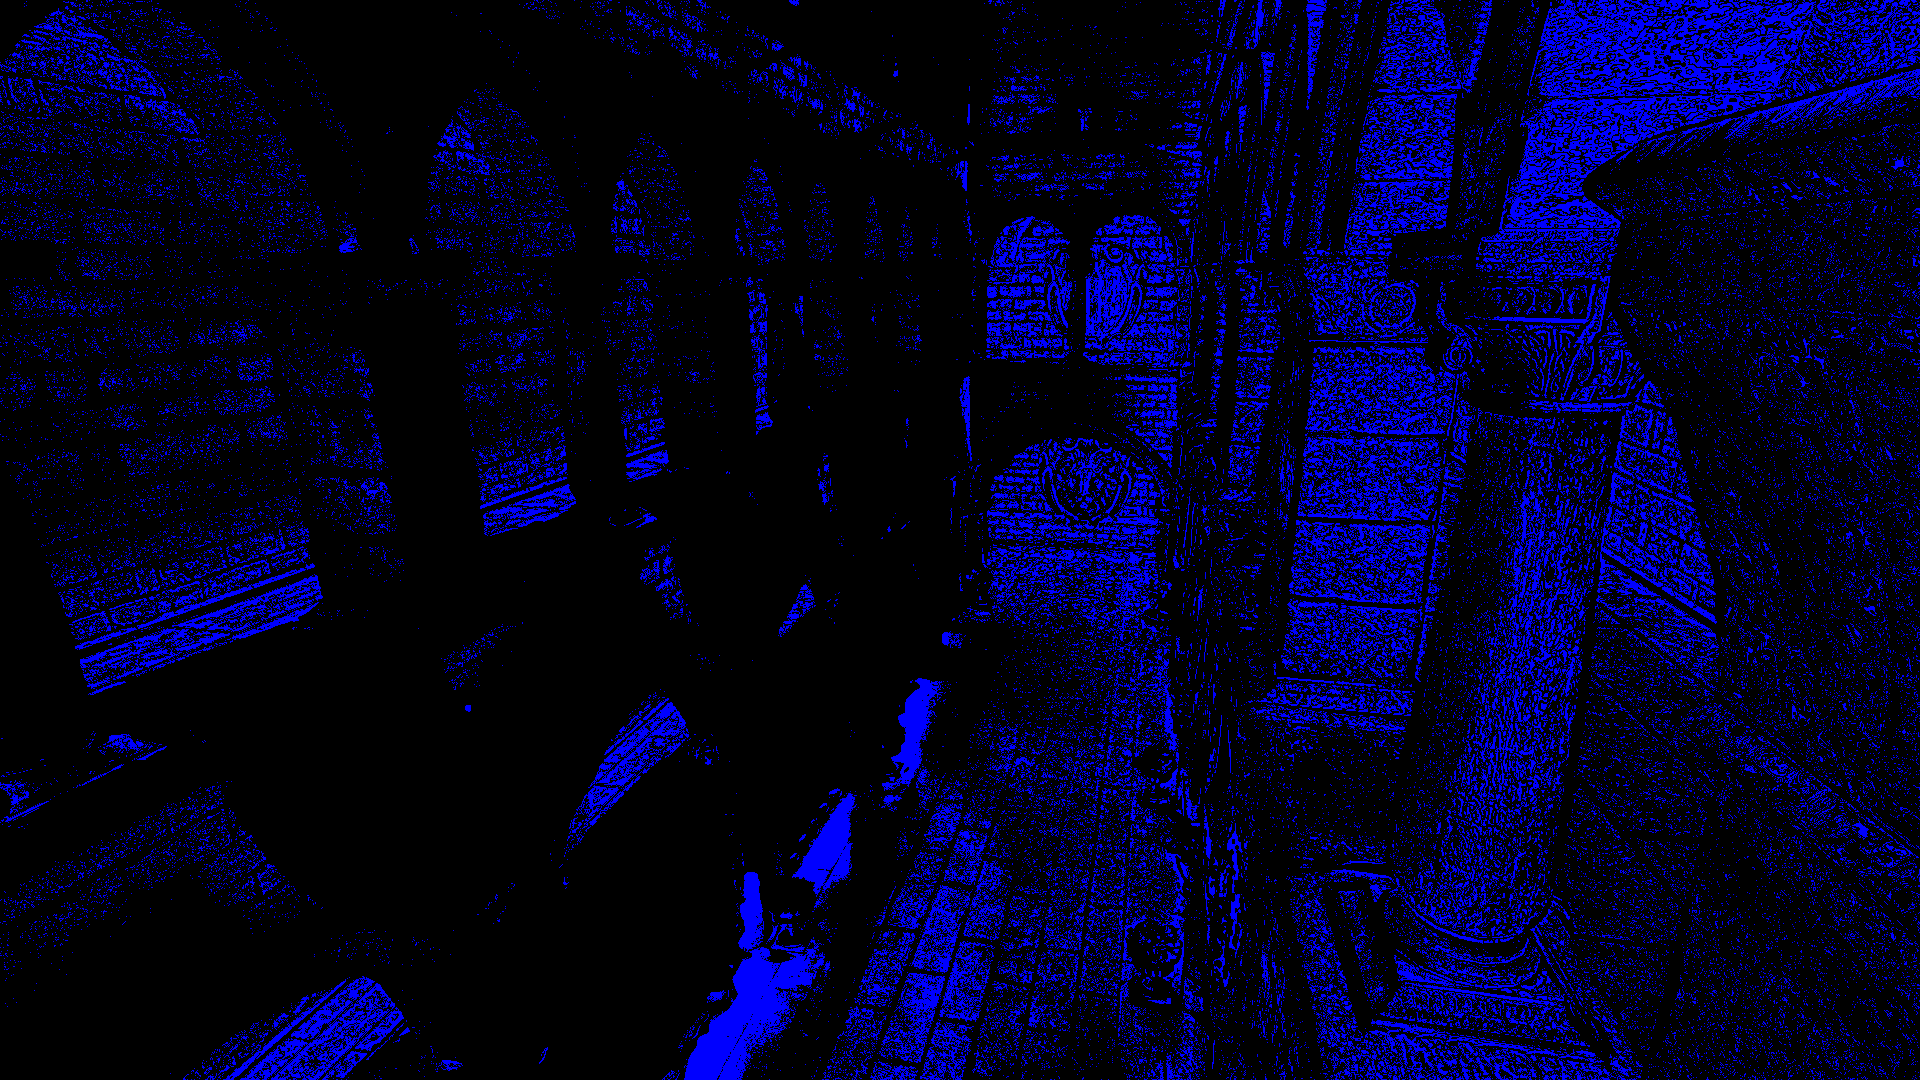
\includegraphics[width=\linewidth]{media/finals/sponza_vgi_diff.png}
	\end{subfigure}%
	\caption{Diferencia perceptual con respecto a la imagen \ref{fig:sponza_final} al habilitar iluminación global de vóxeles.}
	\label{fig:sponza_vgi_diff}
\end{figure}
\begin{figure}[H]
	\centering
	\begin{subfigure}[b]{.49\linewidth}
		\centering
		\captionsetup{justification=centering}
		%\caption*{Sombreado e Iluminación Global de Vóxeles}
		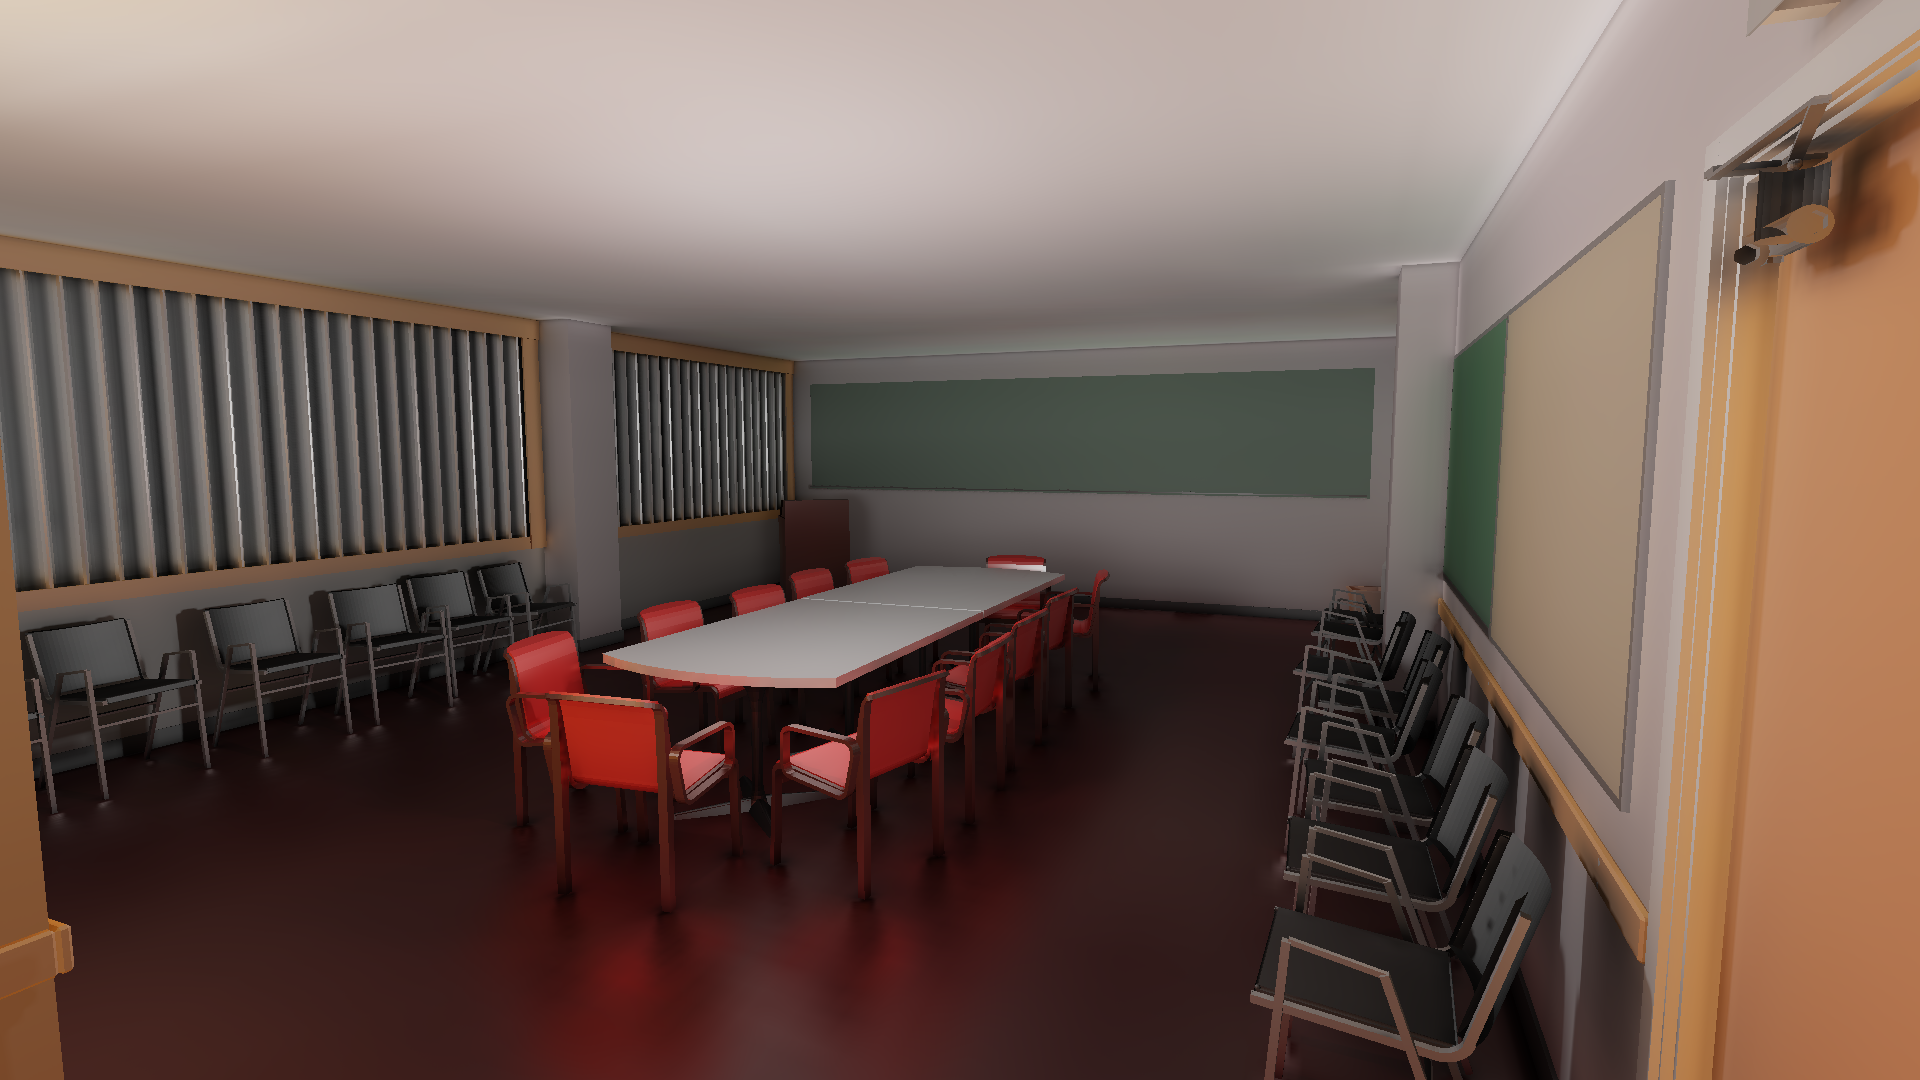
\includegraphics[width=\linewidth]{media/finals/conf_vgi.png}
	\end{subfigure}%
	\hspace{0.01\textwidth}
	\begin{subfigure}[b]{.49\linewidth}
		\centering
		\captionsetup{justification=centering}
		%\caption*{Diferencia Perceptual}
		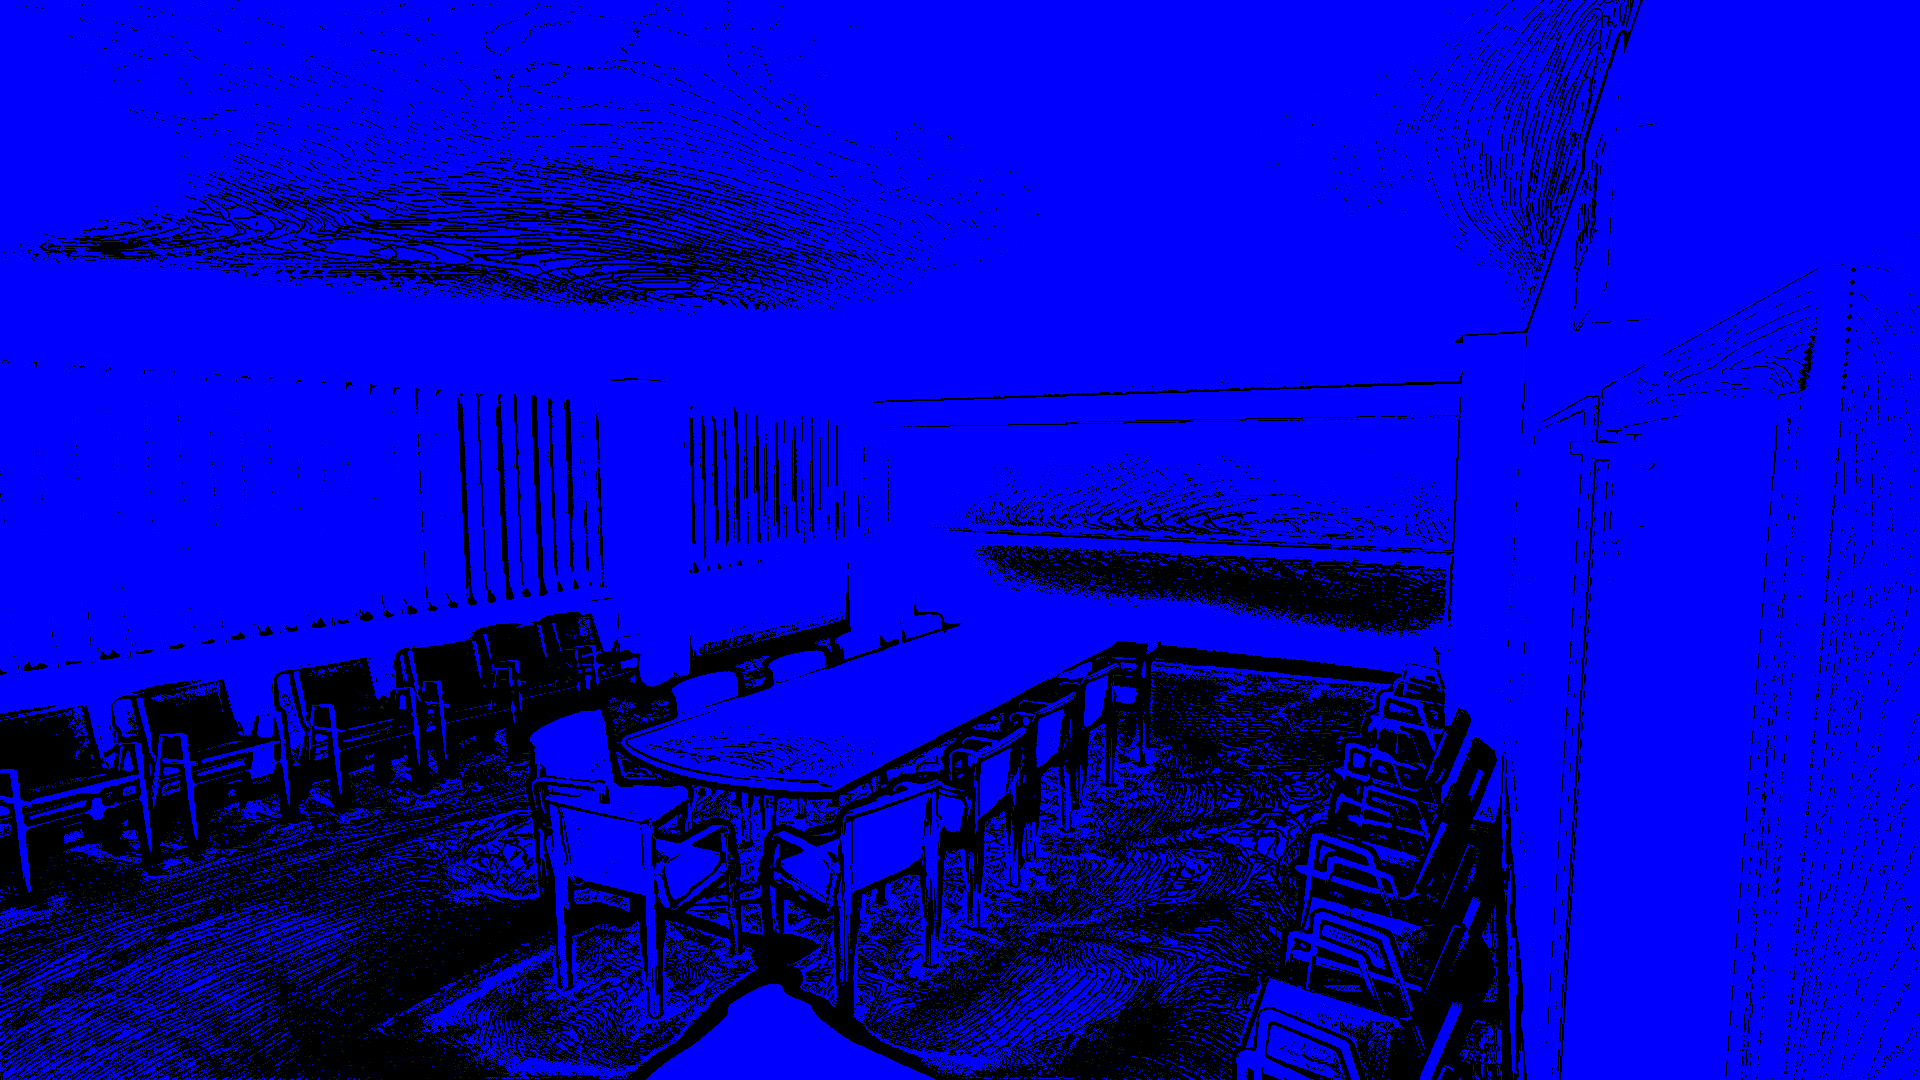
\includegraphics[width=\linewidth]{media/finals/conf_vgi_diff.png}
	\end{subfigure}%
	\caption{Diferencia perceptual con respecto a la imagen \ref{fig:conf_final} al habilitar iluminación global de vóxeles.}
	\label{fig:conf_vgi_diff}
\end{figure}

\subsubsection{Resolución de la Representación en Vóxeles}

En esta sección se demuestra la diferencia de imagen final con distintas resoluciones para la representación en vóxeles. Todas las imágenes serán comparadas con los resultados de la sección \ref{subsec:final} donde se utiliza una resolución para los volúmenes de $512^3$ sin iluminación global de vóxeles. En las imágenes se puede apreciar como la diferencia aumenta a medida que se disminuye la resolución.

\begin{figure}[H]
	\centering
	\begin{subfigure}[b]{.49\linewidth}
		\centering
		\captionsetup{justification=centering}
		\caption*{Directa, Indirecta y Oclusión Ambiental}
		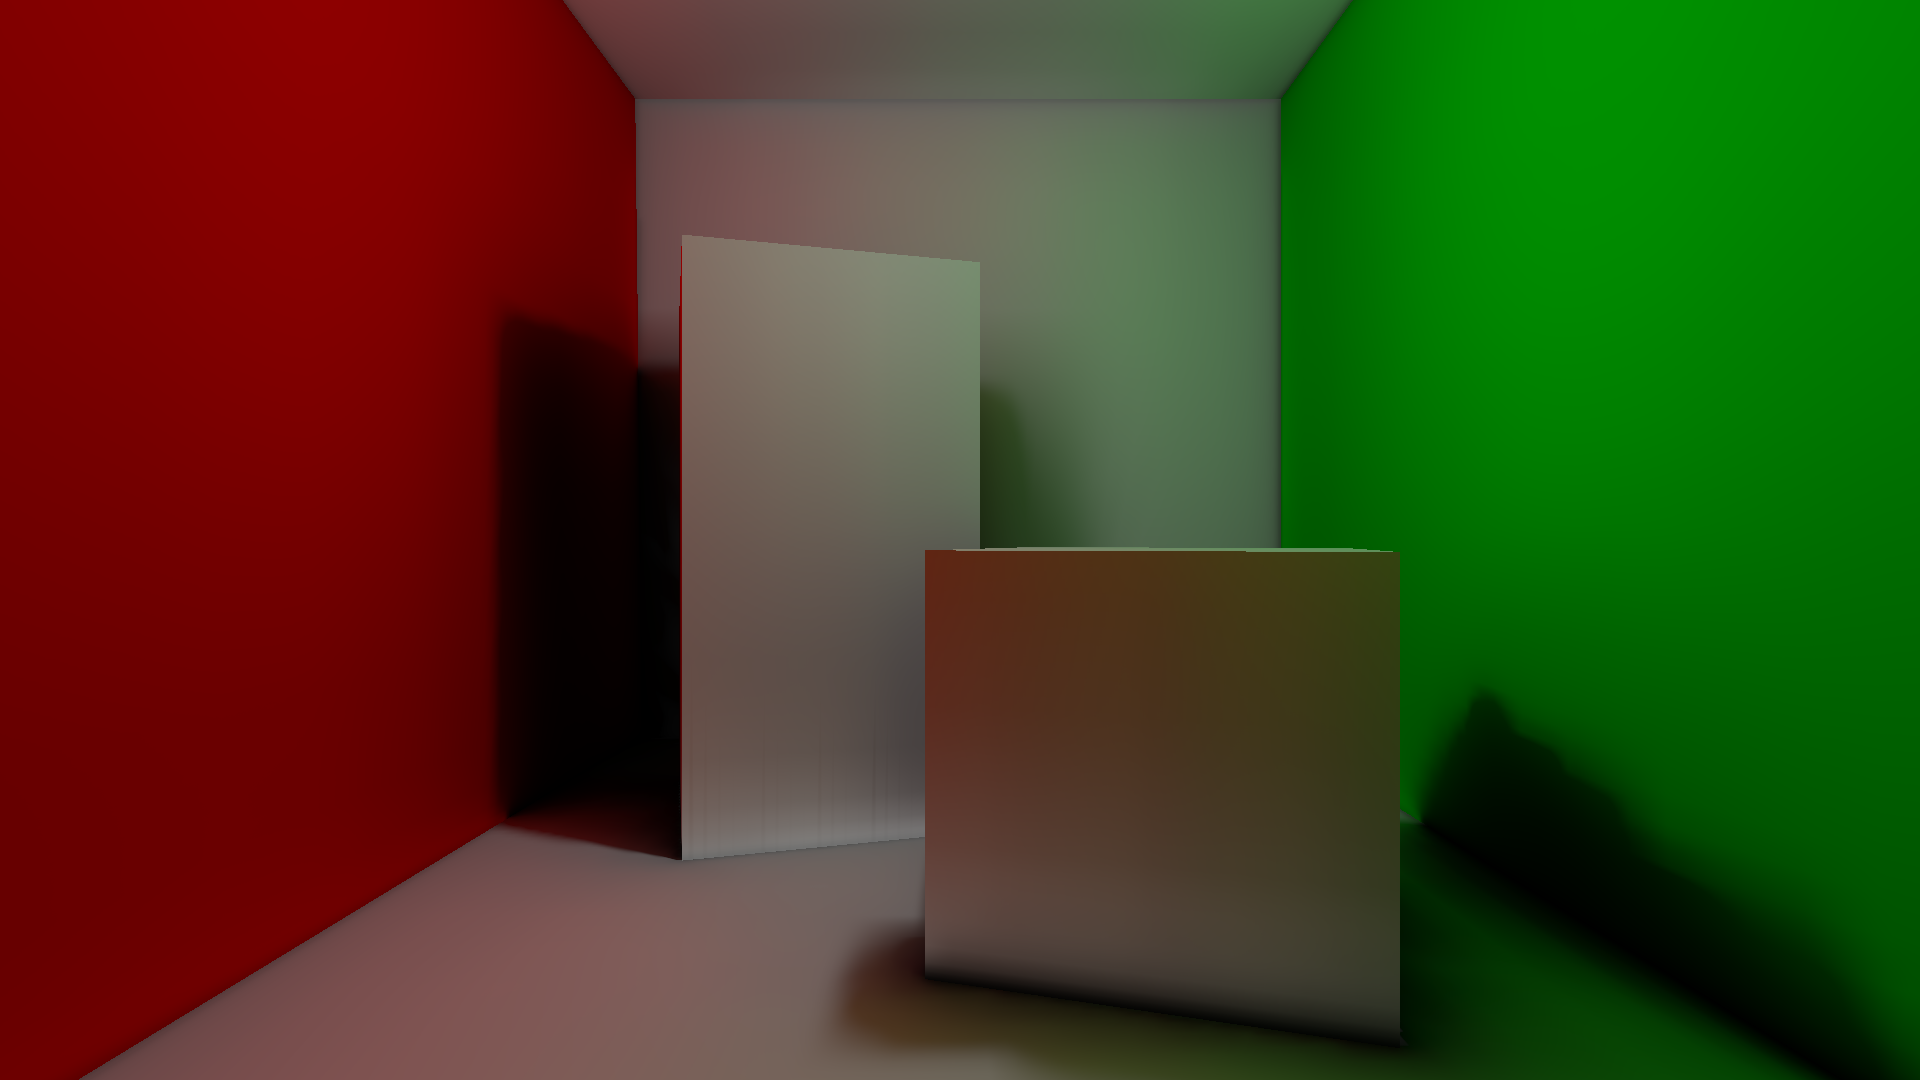
\includegraphics[width=\linewidth]{media/finals/cornell_gi_256.png}
		\caption*{$256^3$}
	\end{subfigure}%
	\hspace{0.01\textwidth}
	\begin{subfigure}[b]{.49\linewidth}
		\centering
		\captionsetup{justification=centering}
		\caption*{Diferencia Perceptual\\}
		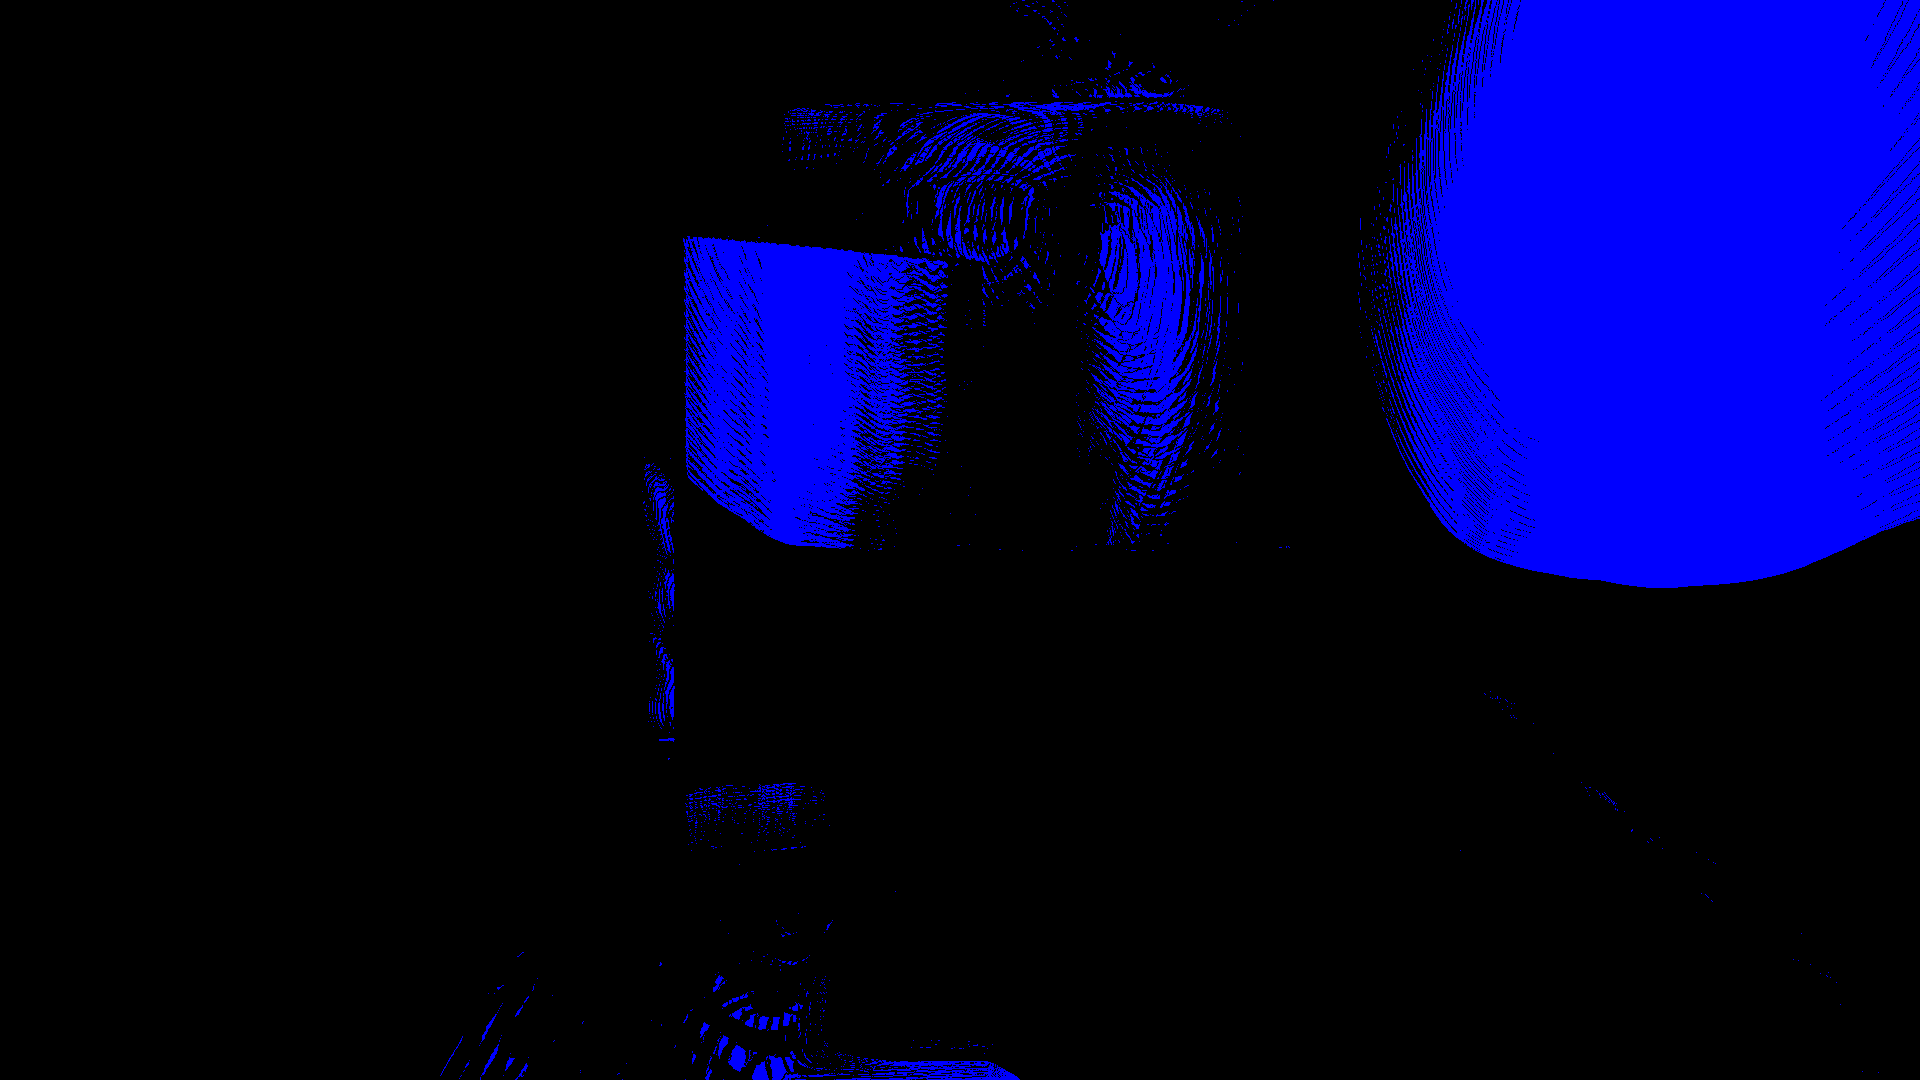
\includegraphics[width=\linewidth]{media/finals/cornell_gi_256_diff.png}
		\caption*{}
	\end{subfigure}%
	\par\smallskip
	\begin{subfigure}[b]{.49\linewidth}
		\centering
		\captionsetup{justification=centering}
		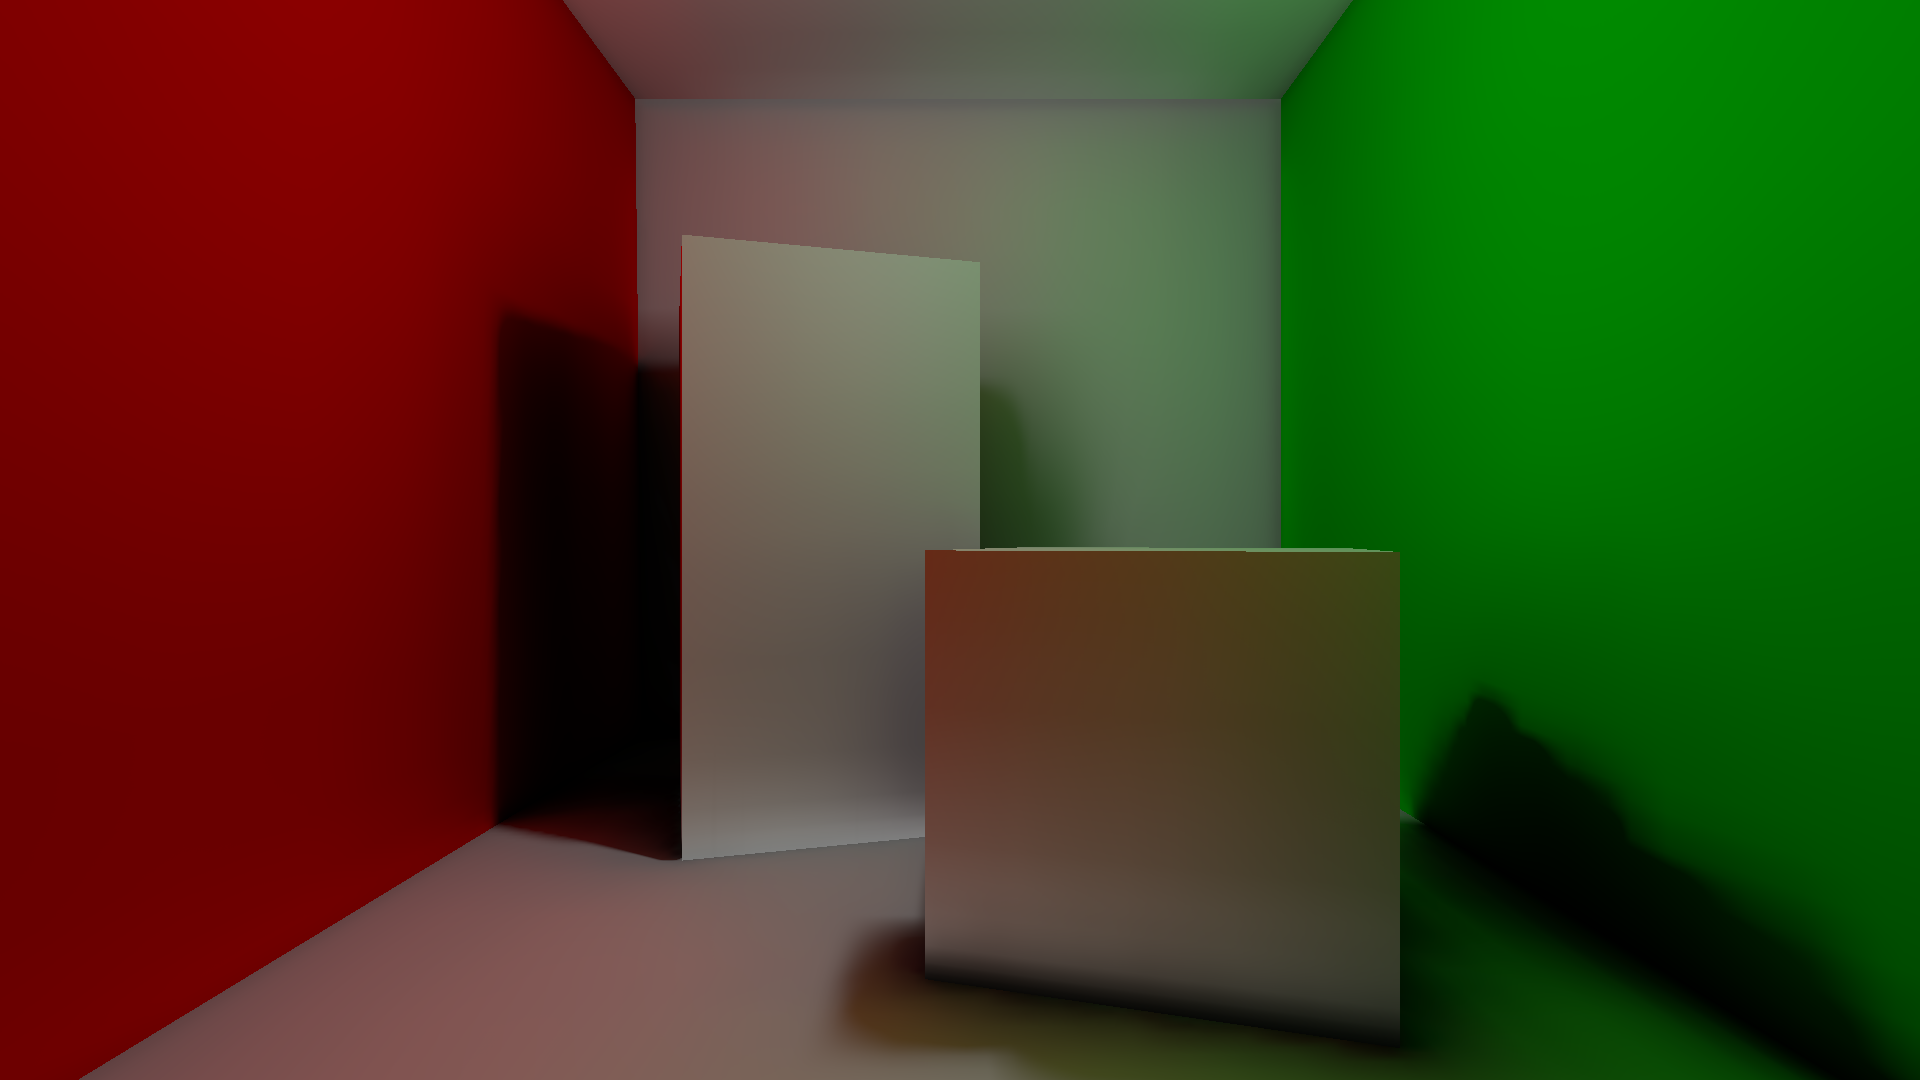
\includegraphics[width=\linewidth]{media/finals/cornell_gi_128.png}
		\caption*{$128^3$}
	\end{subfigure}%
	\hspace{0.01\textwidth}
	\begin{subfigure}[b]{.49\linewidth}
		\centering
		\captionsetup{justification=centering}
		%\caption*{Diferencia Perceptual}
		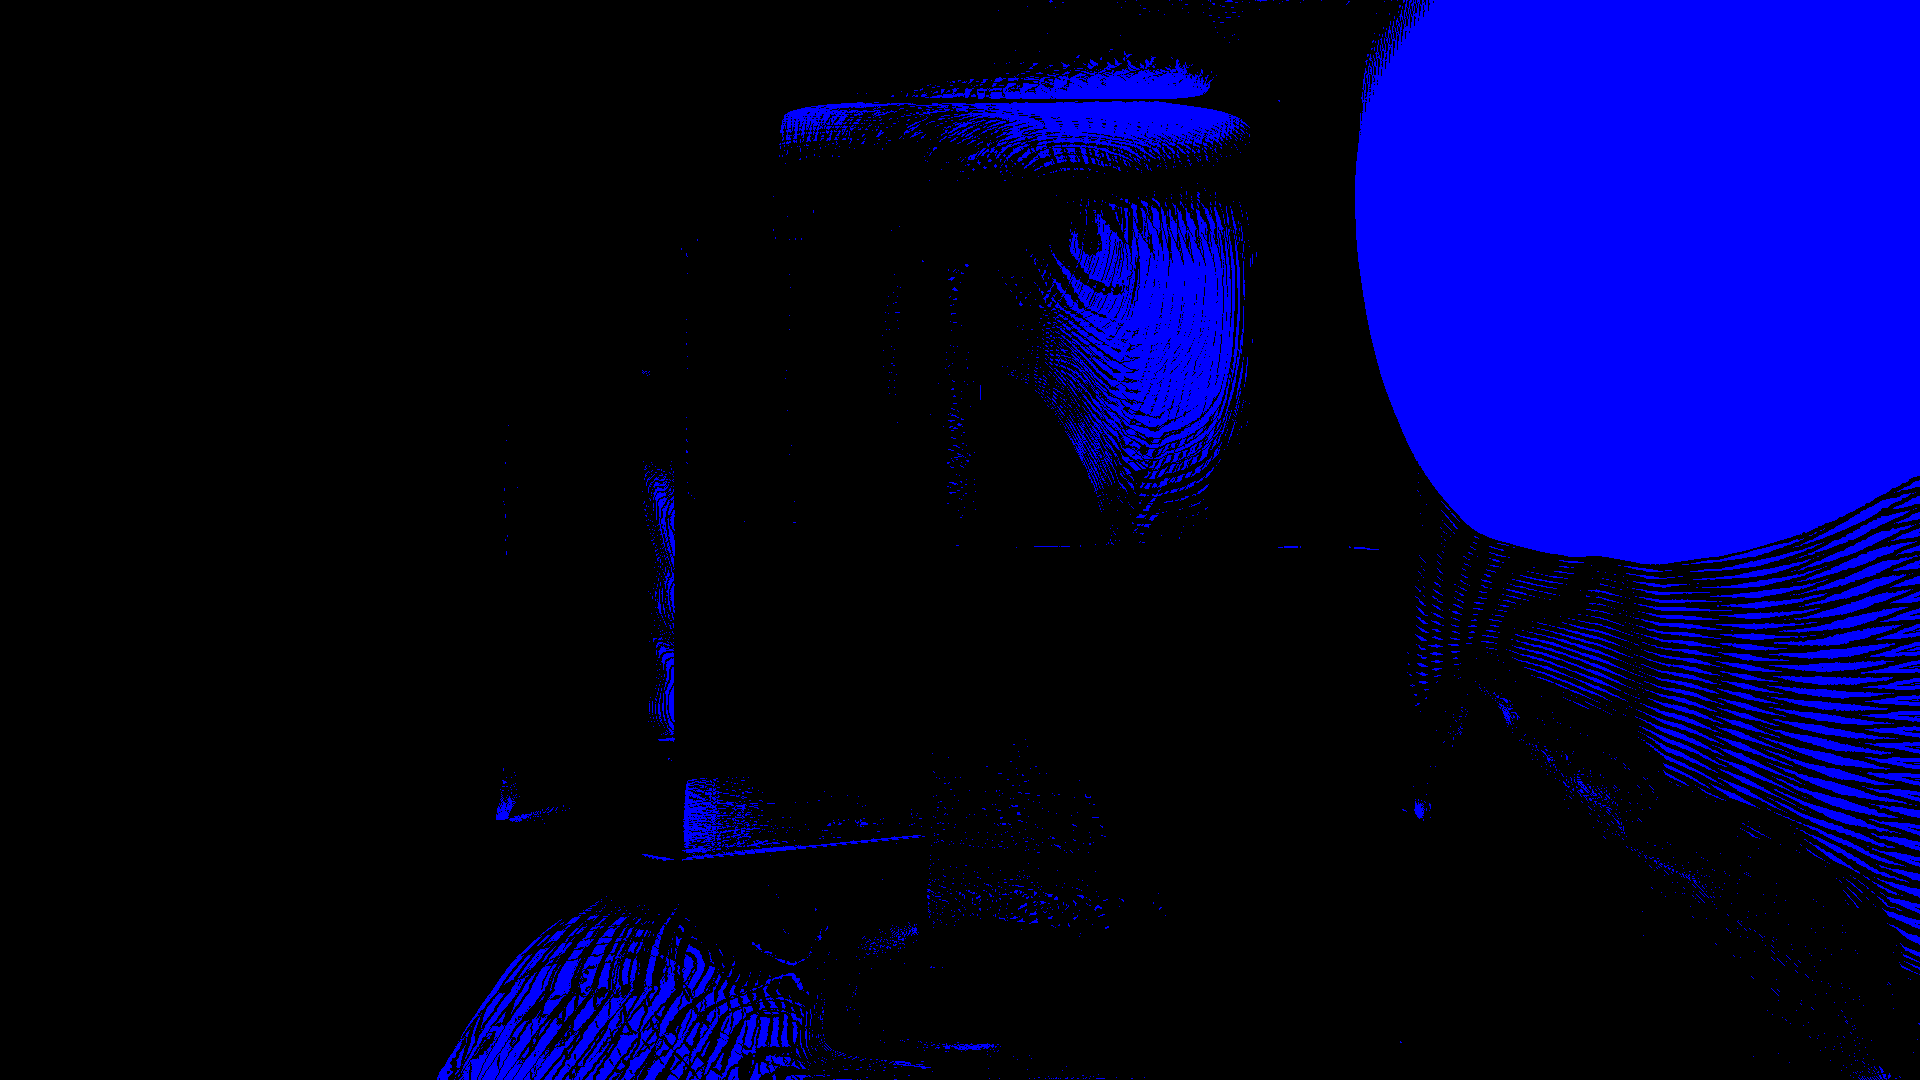
\includegraphics[width=\linewidth]{media/finals/cornell_gi_128_diff.png}
		\caption*{}
	\end{subfigure}%
	\par\smallskip
	\begin{subfigure}[b]{.49\linewidth}
		\centering
		\captionsetup{justification=centering}
		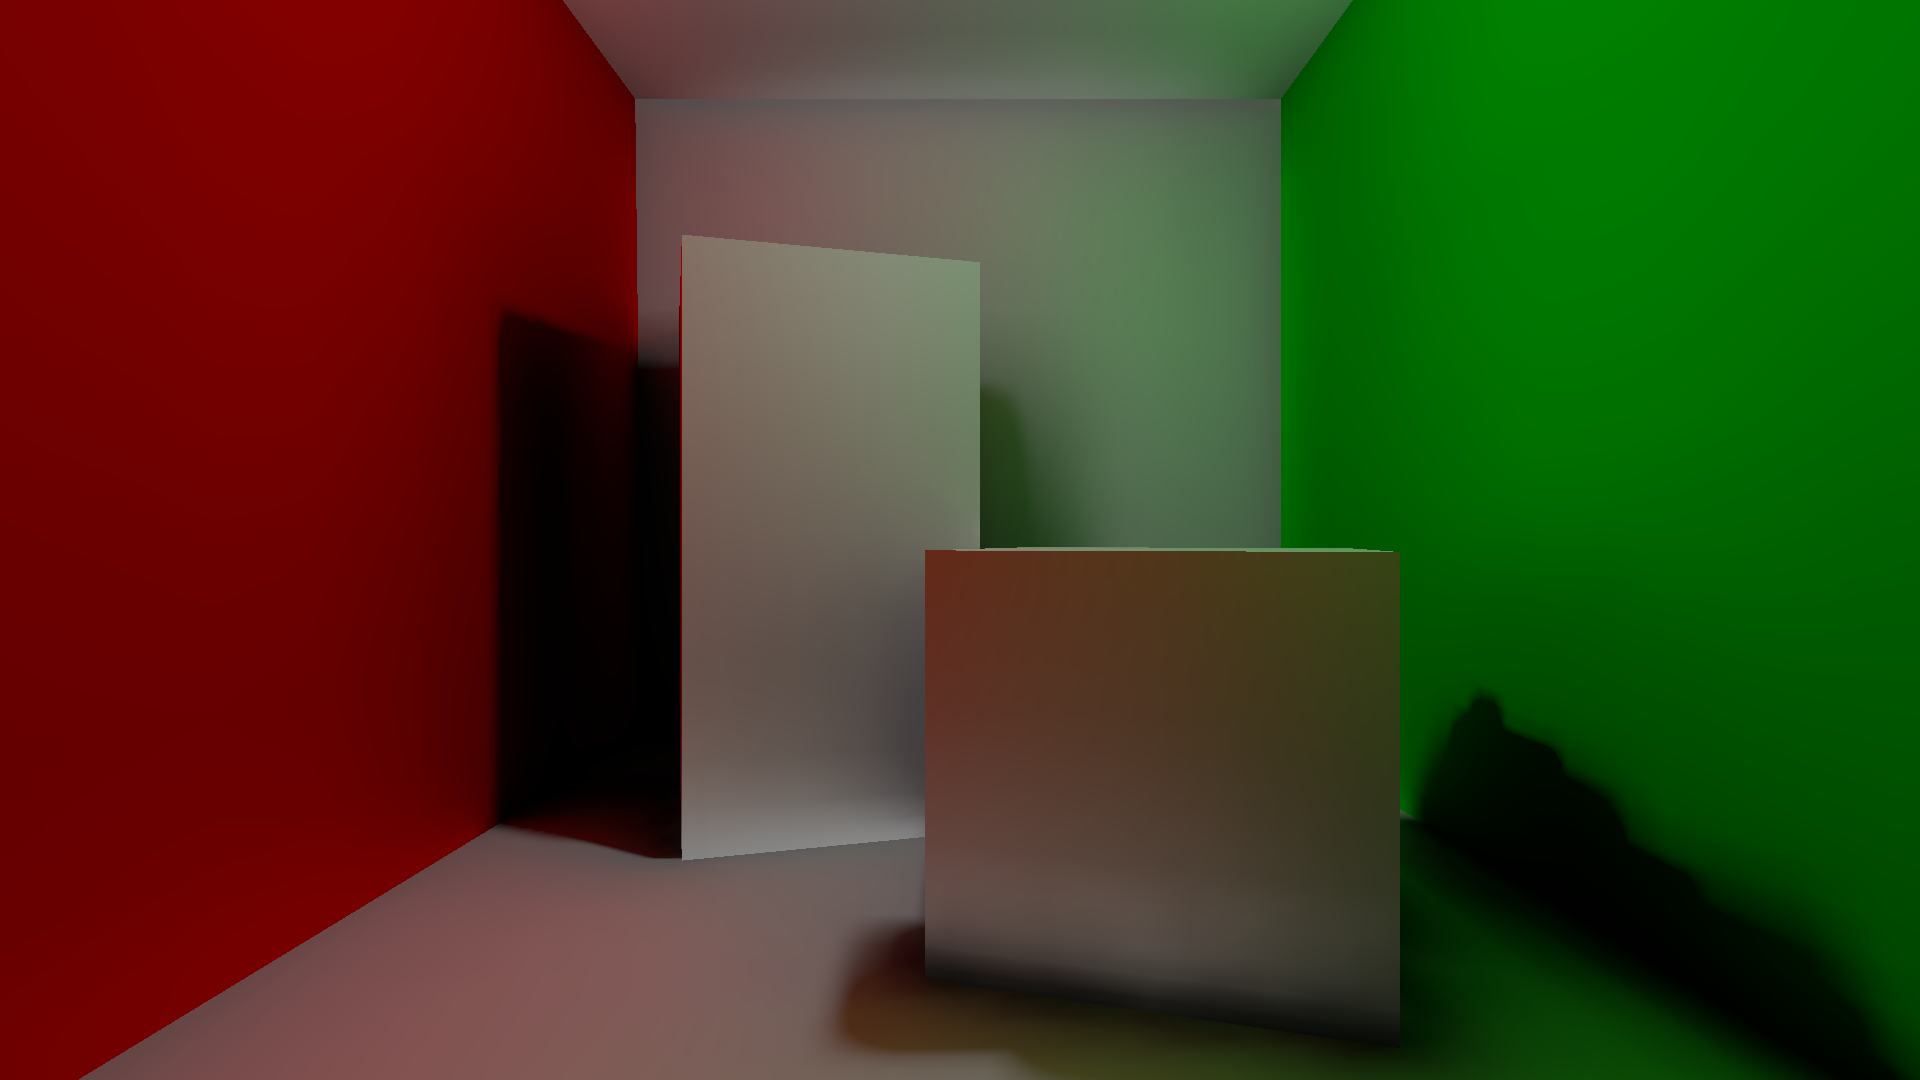
\includegraphics[width=\linewidth]{media/finals/cornell_gi_64.png}
		\caption*{$64^3$}
	\end{subfigure}%
	\hspace{0.01\textwidth}
	\begin{subfigure}[b]{.49\linewidth}
		\centering
		\captionsetup{justification=centering}
		%\caption*{Diferencia Perceptual}
		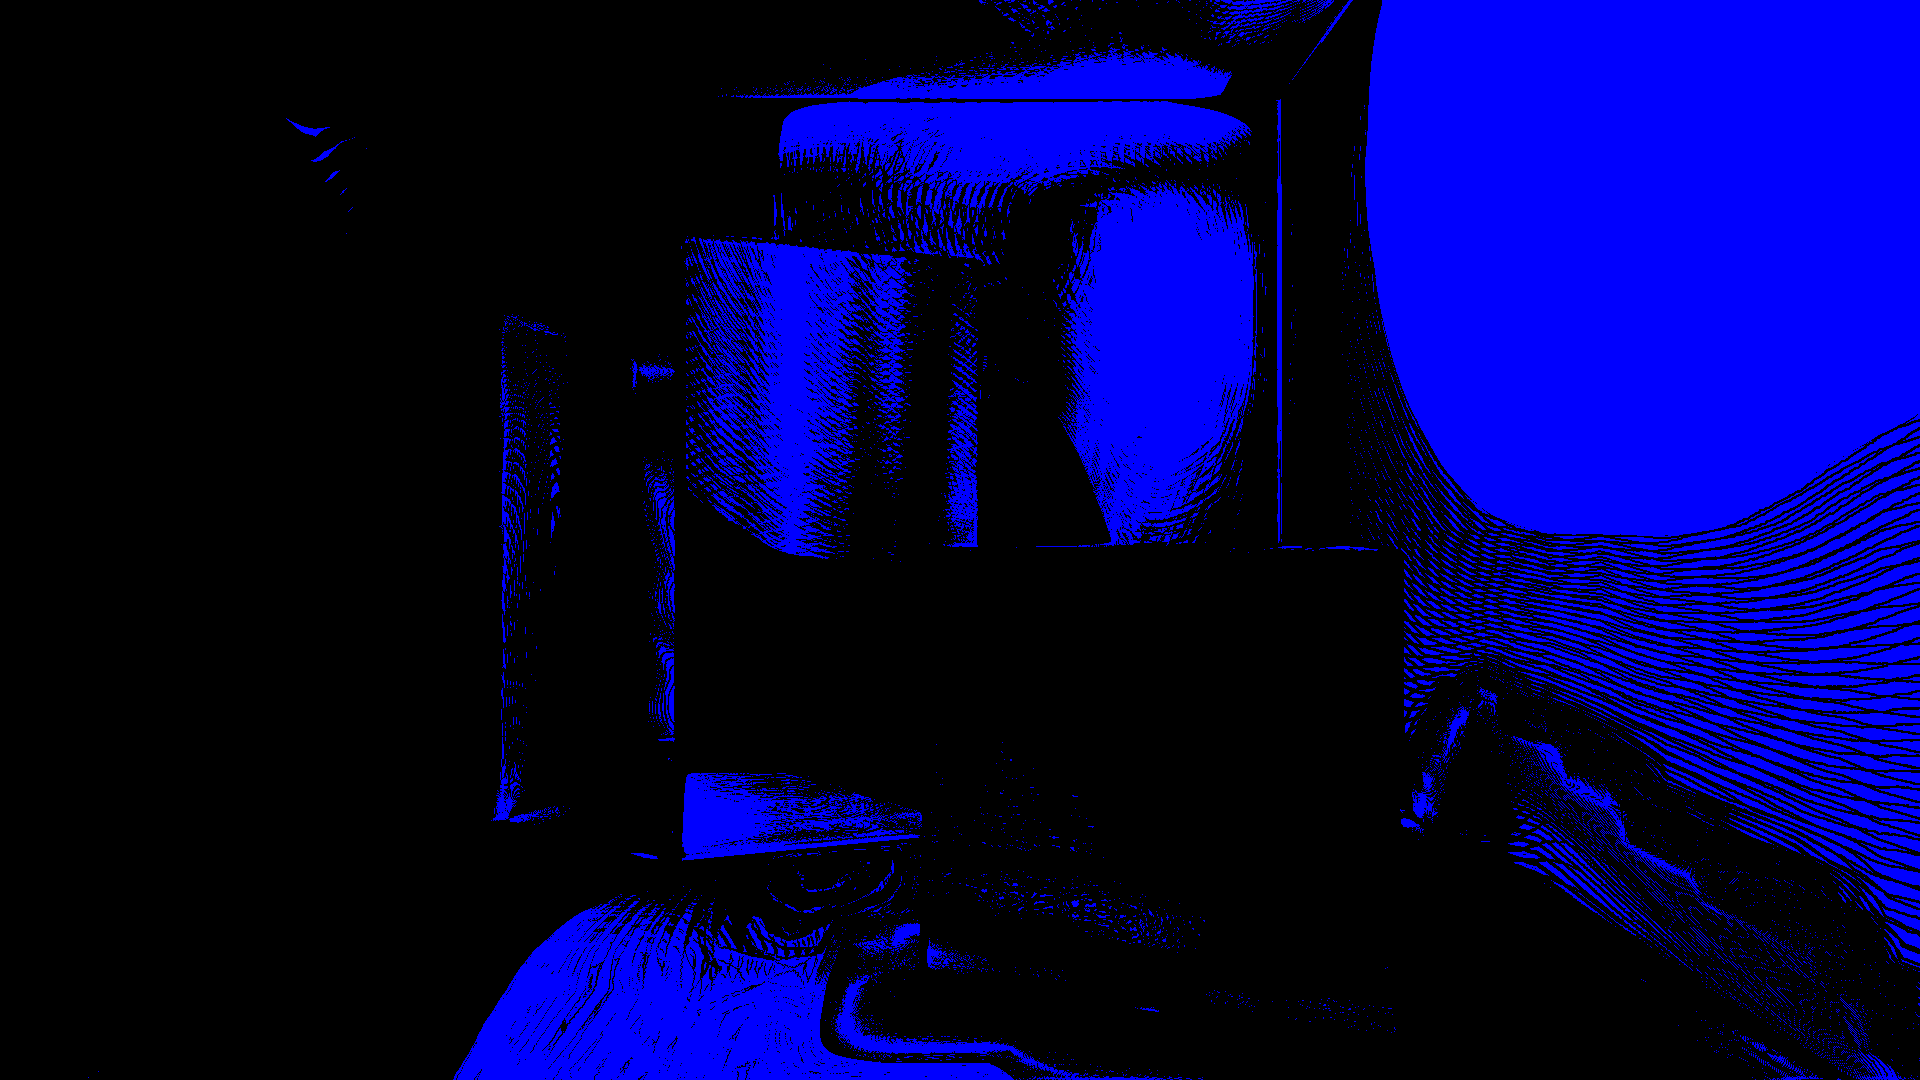
\includegraphics[width=\linewidth]{media/finals/cornell_gi_64_diff.png}
		\caption*{}
	\end{subfigure}%
	\caption{Diferencia visual con respecto a la imagen \ref{fig:cornell_final} utilizando distintas resoluciones para la representación en vóxeles.}
	\label{fig:cornell_gi_resdiff}
\end{figure}

\begin{figure}[H]
	\centering
	\begin{subfigure}[b]{.49\linewidth}
		\centering
		\captionsetup{justification=centering}
		%\caption*{Directa, Indirecta y Oclusión Ambiental}
		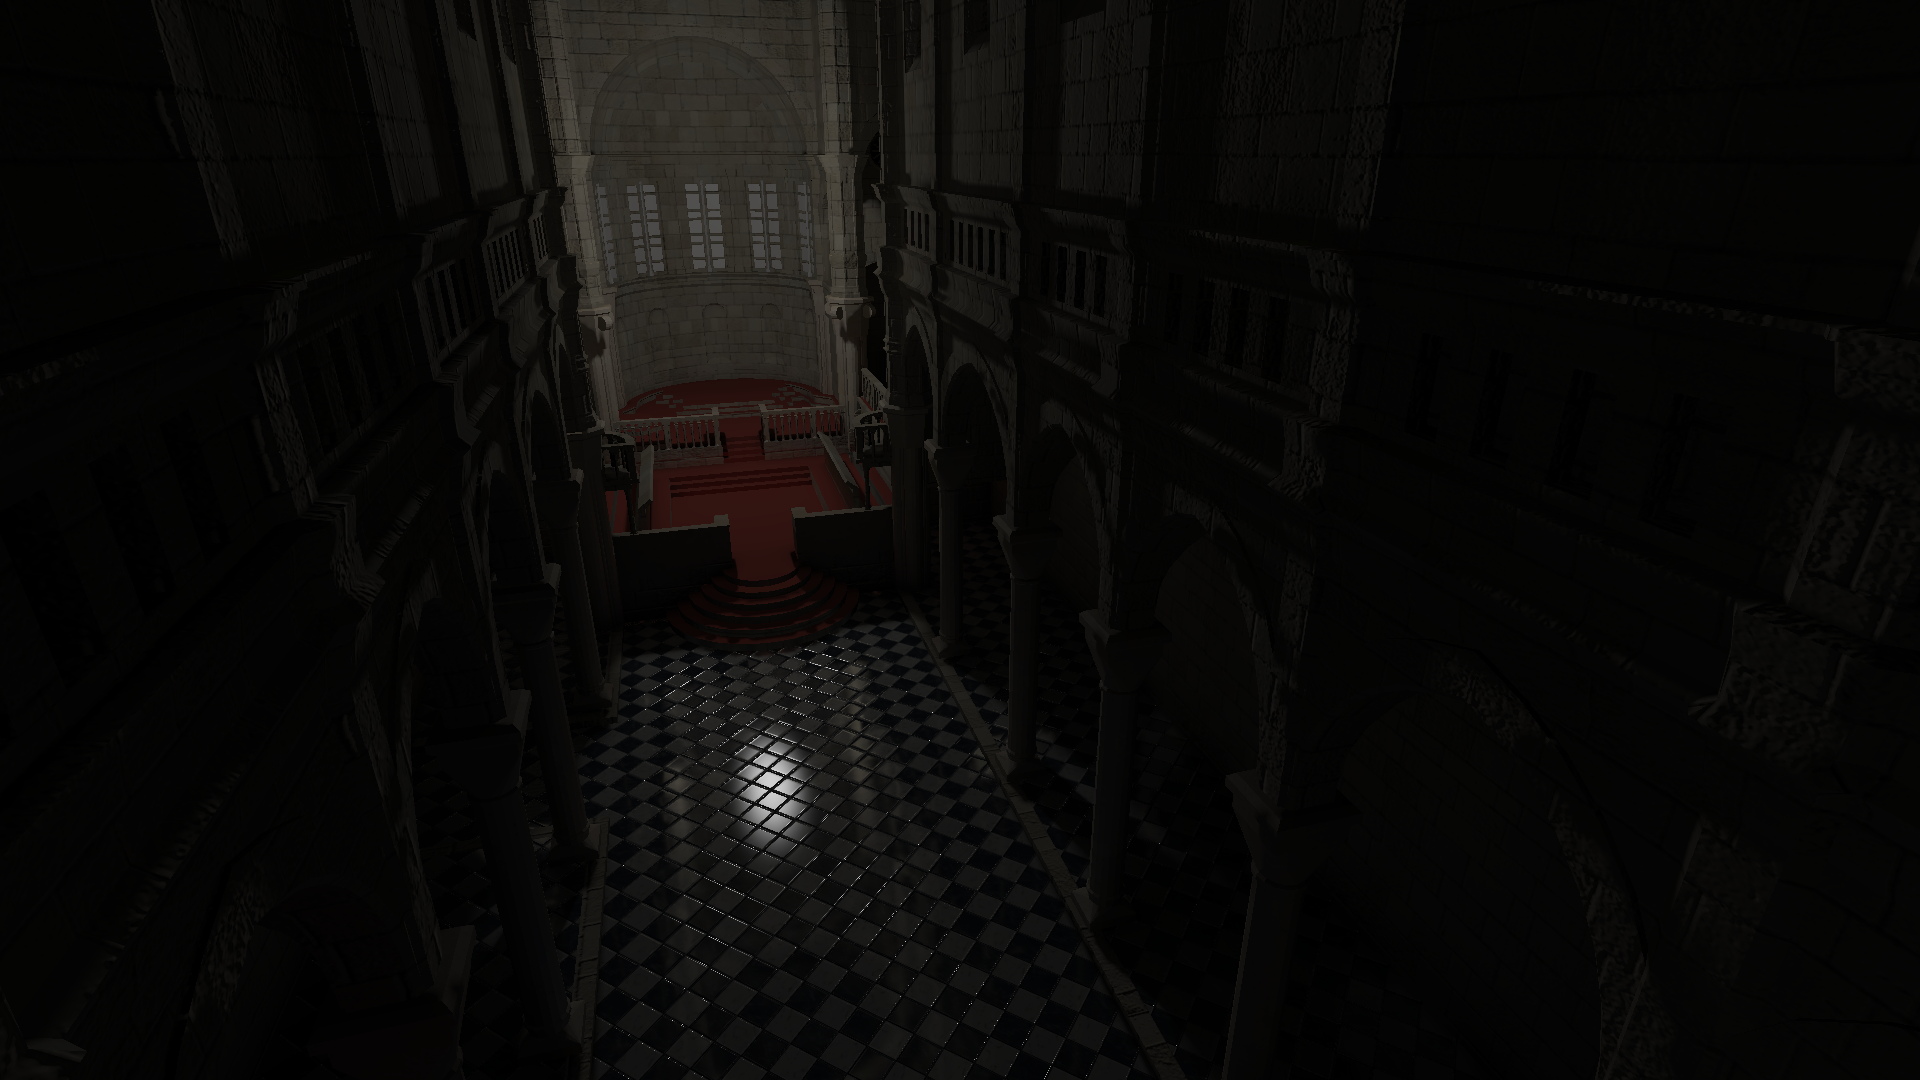
\includegraphics[width=\linewidth]{media/finals/sibenik_gi_256.png}
		%\caption*{$256^3$}
	\end{subfigure}%
	\hspace{0.01\textwidth}
	\begin{subfigure}[b]{.49\linewidth}
		\centering
		\captionsetup{justification=centering}
		%\caption*{Diferencia Perceptual\\}
		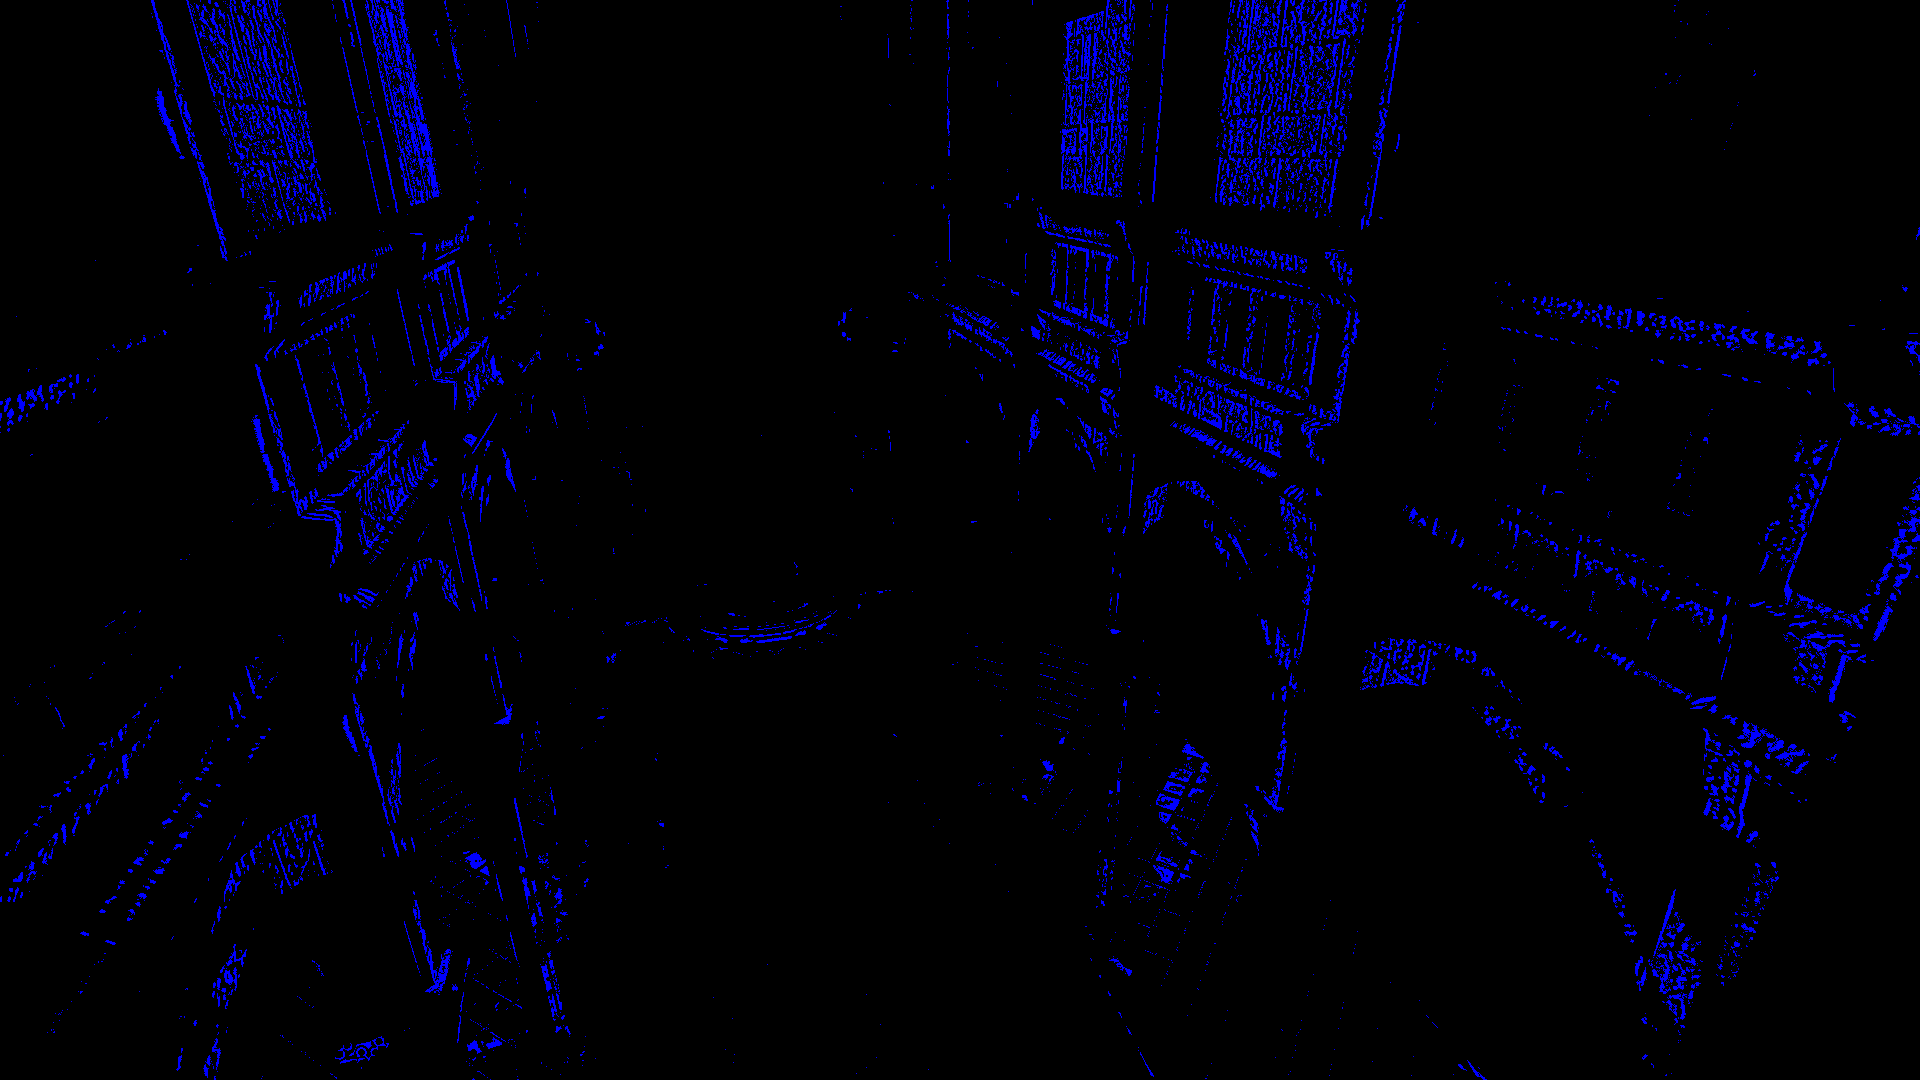
\includegraphics[width=\linewidth]{media/finals/sibenik_gi_256_diff.png}
		%\caption*{}
	\end{subfigure}%
	\par\smallskip
	\begin{subfigure}[b]{.49\linewidth}
		\centering
		\captionsetup{justification=centering}
		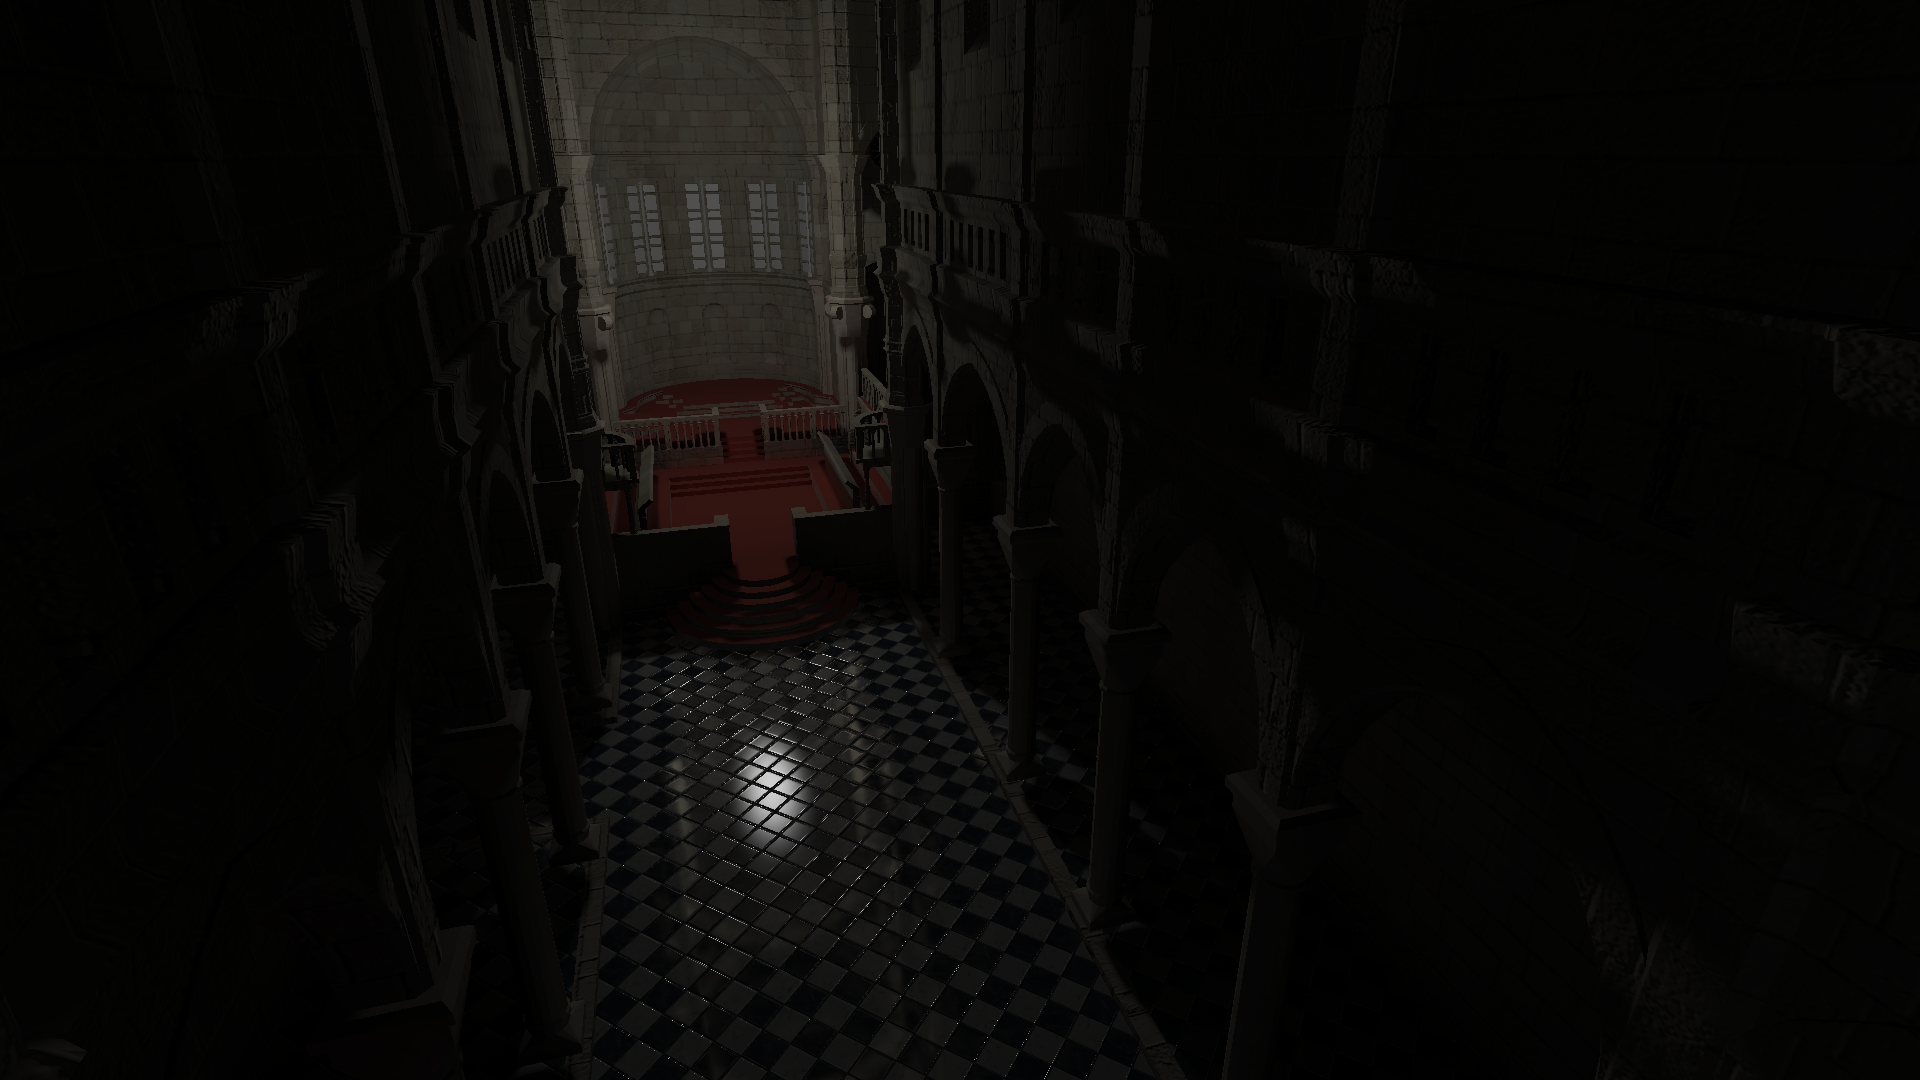
\includegraphics[width=\linewidth]{media/finals/sibenik_gi_128.png}
		%\caption*{$128^3$}
	\end{subfigure}%
	\hspace{0.01\textwidth}
	\begin{subfigure}[b]{.49\linewidth}
		\centering
		\captionsetup{justification=centering}
		%\caption*{Diferencia Perceptual}
		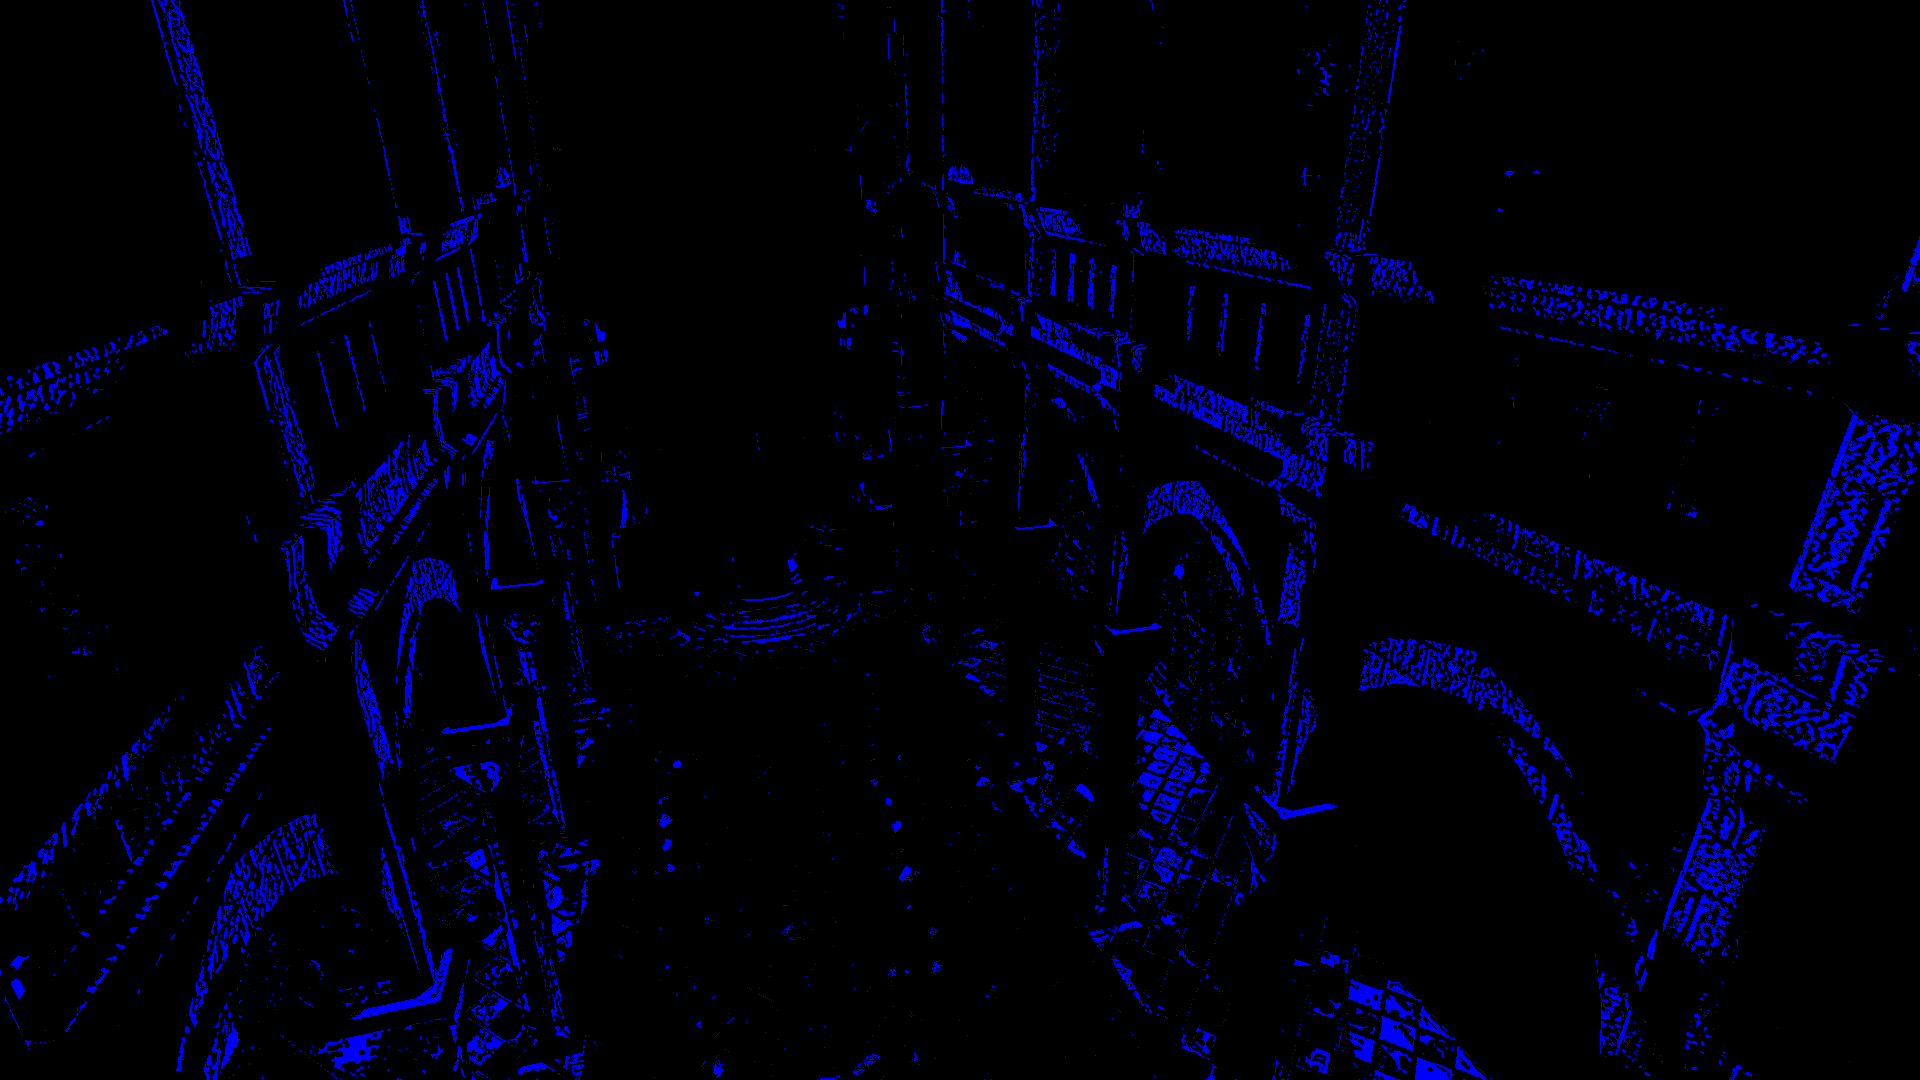
\includegraphics[width=\linewidth]{media/finals/sibenik_gi_128_diff.png}
		%\caption*{}
	\end{subfigure}%
	\par\smallskip
	\begin{subfigure}[b]{.49\linewidth}
		\centering
		\captionsetup{justification=centering}
		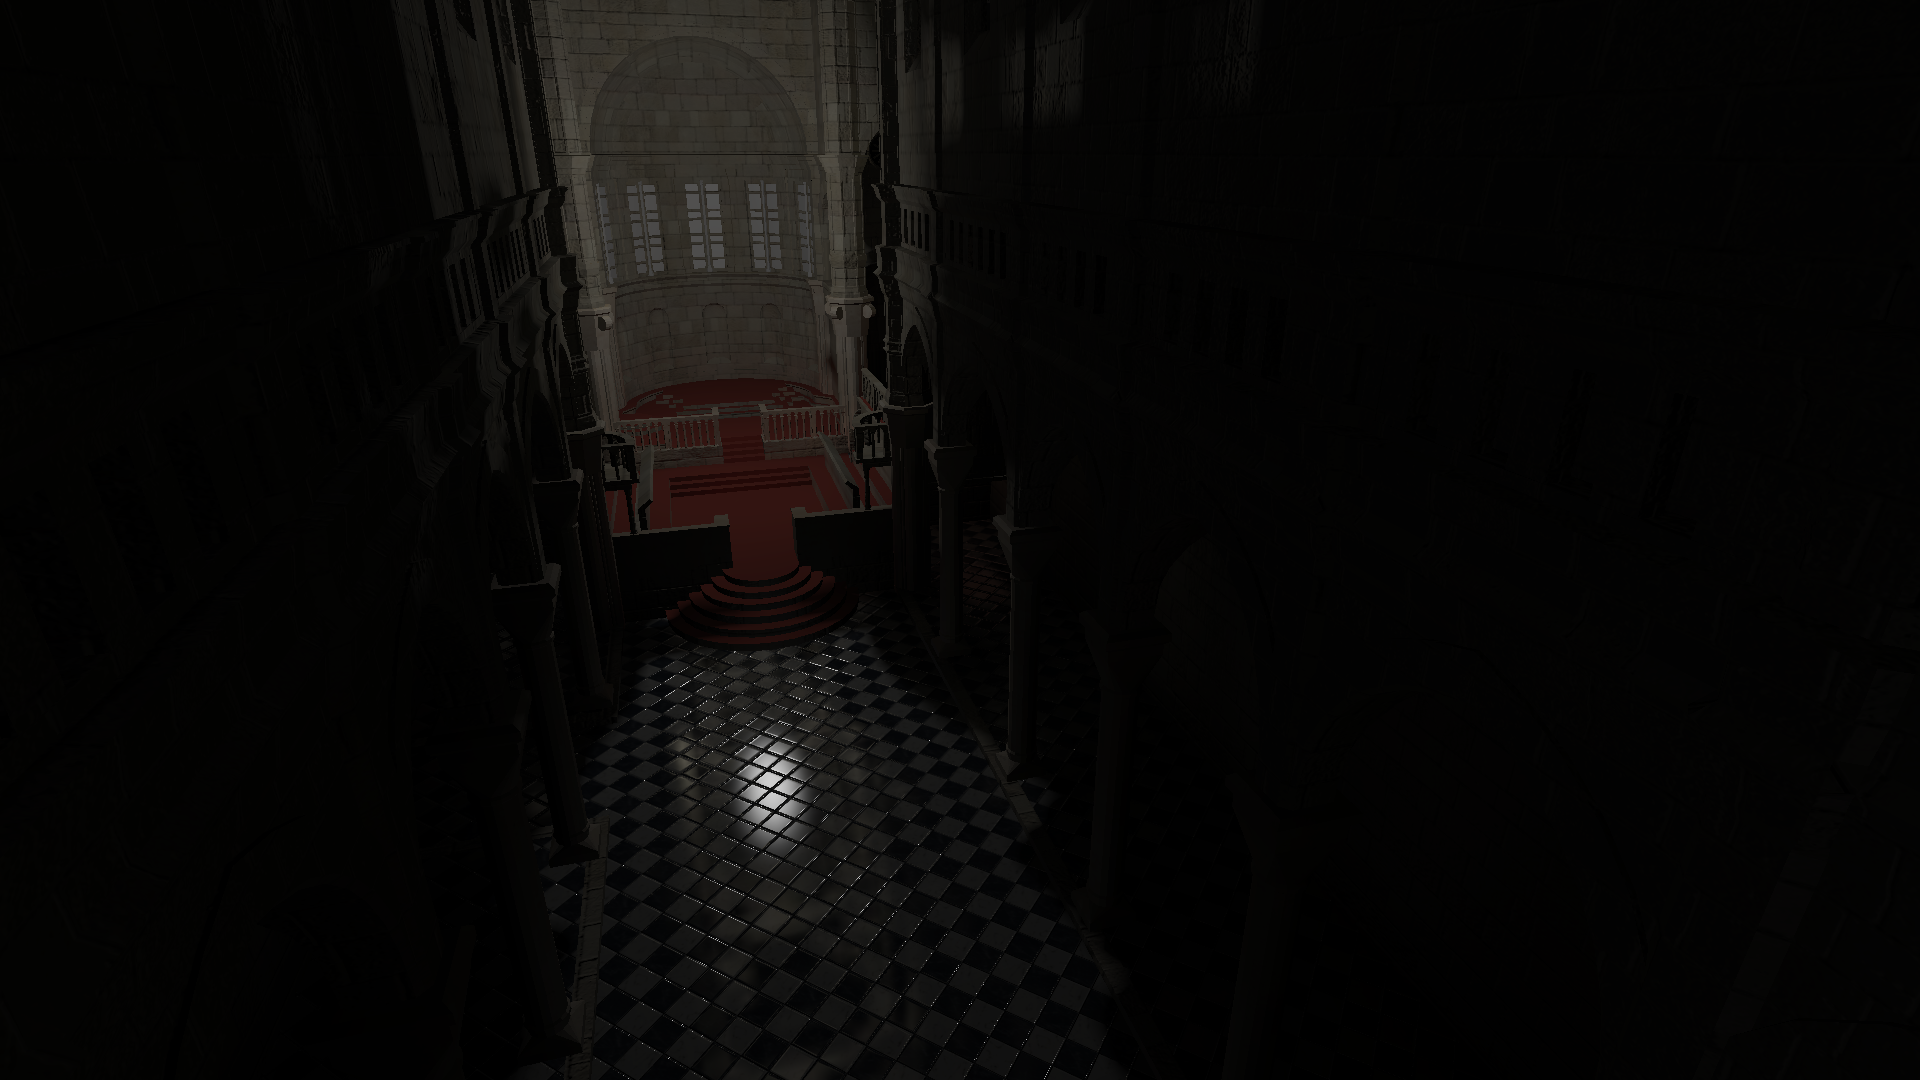
\includegraphics[width=\linewidth]{media/finals/sibenik_gi_64.png}
		%\caption*{$64^3$}
	\end{subfigure}%
	\hspace{0.01\textwidth}
	\begin{subfigure}[b]{.49\linewidth}
		\centering
		\captionsetup{justification=centering}
		%\caption*{Diferencia Perceptual}
		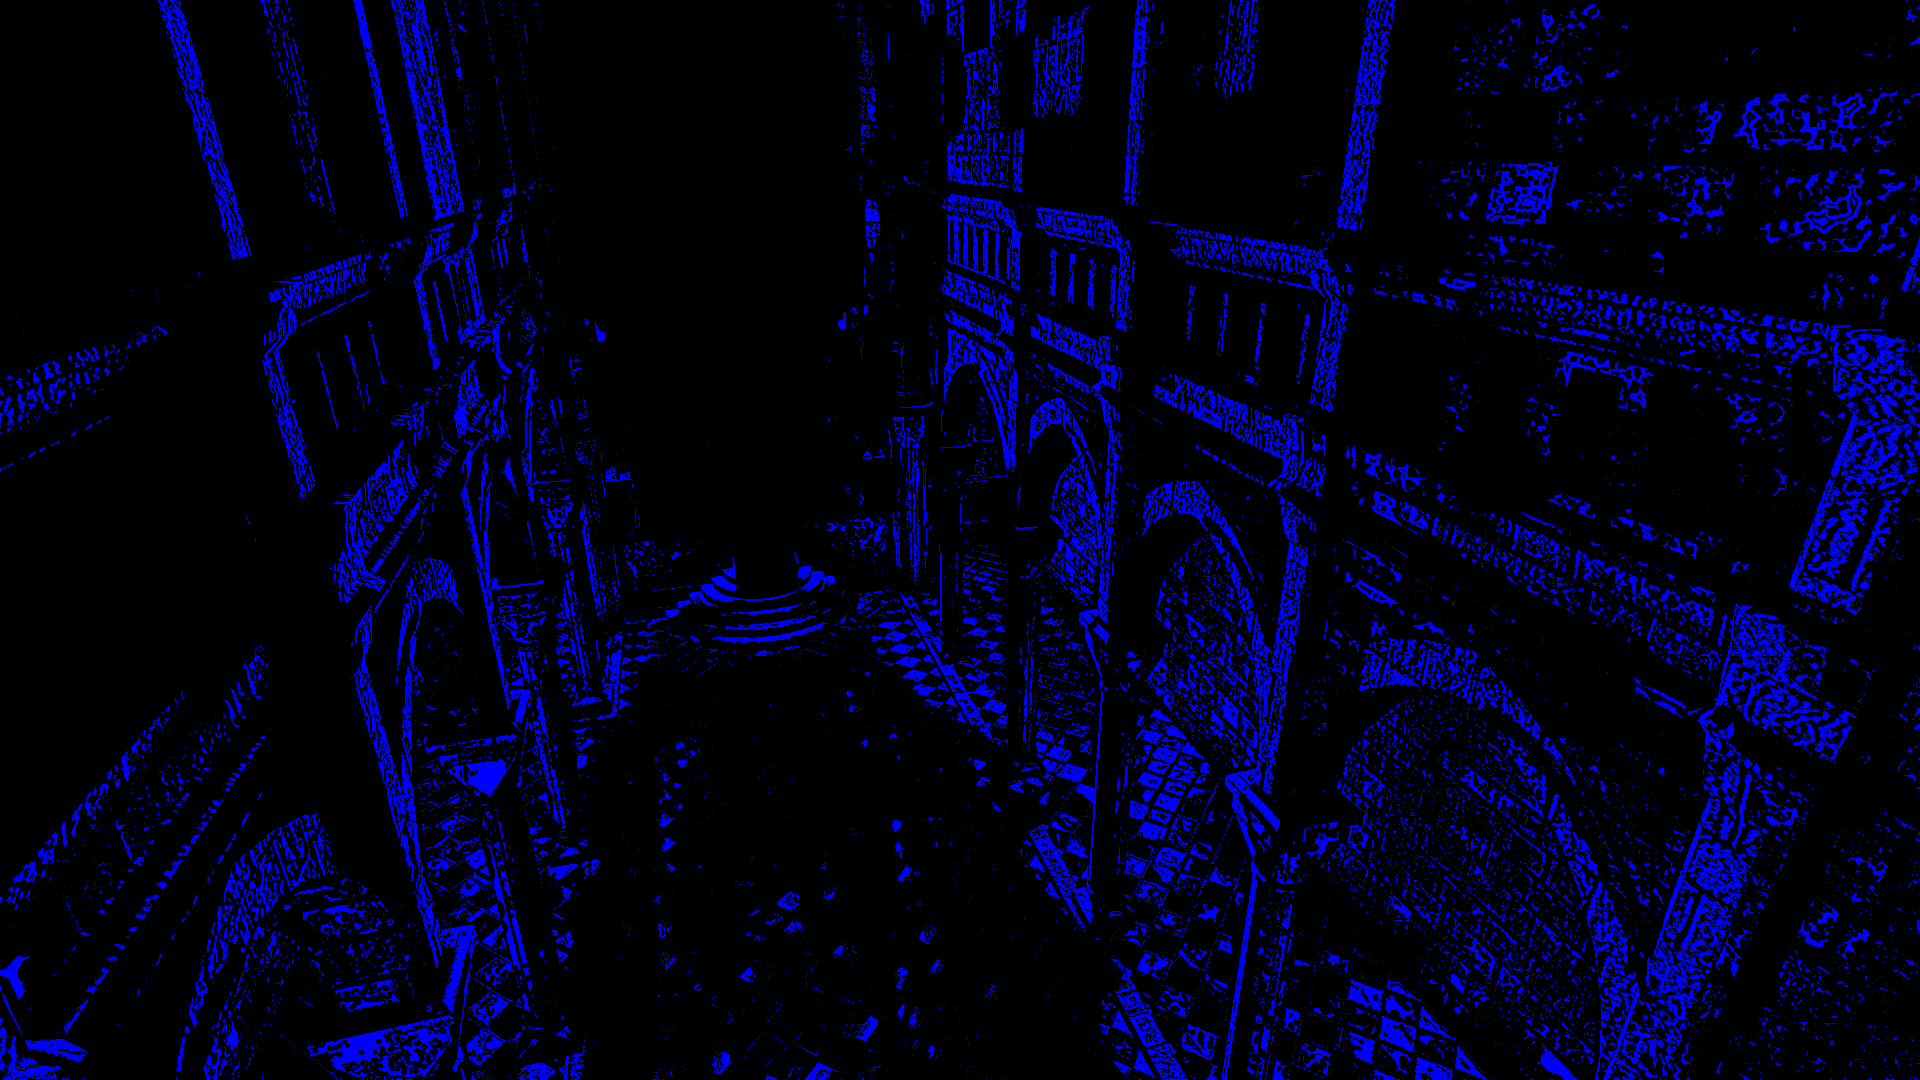
\includegraphics[width=\linewidth]{media/finals/sibenik_gi_64_diff.png}
		%\caption*{}
	\end{subfigure}%
	\caption{Diferencia visual con respecto a la imagen \ref{fig:sibenik_final} utilizando distintas resoluciones para la representación en vóxeles.}
	\label{fig:sibenik_gi_resdiff}
\end{figure}

\begin{figure}[H]
	\centering
	\begin{subfigure}[b]{.49\linewidth}
		\centering
		\captionsetup{justification=centering}
		%\caption*{Directa, Indirecta y Oclusión Ambiental}
		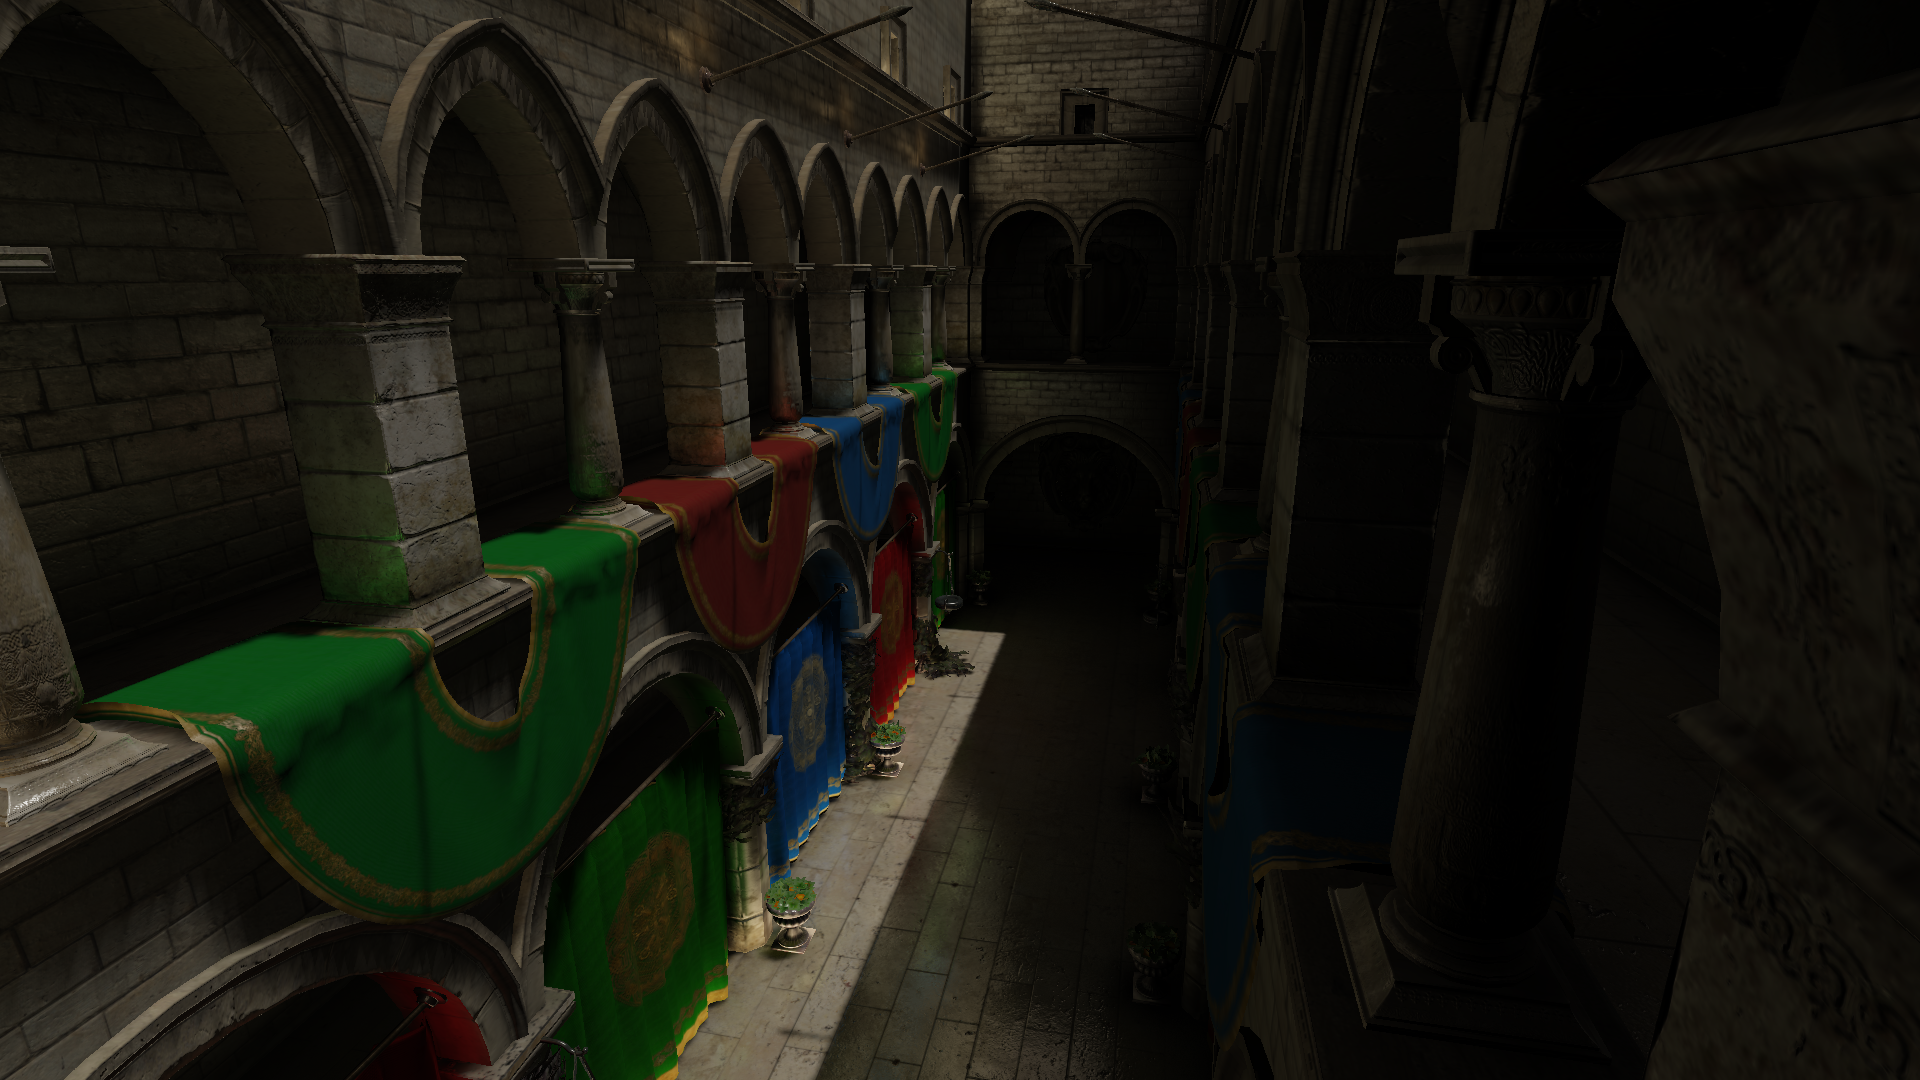
\includegraphics[width=\linewidth]{media/finals/sponza_gi_256.png}
		%\caption*{$256^3$}
	\end{subfigure}%
	\hspace{0.01\textwidth}
	\begin{subfigure}[b]{.49\linewidth}
		\centering
		\captionsetup{justification=centering}
		%\caption*{Diferencia Perceptual\\}
		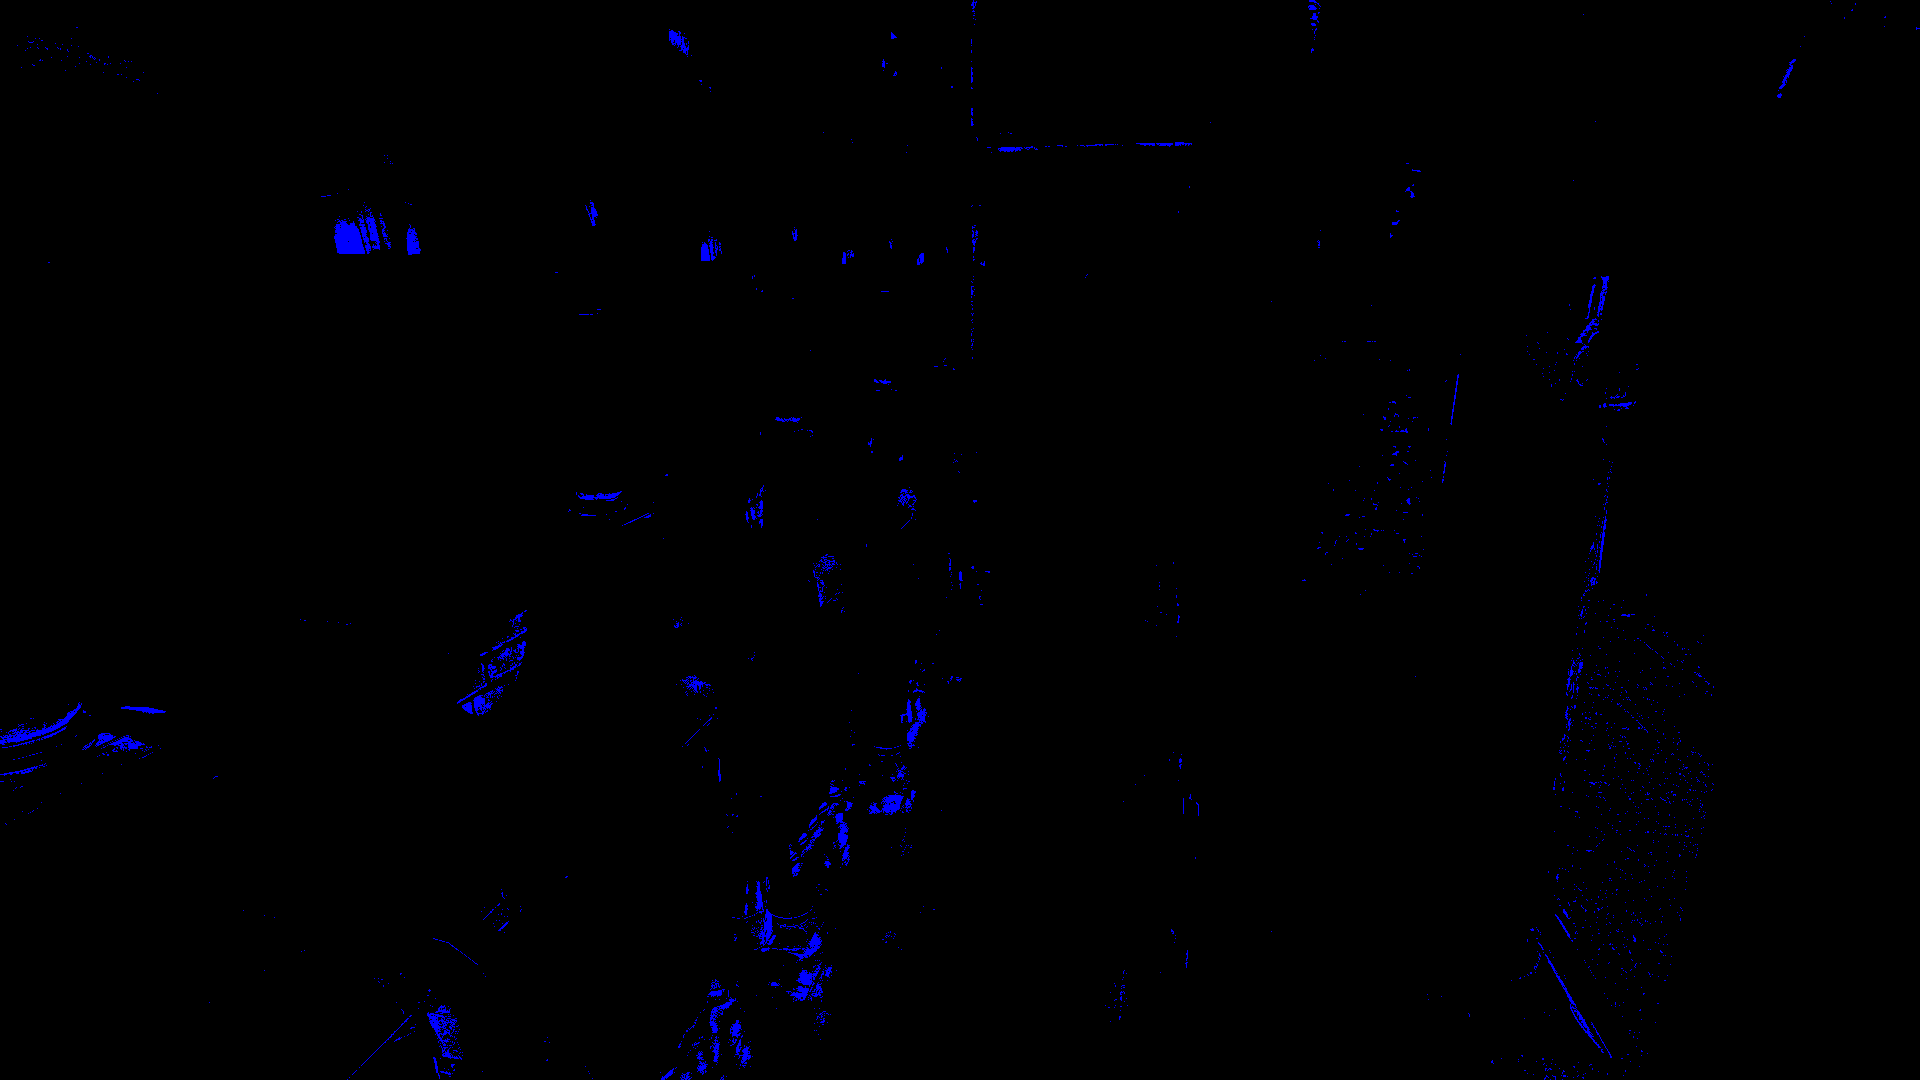
\includegraphics[width=\linewidth]{media/finals/sponza_gi_256_diff.png}
		%\caption*{}
	\end{subfigure}%
	\par\smallskip
	\begin{subfigure}[b]{.49\linewidth}
		\centering
		\captionsetup{justification=centering}
		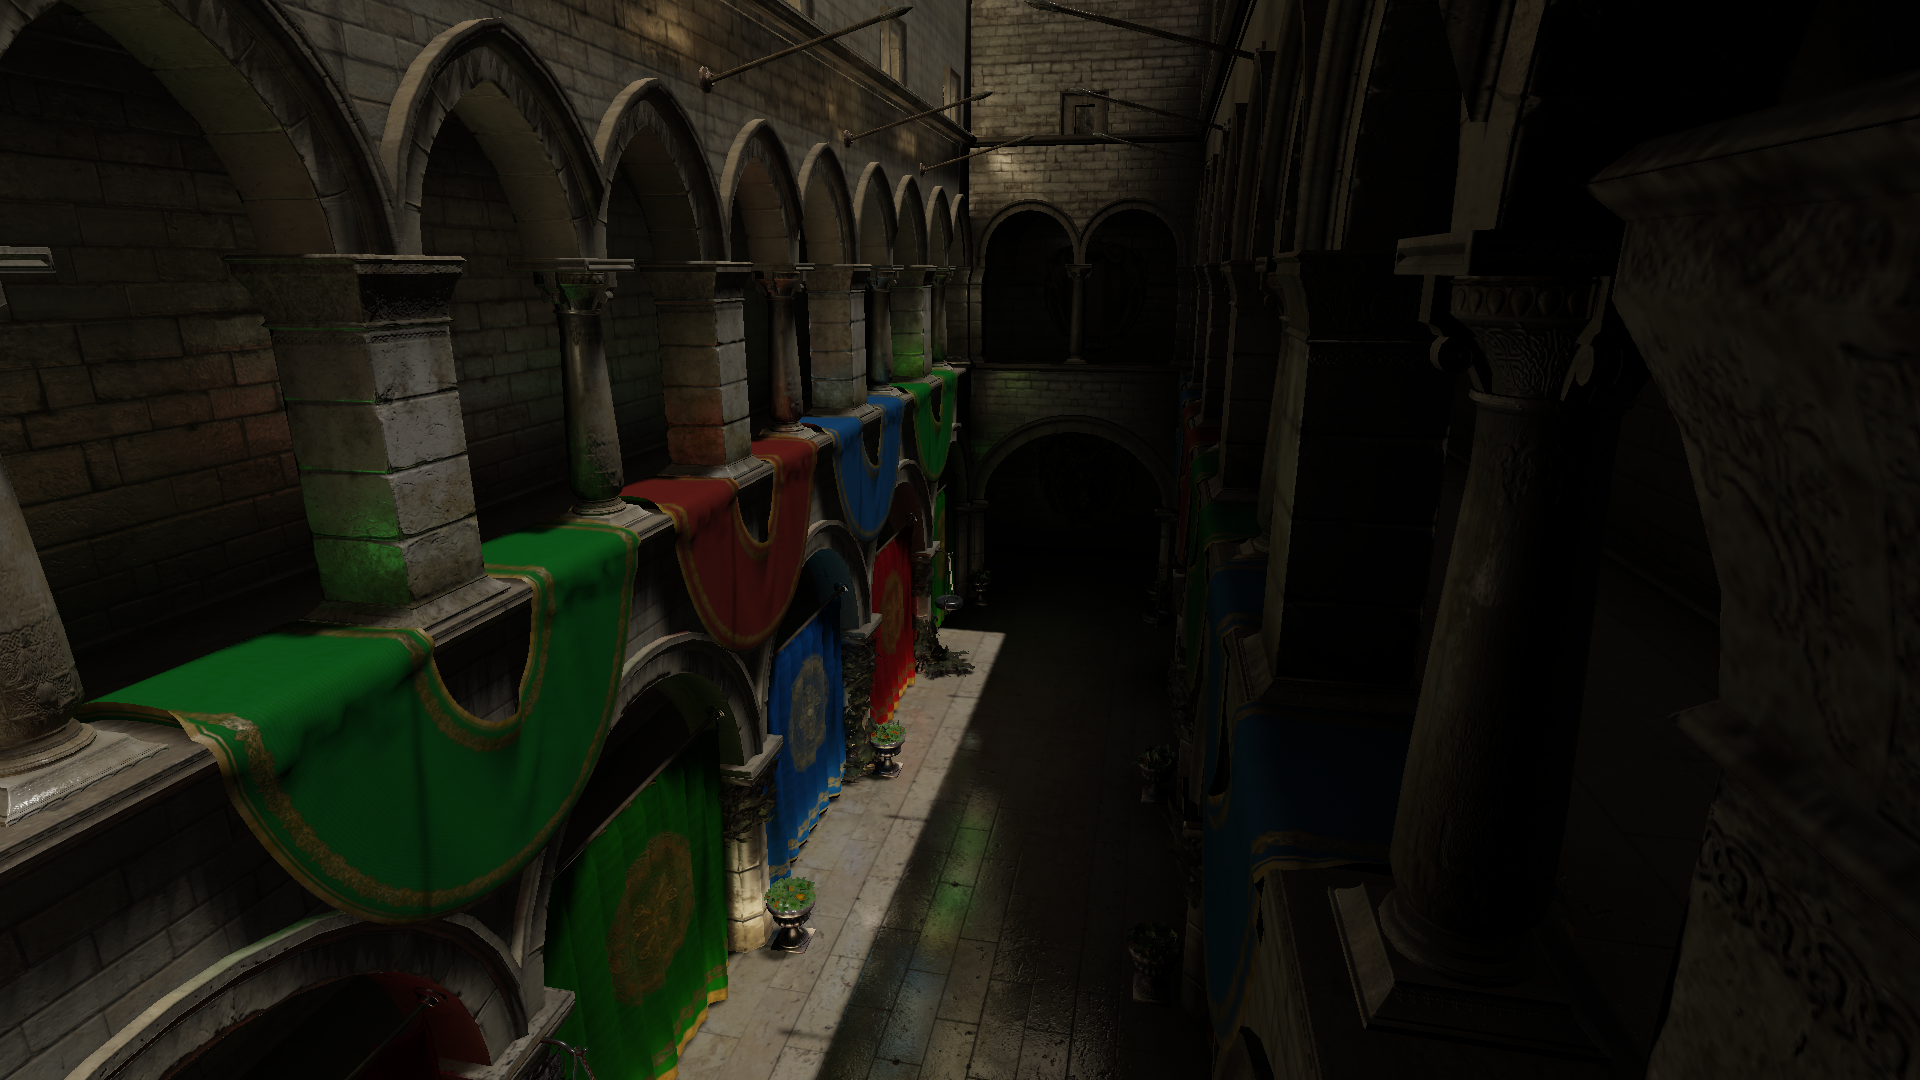
\includegraphics[width=\linewidth]{media/finals/sponza_gi_128.png}
		%\caption*{$128^3$}
	\end{subfigure}%
	\hspace{0.01\textwidth}
	\begin{subfigure}[b]{.49\linewidth}
		\centering
		\captionsetup{justification=centering}
		%\caption*{Diferencia Perceptual}
		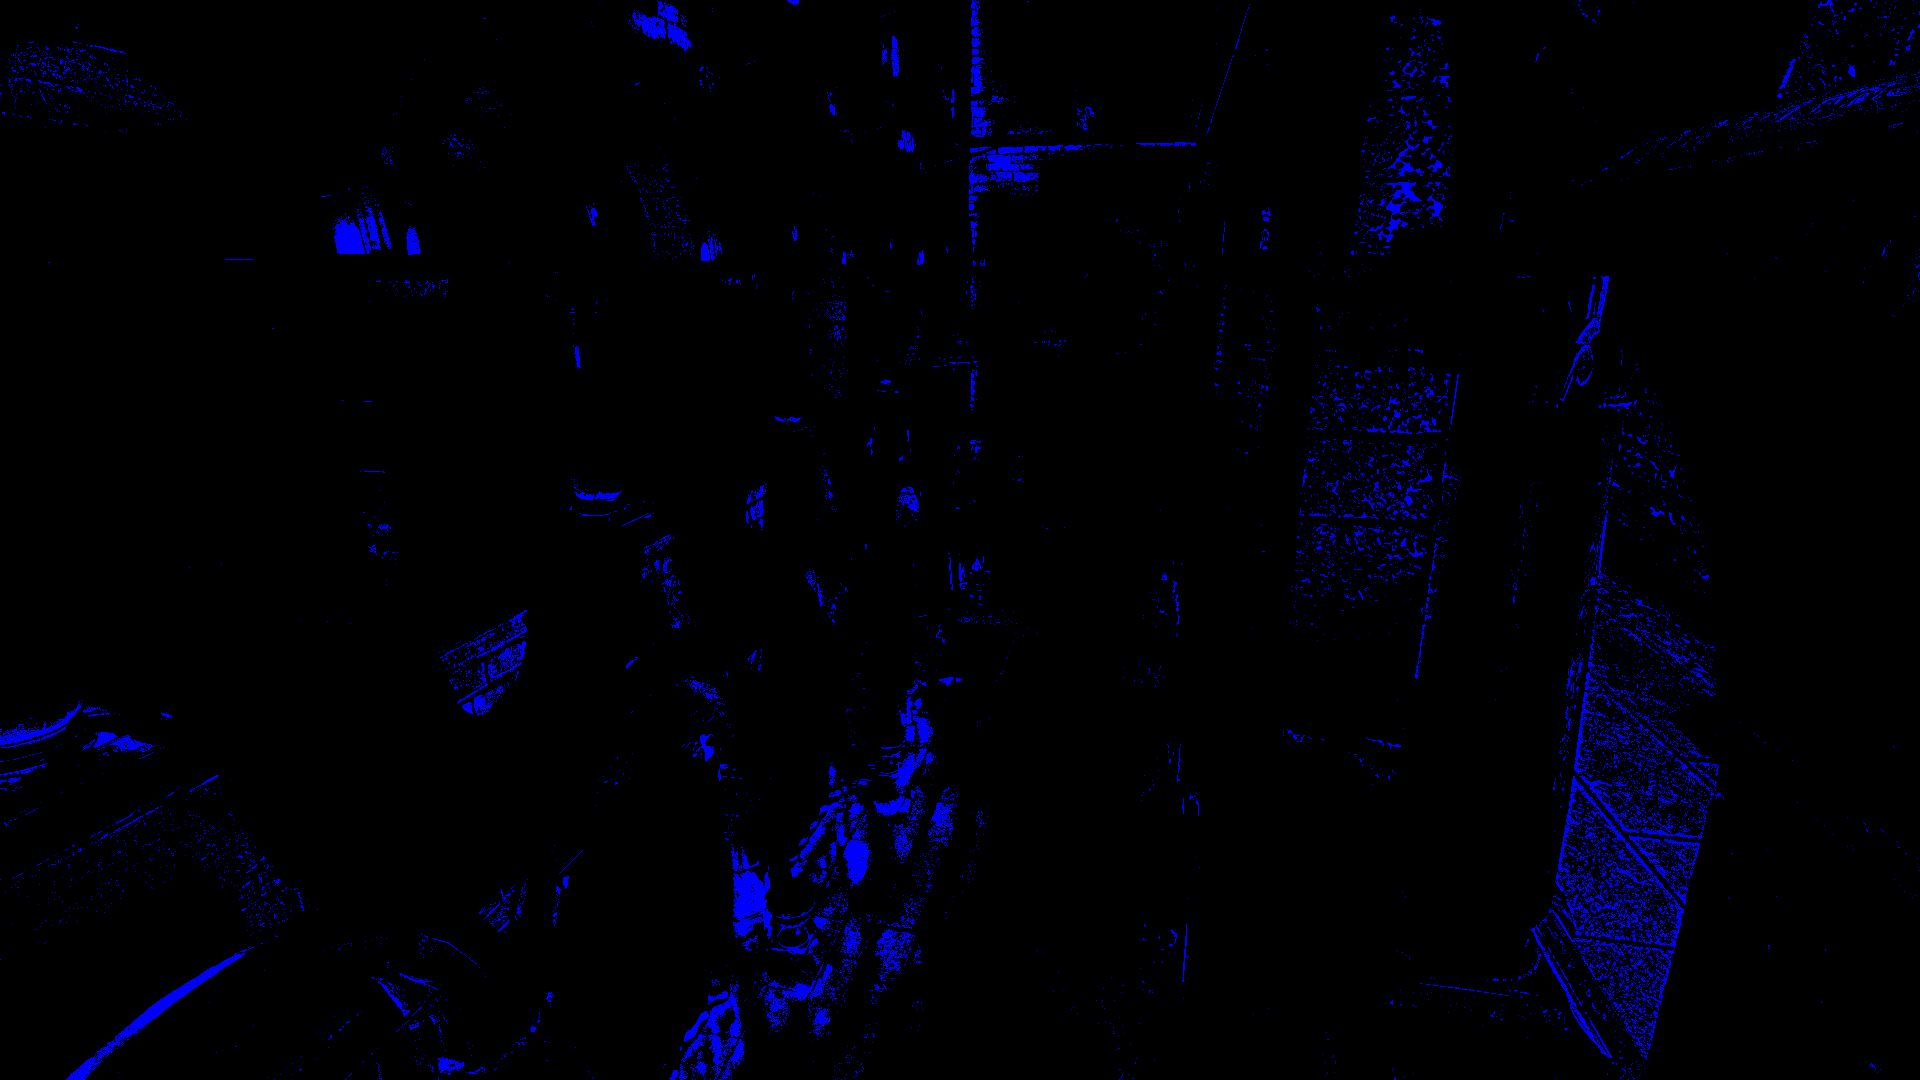
\includegraphics[width=\linewidth]{media/finals/sponza_gi_128_diff.png}
		%\caption*{}
	\end{subfigure}%
	\par\smallskip
	\begin{subfigure}[b]{.49\linewidth}
		\centering
		\captionsetup{justification=centering}
		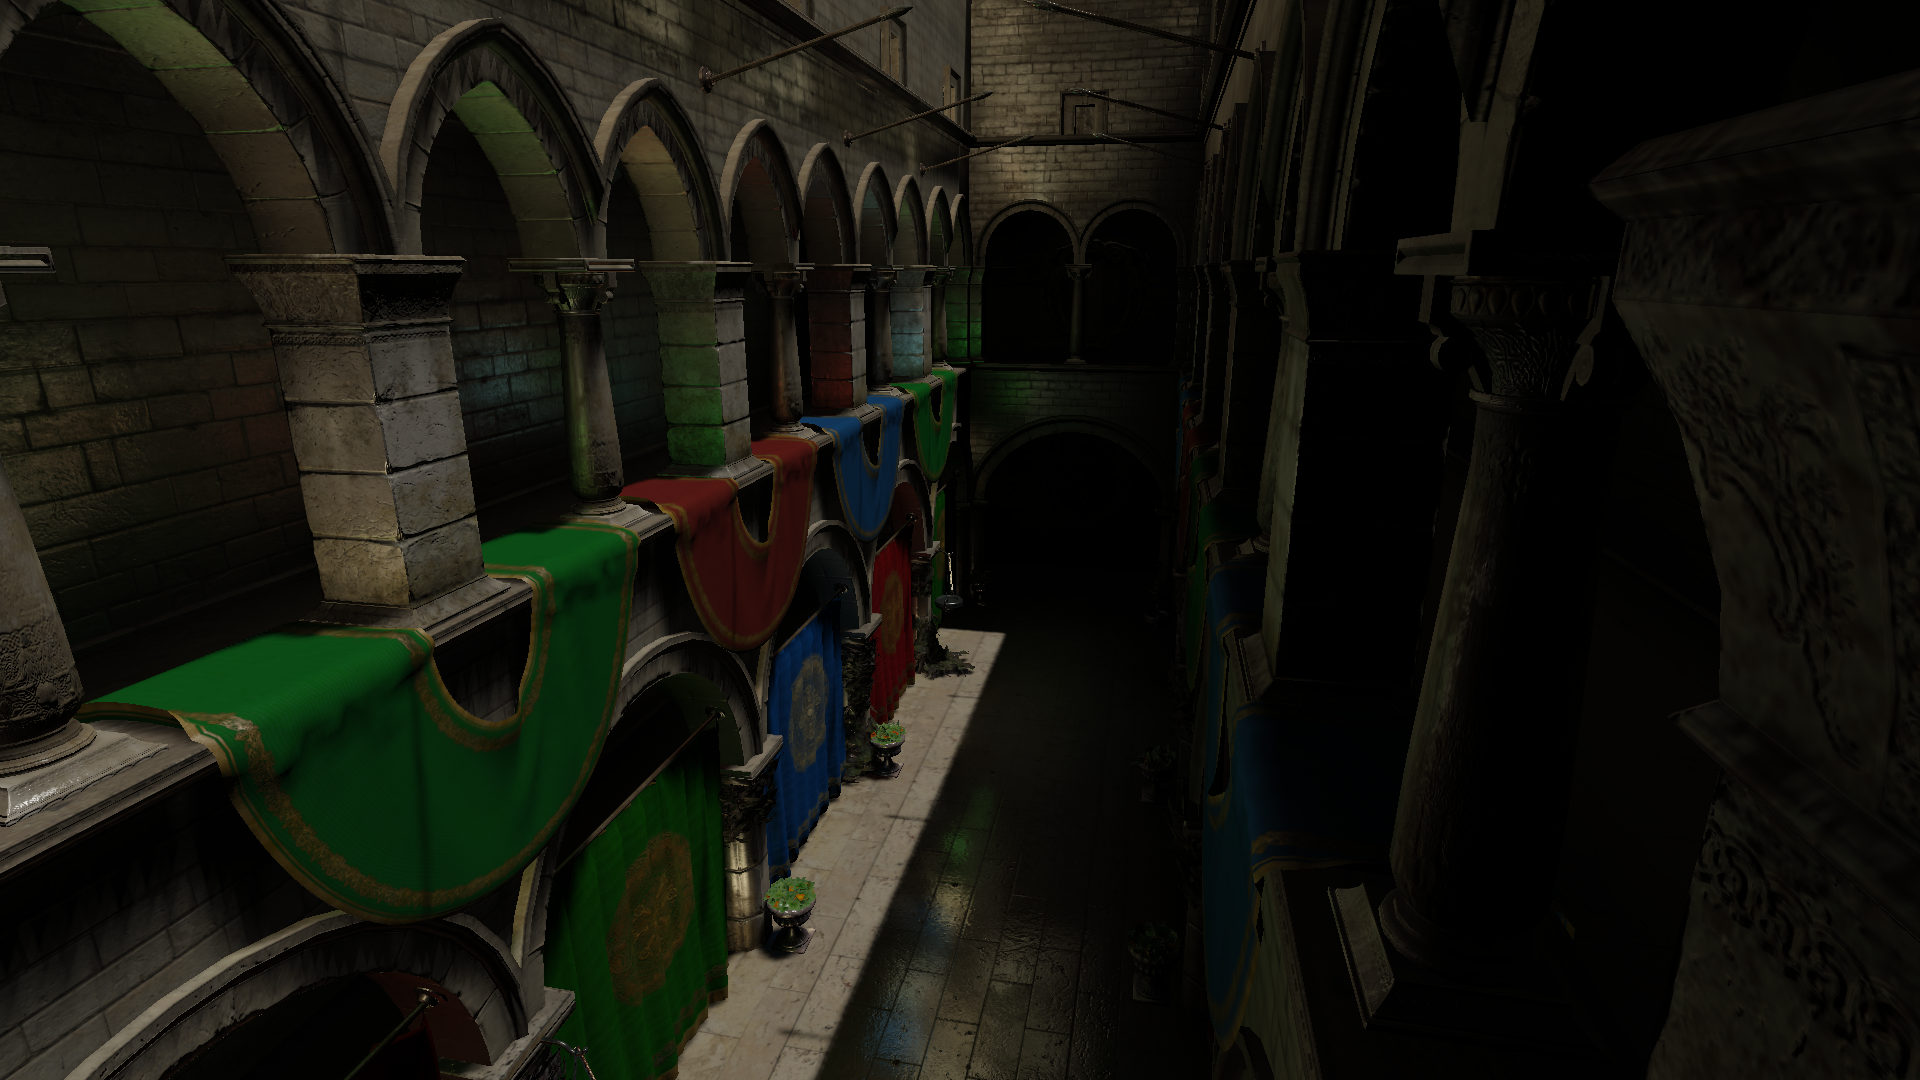
\includegraphics[width=\linewidth]{media/finals/sponza_gi_64.png}
		%\caption*{$64^3$}
	\end{subfigure}%
	\hspace{0.01\textwidth}
	\begin{subfigure}[b]{.49\linewidth}
		\centering
		\captionsetup{justification=centering}
		%\caption*{Diferencia Perceptual}
		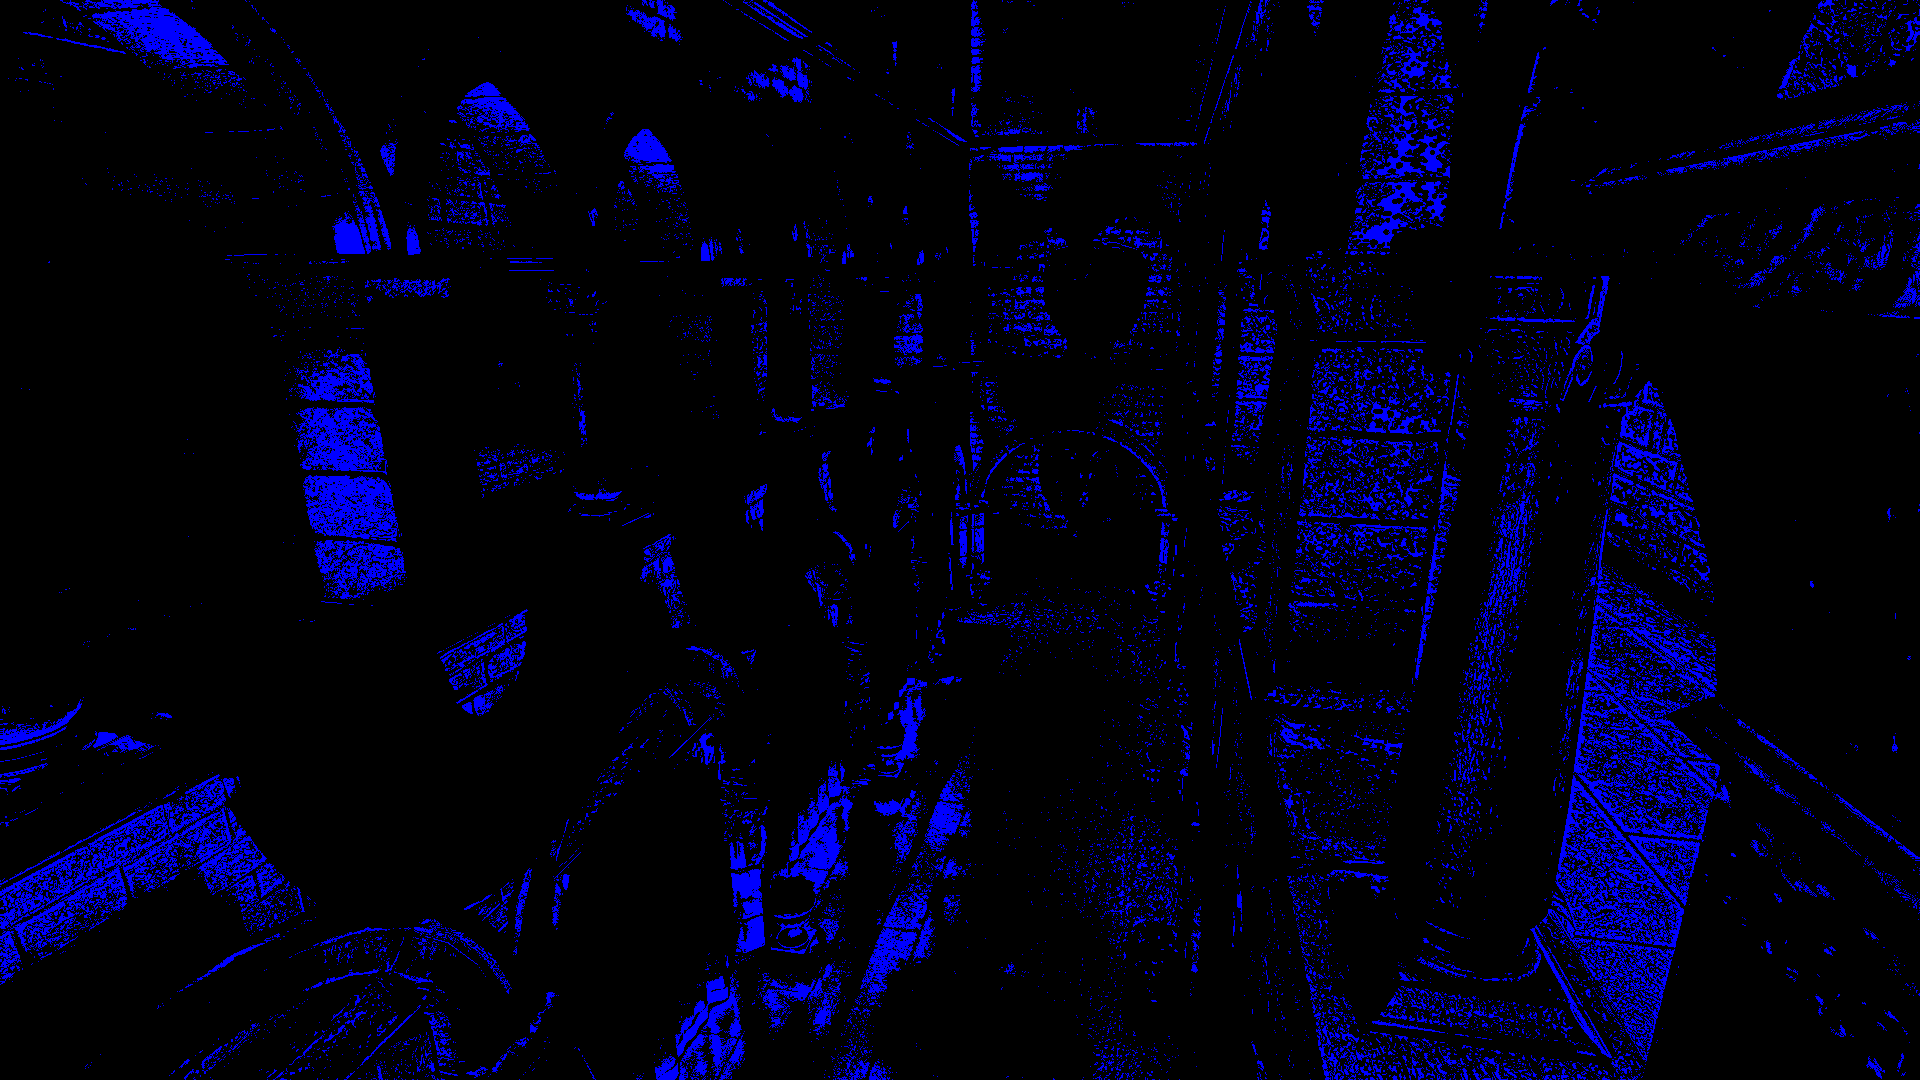
\includegraphics[width=\linewidth]{media/finals/sponza_gi_64_diff.png}
		%\caption*{}
	\end{subfigure}%
	\caption{Diferencia visual con respecto a la imagen \ref{fig:sponza_final} utilizando distintas resoluciones para la representación en vóxeles.}
	\label{fig:sponza_gi_resdiff}
\end{figure}

\begin{figure}[H]
	\centering
	\begin{subfigure}[b]{.49\linewidth}
		\centering
		\captionsetup{justification=centering}
		%\caption*{Directa, Indirecta y Oclusión Ambiental}
		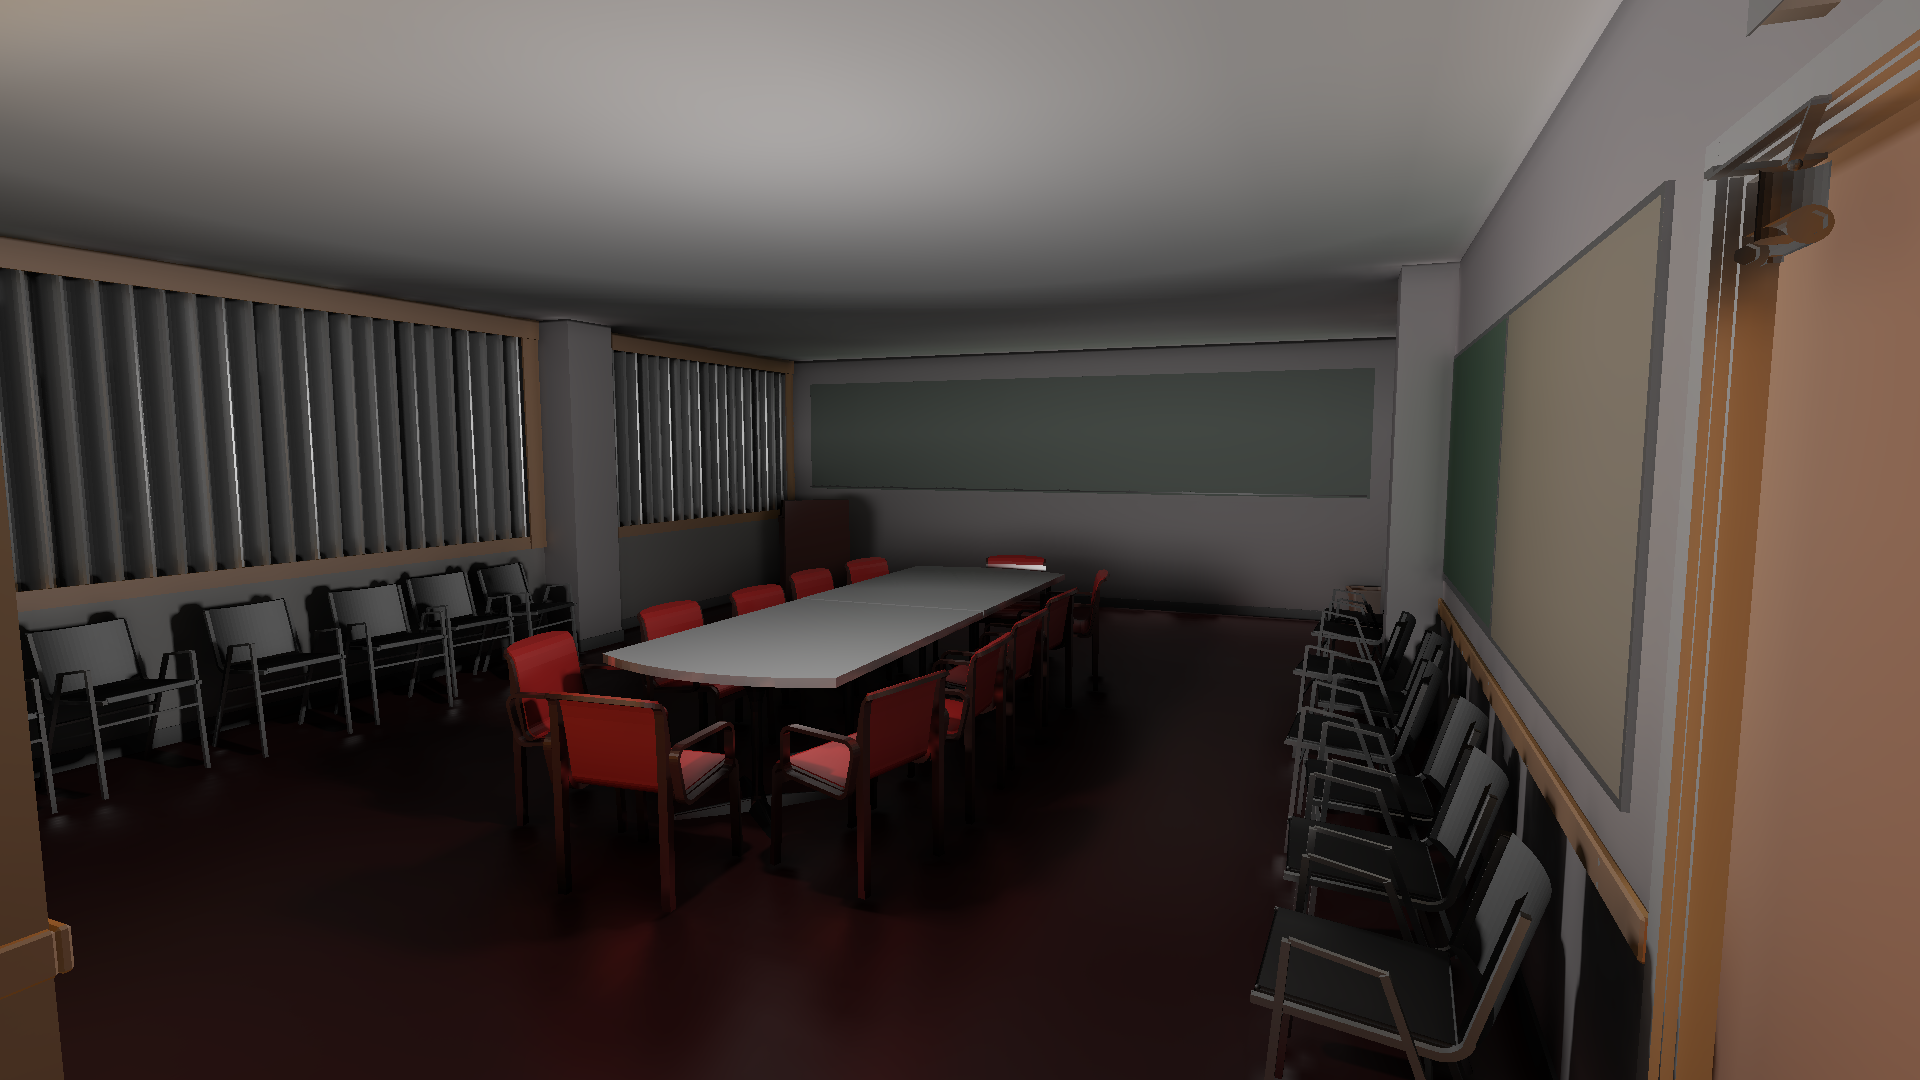
\includegraphics[width=\linewidth]{media/finals/conf_gi_256.png}
		%\caption*{$256^3$}
	\end{subfigure}%
	\hspace{0.01\textwidth}
	\begin{subfigure}[b]{.49\linewidth}
		\centering
		\captionsetup{justification=centering}
		%\caption*{Diferencia Perceptual\\}
		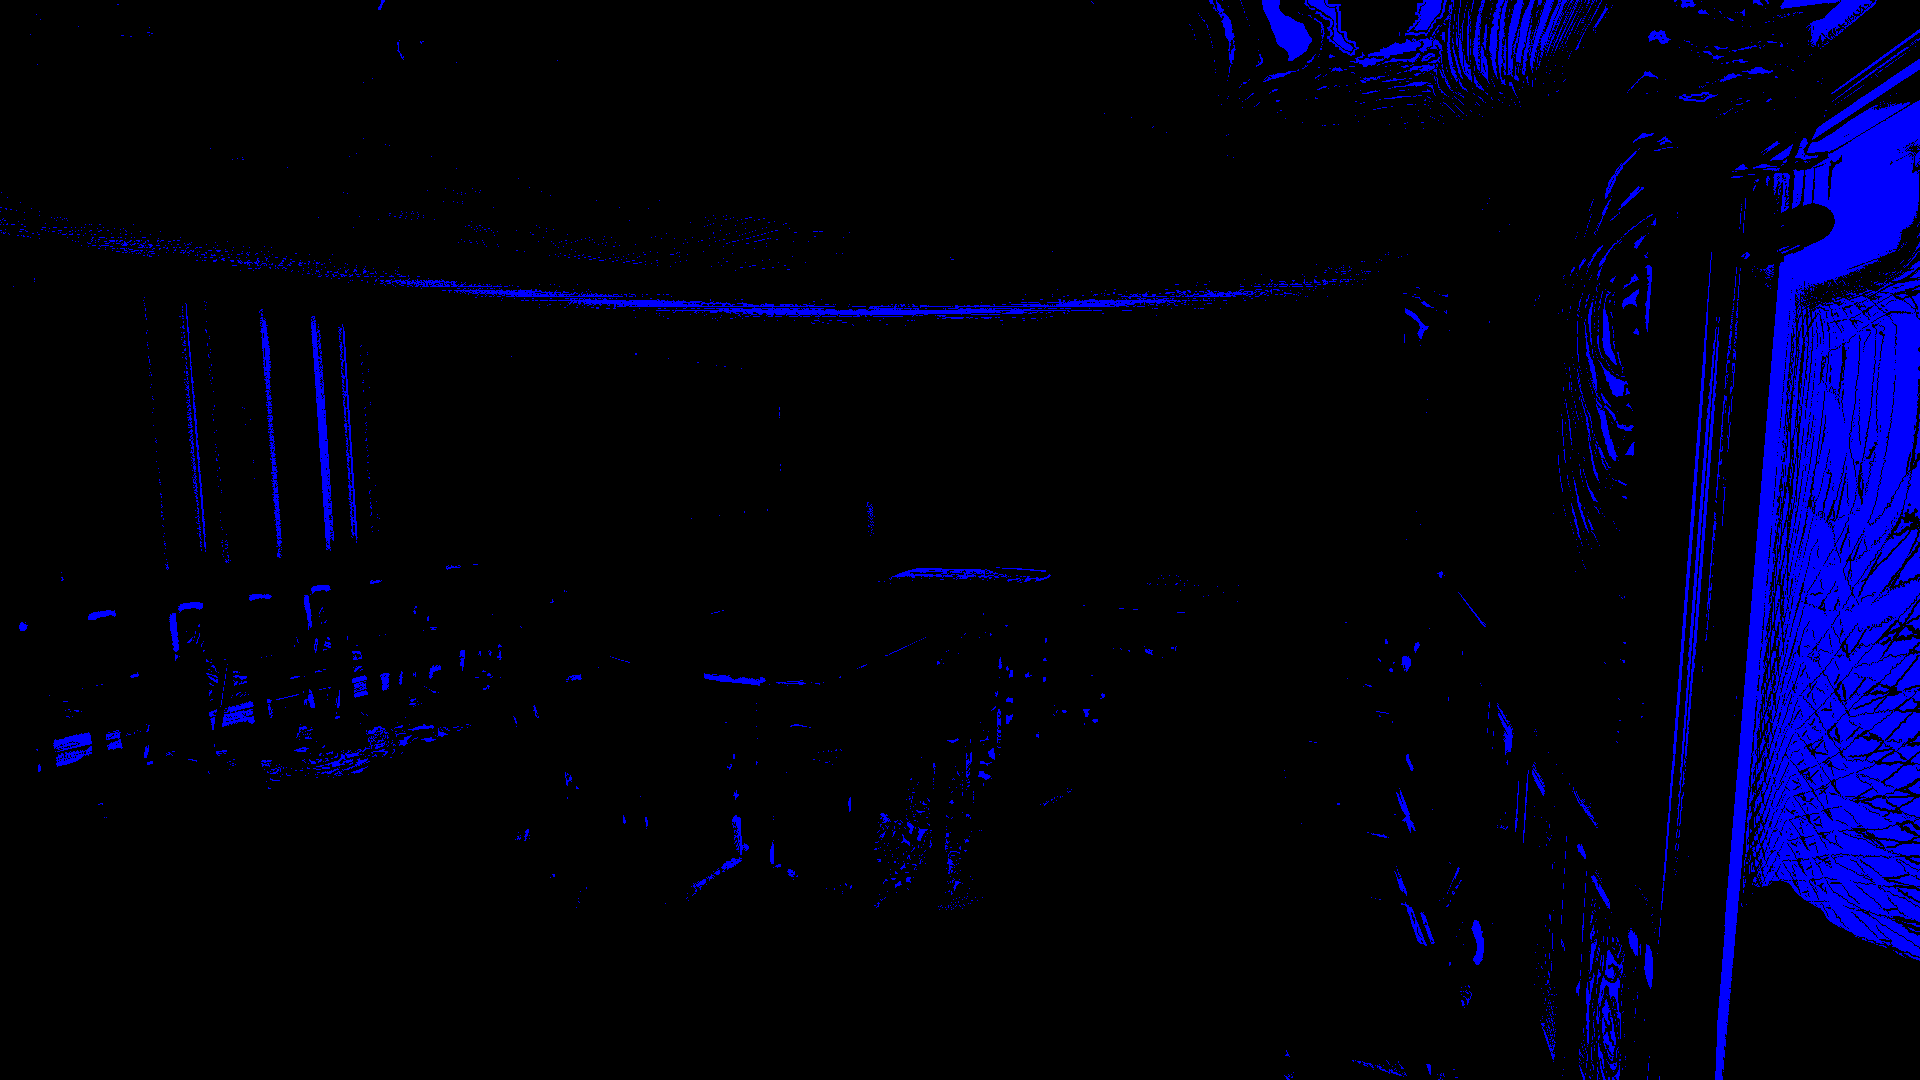
\includegraphics[width=\linewidth]{media/finals/conf_gi_256_diff.png}
		%\caption*{}
	\end{subfigure}%
	\par\smallskip
	\begin{subfigure}[b]{.49\linewidth}
		\centering
		\captionsetup{justification=centering}
		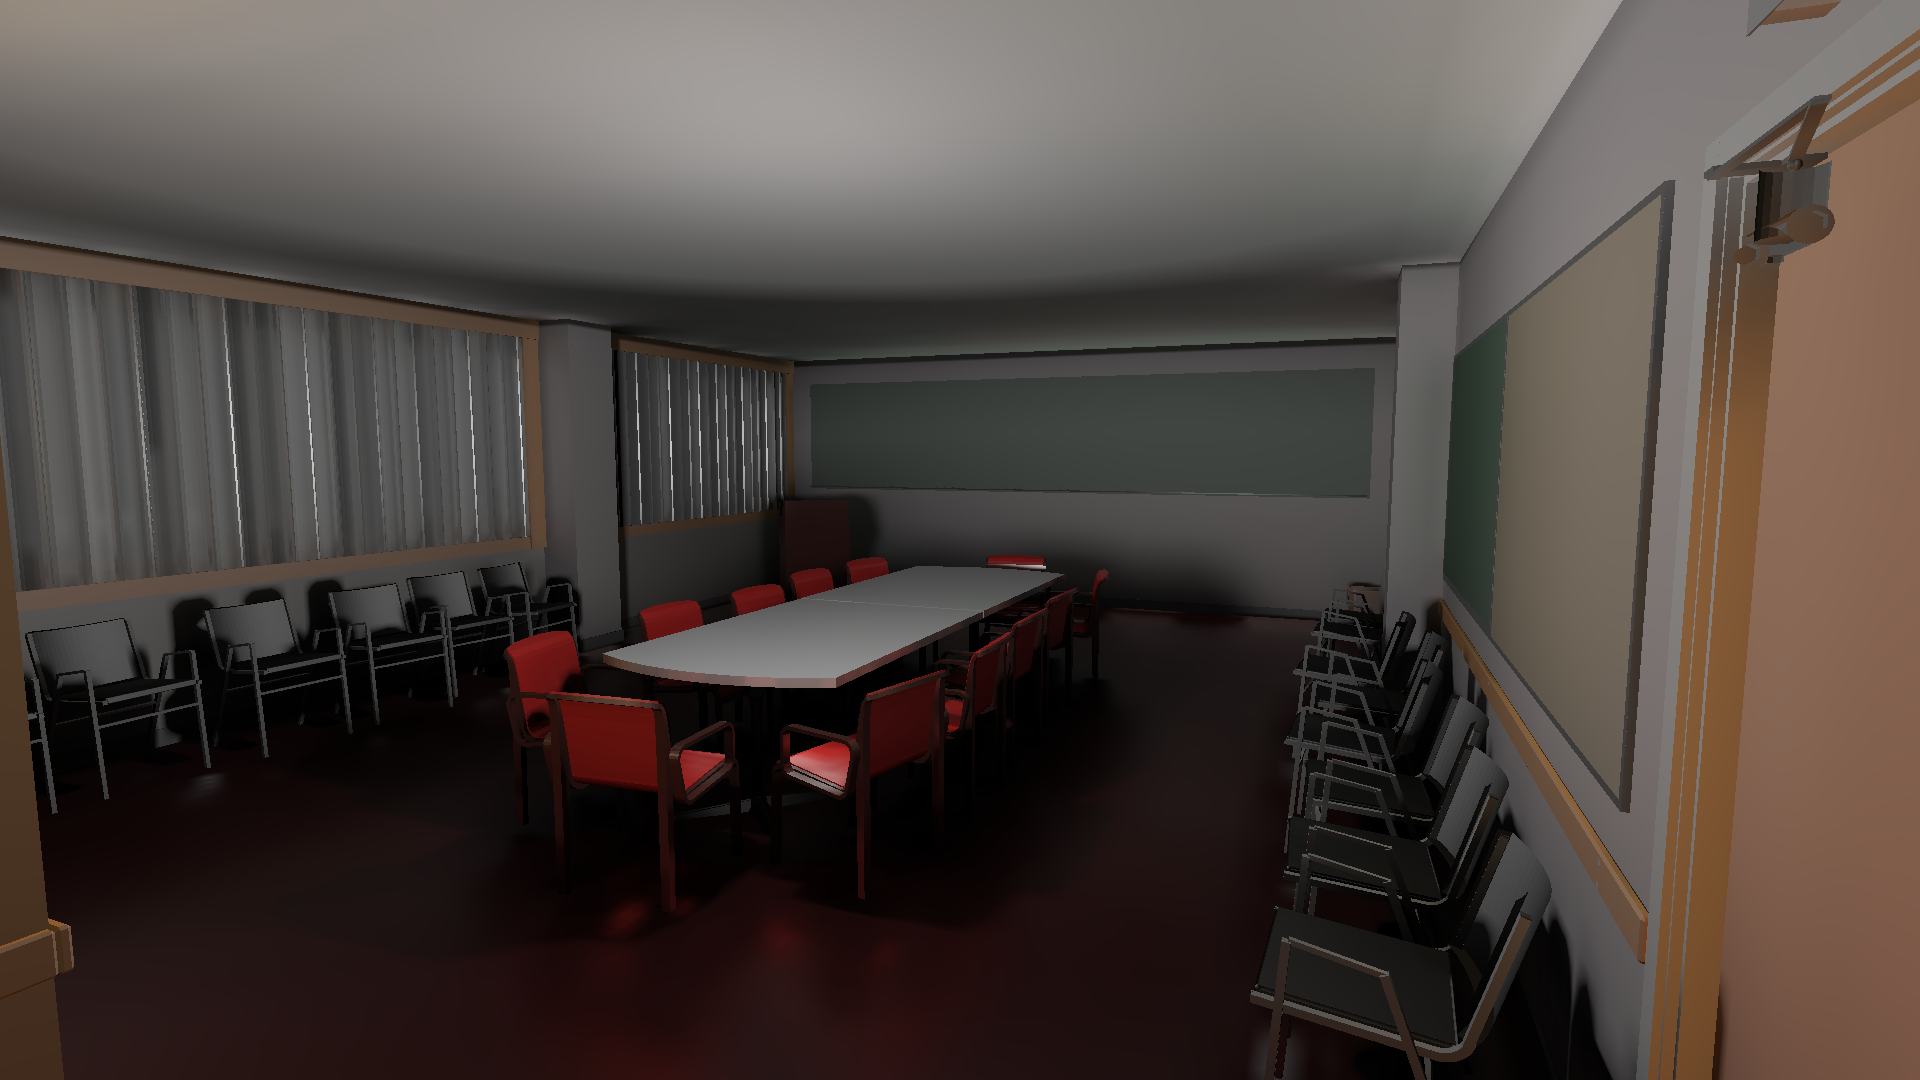
\includegraphics[width=\linewidth]{media/finals/conf_gi_128.png}
		%\caption*{$128^3$}
	\end{subfigure}%
	\hspace{0.01\textwidth}
	\begin{subfigure}[b]{.49\linewidth}
		\centering
		\captionsetup{justification=centering}
		%\caption*{Diferencia Perceptual}
		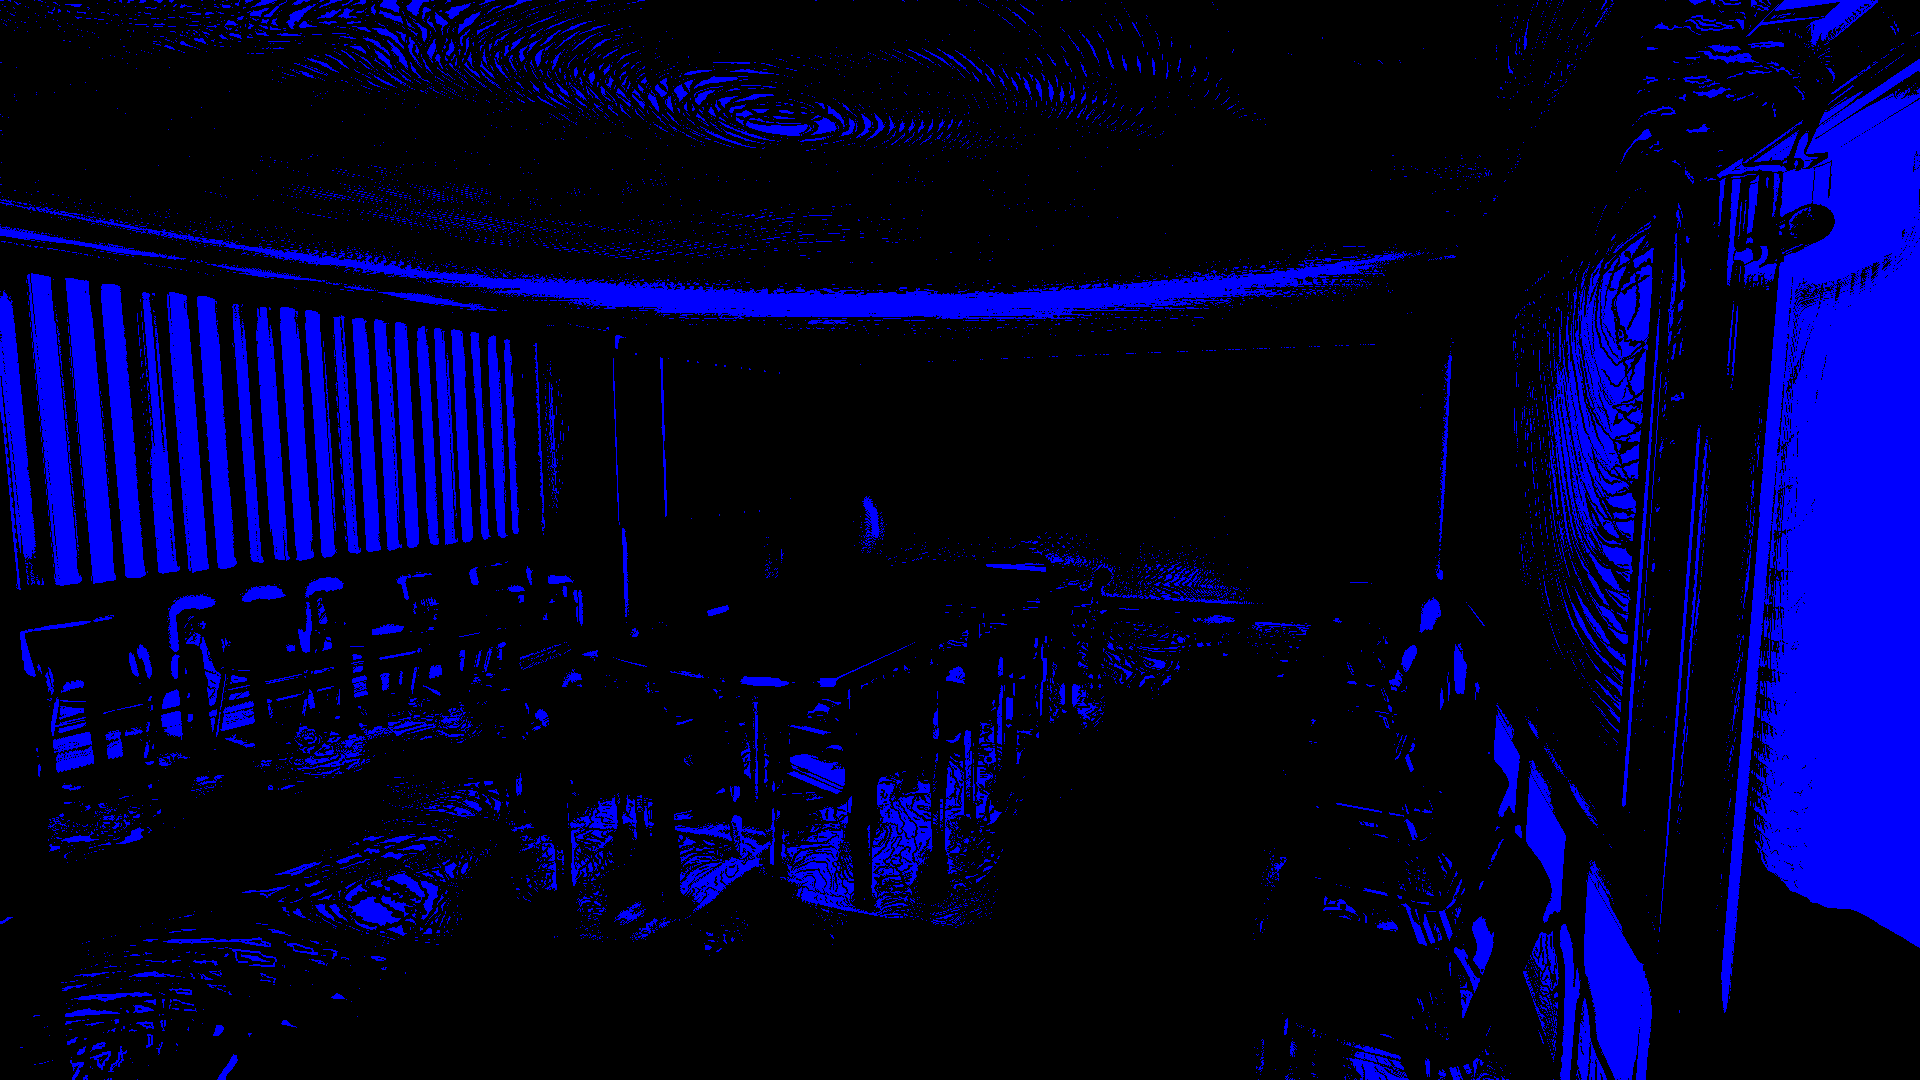
\includegraphics[width=\linewidth]{media/finals/conf_gi_128_diff.png}
		%\caption*{}
	\end{subfigure}%
	\par\smallskip
	\begin{subfigure}[b]{.49\linewidth}
		\centering
		\captionsetup{justification=centering}
		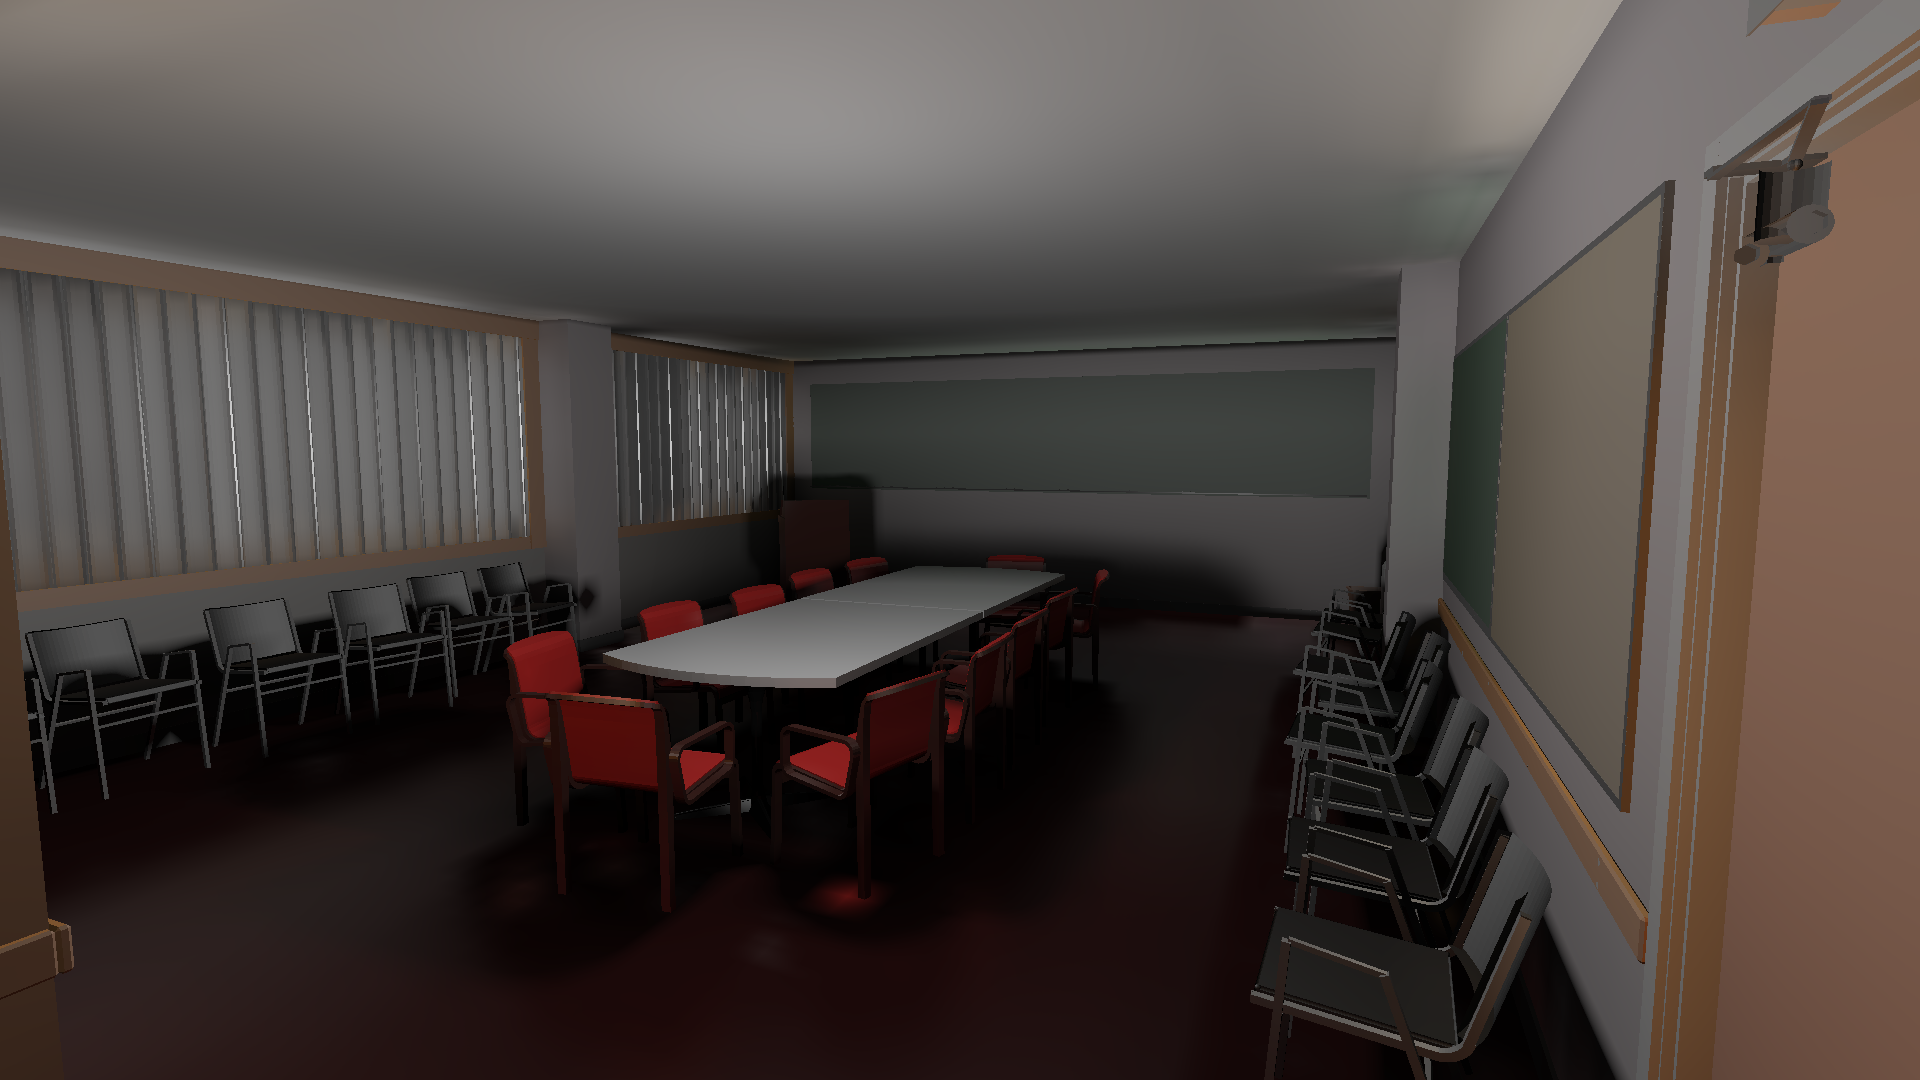
\includegraphics[width=\linewidth]{media/finals/conf_gi_64.png}
		%\caption*{$64^3$}
	\end{subfigure}%
	\hspace{0.01\textwidth}
	\begin{subfigure}[b]{.49\linewidth}
		\centering
		\captionsetup{justification=centering}
		%\caption*{Diferencia Perceptual}
		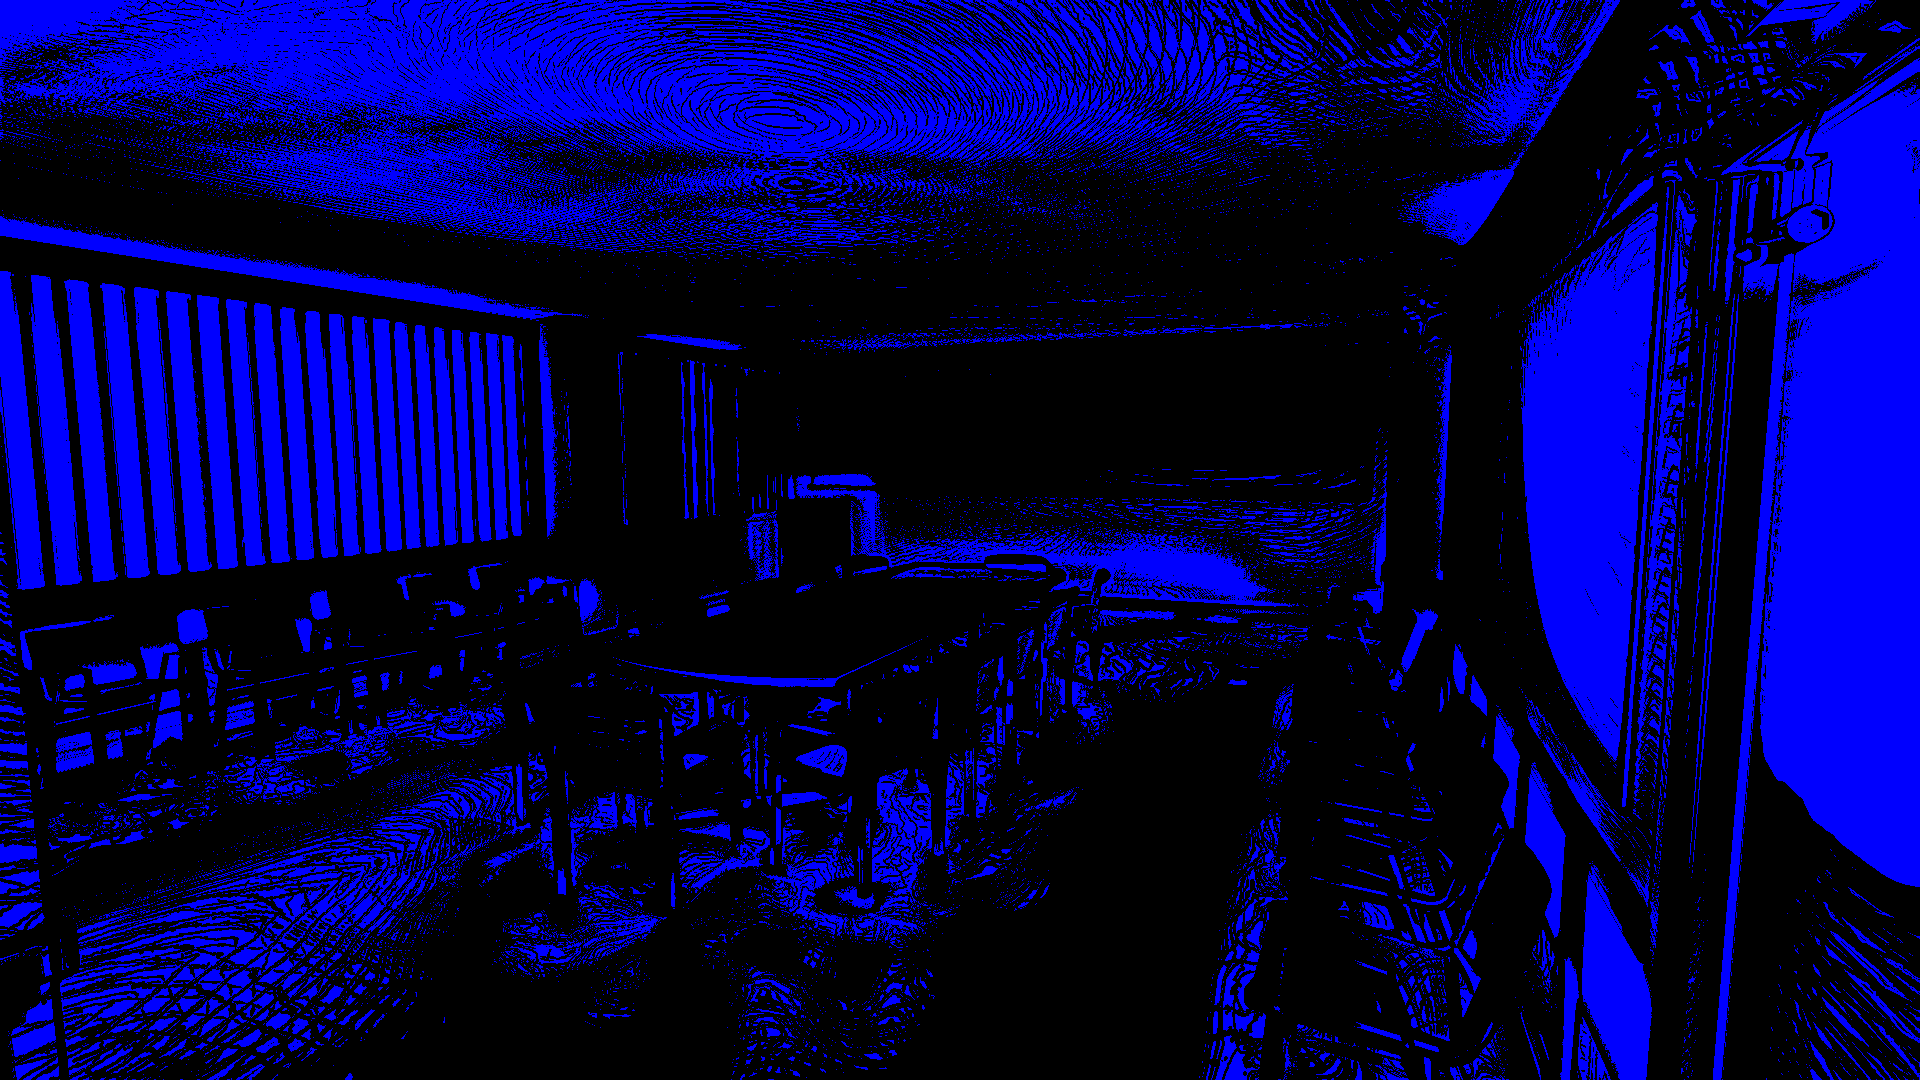
\includegraphics[width=\linewidth]{media/finals/conf_gi_64_diff.png}
		%\caption*{}
	\end{subfigure}%
	\caption{Diferencia visual con respecto a la imagen \ref{fig:conf_final} utilizando distintas resoluciones para la representación en vóxeles.}
	\label{fig:conf_gi_resdiff}
\end{figure}

\subsubsection{Factor de Longitud de Marcha del Cono}

El factor de longitud de marcha del cono afecta tanto el rendimiento como la calidad visual final. Valores mayores a $1.0$ no son recomendados ya que saltarían vóxeles constantemente durante el trazado. En esta sección comparamos contra el factor $0.5$ en la sección \ref{subsec:final} con valores de $1.0$ y $2.5$.


\begin{figure}[H]
	\centering
	\begin{subfigure}[b]{.49\linewidth}
		\centering
		\captionsetup{justification=centering}
		\caption*{Directa, Indirecta y Oclusión Ambiental}
		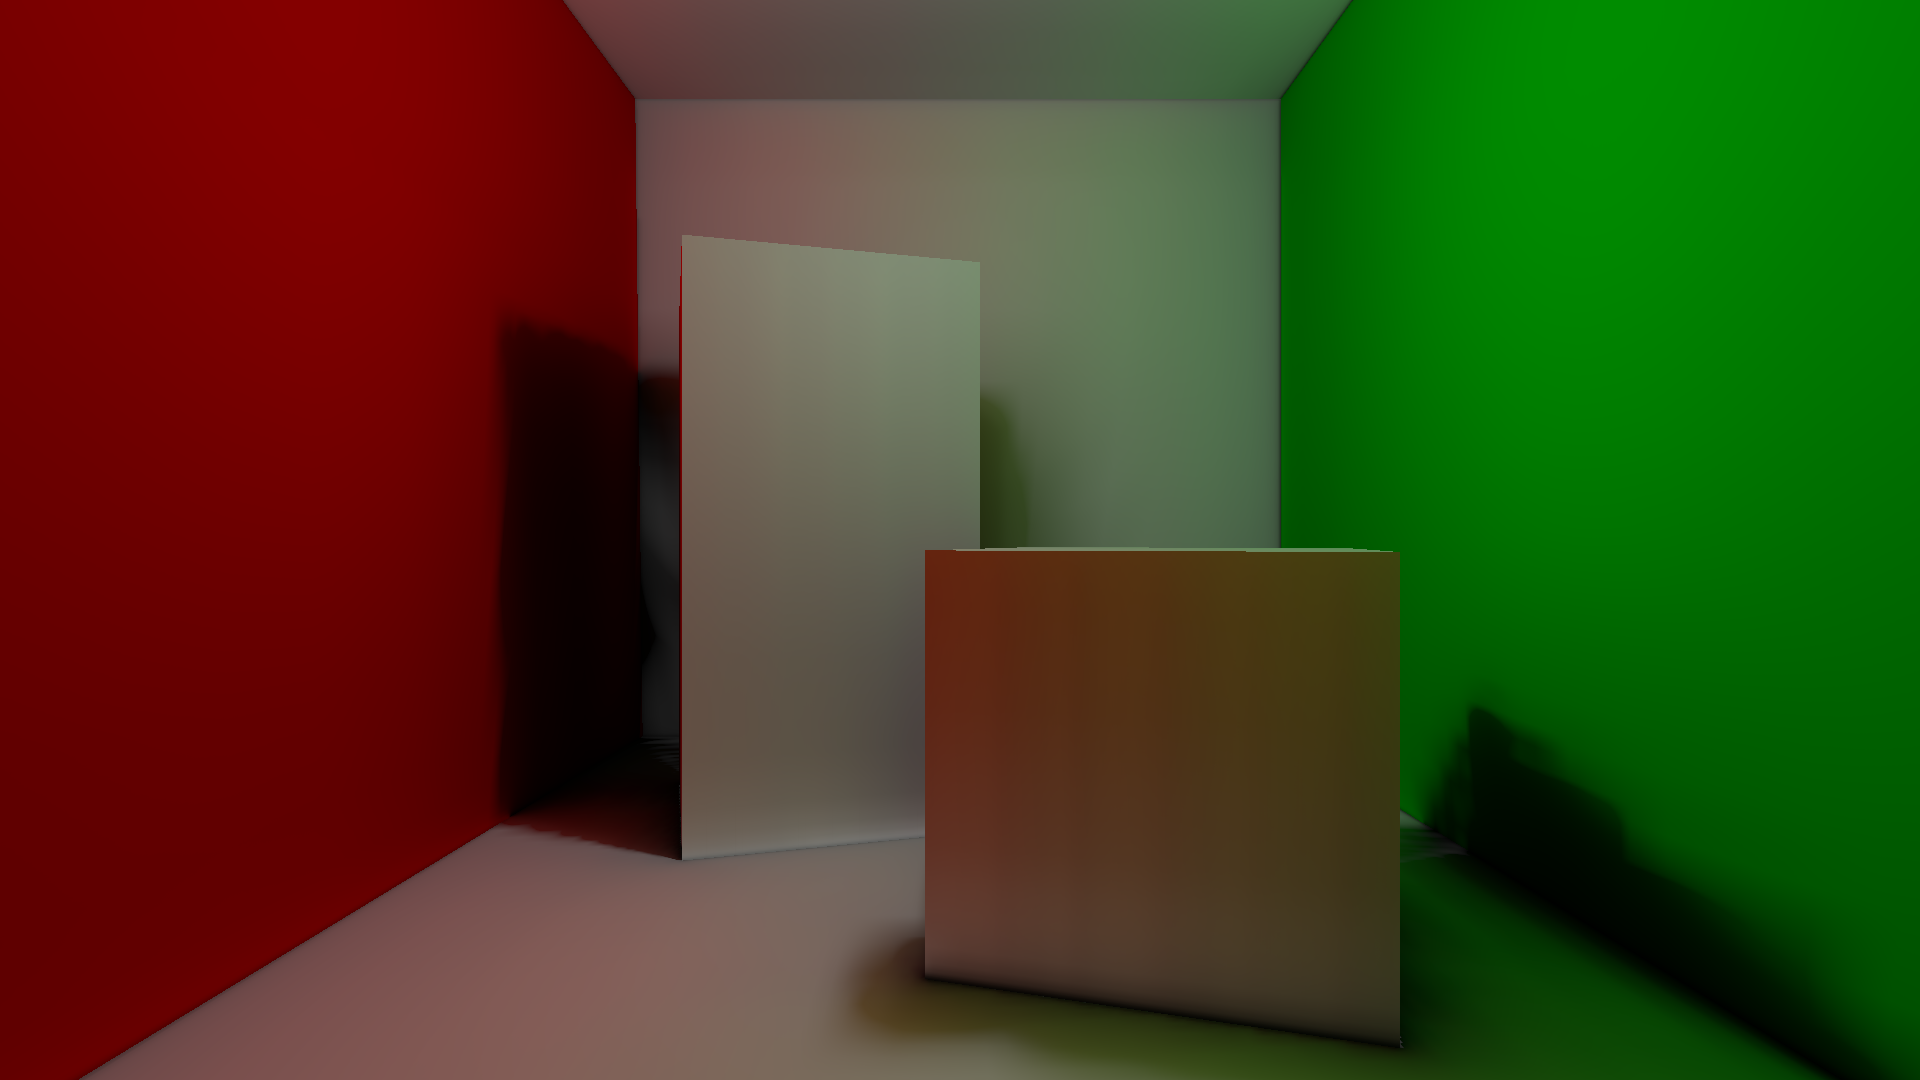
\includegraphics[width=\linewidth]{{media/finals/cornell_gi_s1.0}.png}
		\caption*{$1.0$}
	\end{subfigure}%
	\hspace{0.01\textwidth}
	\begin{subfigure}[b]{.49\linewidth}
		\centering
		\captionsetup{justification=centering}
		\caption*{Diferencia Perceptual\\}
		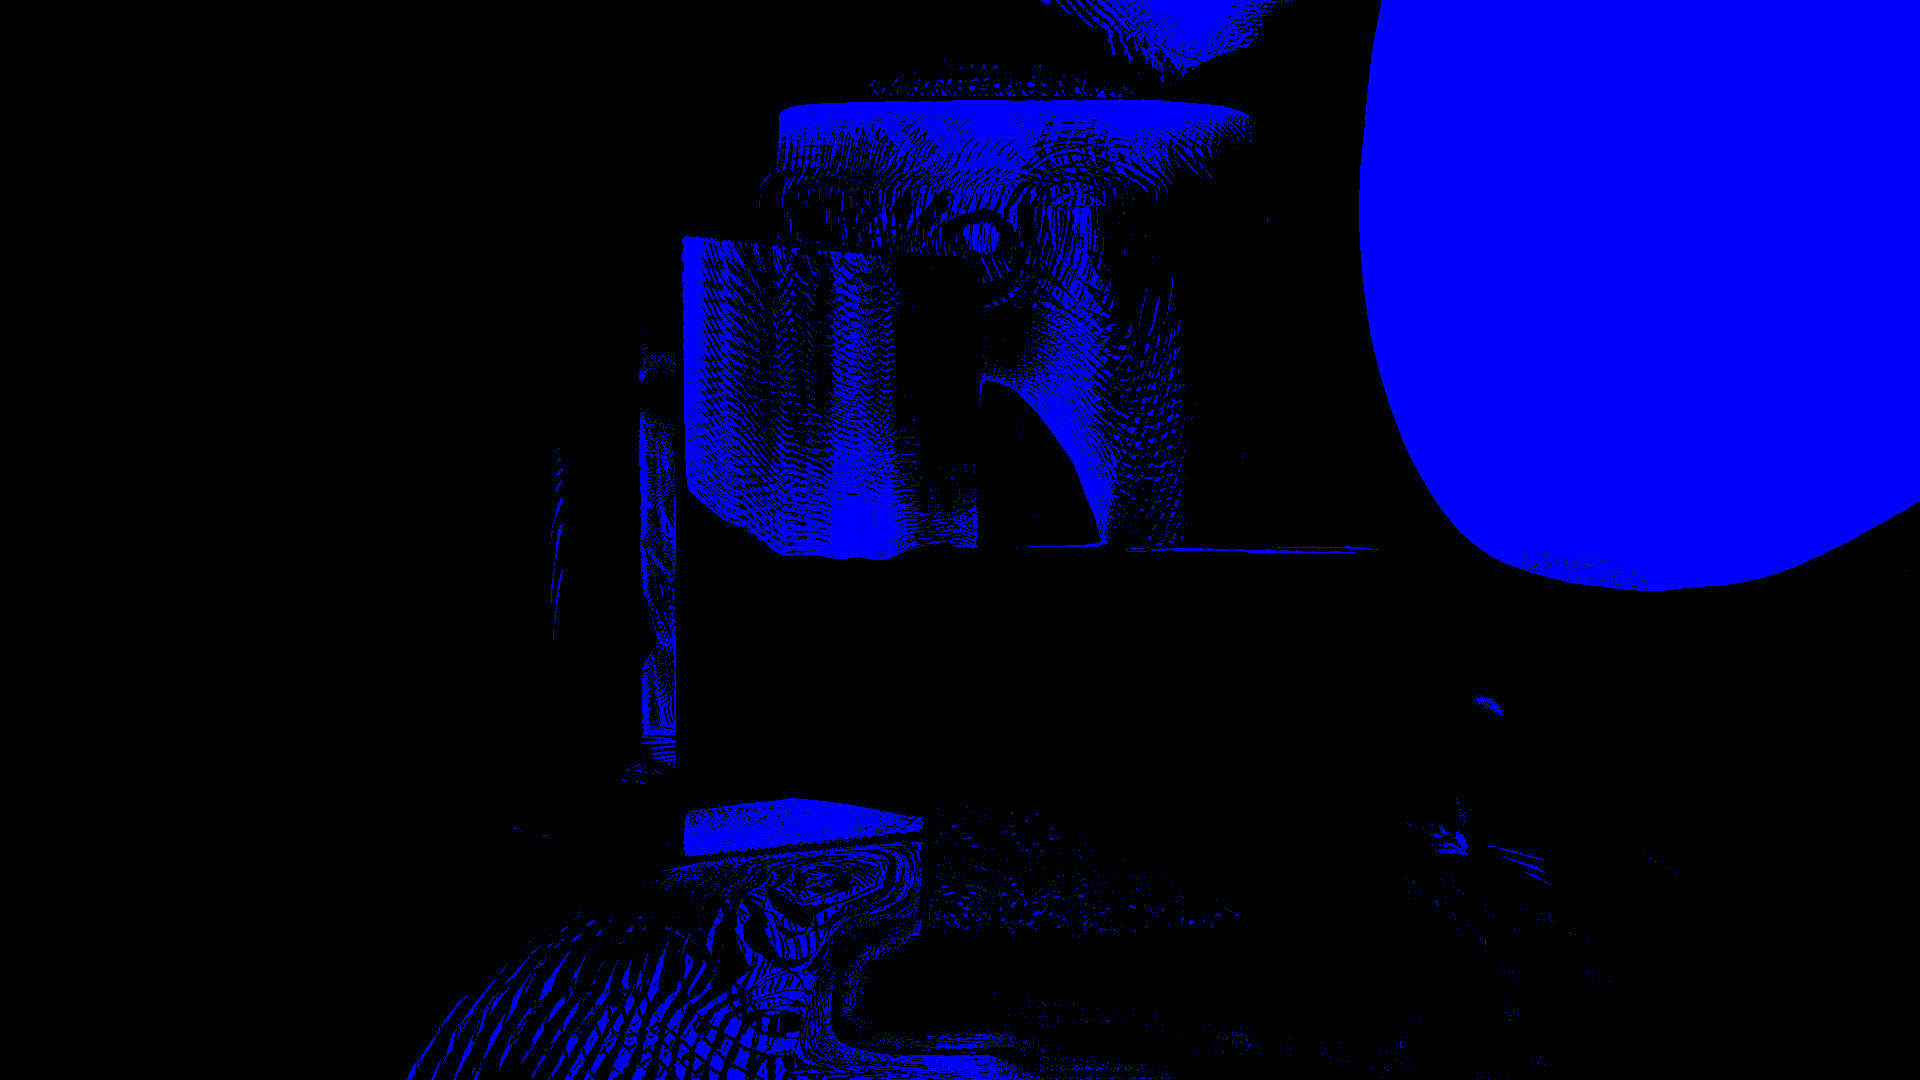
\includegraphics[width=\linewidth]{{media/finals/cornell_gi_s1.0_diff}.png}
		\caption*{}
	\end{subfigure}%
	\par\smallskip
	\begin{subfigure}[b]{.49\linewidth}
		\centering
		\captionsetup{justification=centering}
		\includegraphics[width=\linewidth]{{media/finals/cornell_gi_s2.5}.png}
		\caption*{$2.5$}
	\end{subfigure}%
	\hspace{0.01\textwidth}
	\begin{subfigure}[b]{.49\linewidth}
		\centering
		\captionsetup{justification=centering}
		%\caption*{Diferencia Perceptual}
		\includegraphics[width=\linewidth]{{media/finals/cornell_gi_s2.5_diff}.png}
		\caption*{}
	\end{subfigure}%
	\caption{Diferencia visual con respecto a la imagen \ref{fig:cornell_final} utilizando distintos factores de longitud.}
	\label{fig:cornell_gi_sdiff}
\end{figure}

\begin{figure}[H]
	\centering
	\begin{subfigure}[b]{.49\linewidth}
		\centering
		\captionsetup{justification=centering}
		%\caption*{Directa, Indirecta y Oclusión Ambiental}
		\includegraphics[width=\linewidth]{{media/finals/sibenik_gi_s1.0}.png}
		%\caption*{$1.0$}
	\end{subfigure}%
	\hspace{0.01\textwidth}
	\begin{subfigure}[b]{.49\linewidth}
		\centering
		\captionsetup{justification=centering}
		%\caption*{Diferencia Perceptual\\}
		\includegraphics[width=\linewidth]{{media/finals/sibenik_gi_s1.0_diff}.png}
		%\caption*{}
	\end{subfigure}%
	\par\smallskip
	\begin{subfigure}[b]{.49\linewidth}
		\centering
		\captionsetup{justification=centering}
		\includegraphics[width=\linewidth]{{media/finals/sibenik_gi_s2.5}.png}
		%\caption*{$2.5$}
	\end{subfigure}%
	\hspace{0.01\textwidth}
	\begin{subfigure}[b]{.49\linewidth}
		\centering
		\captionsetup{justification=centering}
		%\caption*{Diferencia Perceptual}
		\includegraphics[width=\linewidth]{{media/finals/sibenik_gi_s2.5_diff}.png}
		%\caption*{}
	\end{subfigure}%
	\caption{Diferencia visual con respecto a la imagen \ref{fig:sibenik_final} utilizando distintos factores de longitud.}
	\label{fig:sibenik_gi_sdiff}
\end{figure}

\begin{figure}[H]
	\centering
	\begin{subfigure}[b]{.49\linewidth}
		\centering
		\captionsetup{justification=centering}
		%\caption*{Directa, Indirecta y Oclusión Ambiental}
		\includegraphics[width=\linewidth]{{media/finals/conf_gi_s1.0}.png}
		%\caption*{$1.0$}
	\end{subfigure}%
	\hspace{0.01\textwidth}
	\begin{subfigure}[b]{.49\linewidth}
		\centering
		\captionsetup{justification=centering}
		%\caption*{Diferencia Perceptual\\}
		\includegraphics[width=\linewidth]{{media/finals/conf_gi_s1.0_diff}.png}
		%\caption*{}
	\end{subfigure}%
	\par\smallskip
	\begin{subfigure}[b]{.49\linewidth}
		\centering
		\captionsetup{justification=centering}
		\includegraphics[width=\linewidth]{{media/finals/conf_gi_s2.5}.png}
		%\caption*{$2.5$}
	\end{subfigure}%
	\hspace{0.01\textwidth}
	\begin{subfigure}[b]{.49\linewidth}
		\centering
		\captionsetup{justification=centering}
		%\caption*{Diferencia Perceptual}
		\includegraphics[width=\linewidth]{{media/finals/conf_gi_s2.5_diff}.png}
		%\caption*{}
	\end{subfigure}%
	\caption{Diferencia visual con respecto a la imagen \ref{fig:conf_final} utilizando distintos factores de longitud.}
	\label{fig:conf_gi_sdiff}
\end{figure}

\begin{figure}[H]
	\centering
	\begin{subfigure}[b]{.49\linewidth}
		\centering
		\captionsetup{justification=centering}
		%\caption*{Directa, Indirecta y Oclusión Ambiental}
		\includegraphics[width=\linewidth]{{media/finals/sponza_gi_s1.0}.png}
		%\caption*{$1.0$}
	\end{subfigure}%
	\hspace{0.01\textwidth}
	\begin{subfigure}[b]{.49\linewidth}
		\centering
		\captionsetup{justification=centering}
		%\caption*{Diferencia Perceptual\\}
		\includegraphics[width=\linewidth]{{media/finals/sponza_gi_s1.0_diff}.png}
		%\caption*{}
	\end{subfigure}%
	\par\smallskip
	\begin{subfigure}[b]{.49\linewidth}
		\centering
		\captionsetup{justification=centering}
		\includegraphics[width=\linewidth]{{media/finals/sponza_gi_s2.5}.png}
		%\caption*{$2.5$}
	\end{subfigure}%
	\hspace{0.01\textwidth}
	\begin{subfigure}[b]{.49\linewidth}
		\centering
		\captionsetup{justification=centering}
		%\caption*{Diferencia Perceptual}
		\includegraphics[width=\linewidth]{{media/finals/sponza_gi_s2.5_diff}.png}
		%\caption*{}
	\end{subfigure}%
	\caption{Diferencia visual con respecto a la imagen \ref{fig:sponza_final} utilizando distintos factores de longitud.}
	\label{fig:sponza_gi_sdiff}
\end{figure}

\subsection{Reflexión Especular y Factor de Longitud de Marcha}

El factor de longitud afecta especialmente la calidad de las reflexiones especulares finas. En el siguiente análisis se puede observar como empiezan a aparecer anomalías y vacíos en la reflexión especular a medida que se aumenta el factor de longitud.

\begin{figure}[H]
	\centering
	\includegraphics[width=.85\linewidth]{media/finals/test_s010.png}
	\caption{Demostración de reflexión especular con factor de longitud de marcha $0.1$ y volúmenes con resolución de $512^3$}
	\label{fig:spec_reflec010}
	\begin{subfigure}[b]{.49\linewidth}
		\centering
		\captionsetup{justification=centering}
		\caption*{$0.25$}
		%\caption*{Directa, Indirecta y Oclusión Ambiental}
		\includegraphics[width=\linewidth]{media/finals/test_s025.png}
	\end{subfigure}%
	\hspace{0.01\textwidth}
	\begin{subfigure}[b]{.49\linewidth}
		\centering
		\captionsetup{justification=centering}
		\caption*{}
		%\caption*{Diferencia Perceptual\\}
		\includegraphics[width=\linewidth]{media/finals/test_s025_diff.png}
	\end{subfigure}%
	\par\smallskip
	\begin{subfigure}[b]{.49\linewidth}
		\centering
		\captionsetup{justification=centering}
		\caption*{$0.5$}
		\includegraphics[width=\linewidth]{media/finals/test_s050.png}
	\end{subfigure}%
	\hspace{0.01\textwidth}
	\begin{subfigure}[b]{.49\linewidth}
		\centering
		\captionsetup{justification=centering}
		\caption*{}
		%\caption*{Diferencia Perceptual}
		\includegraphics[width=\linewidth]{media/finals/test_s050_diff.png}
	\end{subfigure}%	
\end{figure}
\begin{figure}[H]
	\centering
	\begin{subfigure}[b]{.49\linewidth}
		\centering
		\captionsetup{justification=centering}
		\caption*{$1.0$}
		\includegraphics[width=\linewidth]{media/finals/test_s100.png}
	\end{subfigure}%
	\hspace{0.01\textwidth}
	\begin{subfigure}[b]{.49\linewidth}
		\centering
		\captionsetup{justification=centering}
		\caption*{}
		%\caption*{Diferencia Perceptual}
		\includegraphics[width=\linewidth]{media/finals/test_s100_diff.png}
	\end{subfigure}%
	\par\smallskip
	\begin{subfigure}[b]{.49\linewidth}
		\centering
		\captionsetup{justification=centering}
		\caption*{$2.5$}
		\includegraphics[width=\linewidth]{media/finals/test_s250.png}
	\end{subfigure}%
	\hspace{0.01\textwidth}
	\begin{subfigure}[b]{.49\linewidth}
		\centering
		\captionsetup{justification=centering}
		\caption*{}
		%\caption*{Diferencia Perceptual}
		\includegraphics[width=\linewidth]{media/finals/test_s250_diff.png}
	\end{subfigure}%
	\caption{Diferencia con respecto a la imagen \ref{fig:spec_reflec010} considerando distintos factores de longitud. Se puede observar como este factor afecta de gran manera la calidad de las reflexiones sobre distintas superficies especulares de esta escena.}
	\label{fig:spec_reflex_comp1}
\end{figure}

\subsection{Apertura del Cono para Trazado de Sombras Suaves}

Una de las características del trazado de conos es que mientras mayor es la apertura del cono más rápido es el trazado como ya fue estudiado en la figura \ref{fig:shadowcone_aperture}. Esto puede ser una ventaja para el trazado de sombras suaves ya que a medida que se abre el cono de sombreado más suaves son las sombras resultantes como veremos en las siguientes imágenes:

\begin{figure}[H]
	\centering
	\begin{subfigure}[b]{.49\linewidth}
		\centering
		\captionsetup{justification=centering}
		\caption*{Ángulo de apertura: 1 grado}
		\includegraphics[width=\linewidth]{media/finals/shadow_1.png}
	\end{subfigure}%
	\hspace{0.01\textwidth}
	\begin{subfigure}[b]{.49\linewidth}
		\centering
		\captionsetup{justification=centering}
		\caption*{5 grados}
		\includegraphics[width=\linewidth]{media/finals/shadow_5.png}
	\end{subfigure}%
	%\caption{Sombras suaves generadas bajo distintas aperturas del cono de sombreado.}
	%\label{fig:spec_reflex_comp1}
\end{figure}
\begin{figure}[H]
	\centering
	\begin{subfigure}[b]{.49\linewidth}
		\centering
		\captionsetup{justification=centering}
		\caption*{15 grados}
		\includegraphics[width=\linewidth]{media/finals/shadow_15.png}
	\end{subfigure}%
	\hspace{0.01\textwidth}
	\begin{subfigure}[b]{.49\linewidth}
		\centering
		\captionsetup{justification=centering}
		\caption*{25 grados}
		\includegraphics[width=\linewidth]{media/finals/shadow_25.png}
	\end{subfigure}%
	\caption{Sombras suaves generadas bajo distintas aperturas del cono de sombreado.}
	\label{fig:soft_aperture}
\end{figure}

%\subsubsection{Mapeo del Volumen de Visibilidad}


\subsection{Materiales Emisivos}

Nuestra implementación permite la aproximación de materiales emisivos con la adición de otro volumen durante el proceso de voxelización. Estos materiales pueden ser utilizados para simular luces de área. En esta sección se puede observar estos materiales en acción.

\begin{figure}[H]
	\centering
	\includegraphics[width=\linewidth]{media/finals/area_teapot.png}
	\caption{En esta escena no hay fuentes de luz, el modelo de Utah Teapot tiene un material emisivo blanco que ilumina el resto de los objetos cercanos. La oclusión ambiental esta desactivada para esta imagen las sombras debajo de los objetos son generadas de forma natural por el trazado de conos contra vóxeles.}
	\label{fig:areapot}
\end{figure}

\begin{figure}[H]
	\centering
	\includegraphics[width=\linewidth]{media/finals/area_sponza.png}
	\caption{Escena Sponza iluminada por varios materiales emisivos de distintos colores.}
	\label{fig:areasponza}
\end{figure}

\begin{figure}[H]
	\centering
	\includegraphics[width=\linewidth]{media/finals/area_shadows.png}
	\caption{Sombras suaves generadas por materiales emisivos. En esta imagen es notable la dirección de las sombras según la fuente de iluminación.}
	\label{fig:areashadows}
\end{figure}


\begin{figure}[H]
	\centering
	\includegraphics[width=\linewidth]{media/finals/fine_emissive.png}
	\caption{Detalles finos en materiales con emisión utilizando texturizado.}
	\label{fig:fine_emissive}
\end{figure}
